\documentclass[
	12pt, 
	a4paper, 
	parskip=false,
	listof=totoc,
	bibliography=totoc,
	index=totoc,
	toc=chapterentrywithdots,
	numbers=noenddot,
]{scrreprt}  % Changed from scrbook to scrreprt

% Essential packages and settings
\usepackage{bookmark}

\usepackage[american]{babel}
\usepackage{url}
\usepackage[autostyle=true,german=quotes]{csquotes}
\usepackage[T1]{fontenc}
\usepackage{pdfpages}
\usepackage{textcomp}
\usepackage{amsmath}
\usepackage{fontspec}
\usepackage{unicode-math}
\usepackage{siunitx}

% Consolidated bibliography configuration with Mendeley integration
\usepackage[backend=biber,style=apa,citestyle=apa,autolang=other]{biblatex}
\addbibresource{sources/mendeley.bib}

% Compatibility commands for PGF figures
\providecommand{\mathdefault}{\mathnormal}
\providecommand{\mathdefault}[1]{#1}

\usepackage{pgf}
\usepackage{layouts}
\usepackage{caption}
\usepackage{lmodern}

% PDF metadata configuration
\usepackage{hyperref}
\hypersetup{
  pdfauthor={Lukas Michael},
  pdftitle={Machine Learning for Systematic New Issue Premium Identification and Portfolio Optimization in European Corporate Bond Markets},
  pdfsubject={Bachelor Thesis},
  pdfkeywords={Machine Learning; XGBoost; New Issue Premium; European Corporate Bonds; Investment-Grade; Portfolio Optimization; Fixed Income; Systematic Investing; Feature Engineering; Classification Algorithm; Short-term Excess Returns},
  pdfproducer={LaTeX},
}

% Include additional settings files
% graphics
\usepackage{graphicx}
\graphicspath{ {images/} }
\DeclareGraphicsExtensions{.pdf,.png,.jpg,.jpeg,.gif}

% APA 7 compliant captions - main configuration handled in tables.tex
% This ensures consistency across figures and tables
\usepackage{caption}
\usepackage{subcaption}

% Subcaption formatting for APA compliance
\captionsetup[sub]{
  font={normalsize},
  labelfont={bf},
  labelsep=period,
  justification=justified
}
% Table layout
\setlength{\tabcolsep}{0.5em} % for the horizontal padding
\renewcommand{\arraystretch}{1.2} % for the vertical padding

% Table captions
\usepackage{caption} 
\captionsetup[table]{belowskip=12pt,aboveskip=4pt}
\usepackage{diagbox}

% Rotate tables
\usepackage{rotating}
\usepackage{varwidth}

% Footnotes with tables
\usepackage{footnote}
\makesavenoteenv{figure}

% Line breaks in table cells
\newcommand{\specialcell}[2][c]{%
  \begin{tabular}[#1]{@{}c@{}}#2\end{tabular}
}

% rotate content of table cell
\def\rot{\rotatebox} % usage: \rot{angle}{content}

% booktabs table
\usepackage{booktabs}

\input{settings/colors.tex}
% geometry - Updated margins for APA 7 (1-inch margins)
\usepackage{geometry}
\geometry{left=25.4mm, right=25.4mm, top=25.4mm, bottom=25.4mm}

\usepackage[automark]{scrlayer-scrpage}
\pagestyle{plain}

% footnote gap
\addtolength{\skip\footins}{1ex}
\addtolength{\footnotesep}{0.5ex}

% prevent footnote page break
\interfootnotelinepenalty=10000

% line spacing
\usepackage[onehalfspacing]{setspace}

% text does not have to go to the end of a page
\raggedbottom

% APA 7 compliant paragraph formatting
\setlength{\parindent}{0.5in}  % APA paragraph indent
\setlength{\parskip}{0pt}      % No extra space between paragraphs

% APA 7 compliant chapter formatting - simplified and standardized
\RedeclareSectionCommand[
  beforeskip=0pt,
  afterskip=12pt,
  font=\normalfont\bfseries\fontsize{12}{18}\selectfont
]{chapter}

% APA 7 compliant section heading hierarchy
\RedeclareSectionCommands[
  beforeskip=12pt,
  afterskip=6pt,
  font=\normalfont\bfseries
]{section,subsection,subsubsection}

\usepackage{mwe}

% Remove custom chapter format for APA compliance - use standard formatting
\setkomafont{disposition}{\normalcolor\bfseries}
\setkomafont{paragraph}{\normalsize}

% layout of the paragraphs
% paragraphs look like the subsubsections
\RedeclareSectionCommands[
    beforeskip=-3.25ex plus -1ex minus -0.2ex,
    afterskip=1sp, % smallest possible positive value
]{paragraph,subparagraph}

% Bold caption labels - moved to dedicated caption settings
\setkomafont{captionlabel}{\normalsize\bfseries}
\usepackage{listings}
\usepackage[many]{tcolorbox}

% name of listings in the toc
\renewcommand\lstlistlistingname{Listingverzeichnis}

% general settings for listing
\lstset{
    xleftmargin=1.1cm,
    belowskip=2em,
    basicstyle=\fontsize{10}{15}\ttfamily,
    basewidth  = {.5em,0.4em},
    captionpos=t,
    lineskip={2pt},
    backgroundcolor=\color{white},
    framextopmargin=6pt,
    framexrightmargin=0pt,
    framexleftmargin=0.9em,    
    framexbottommargin=6pt, 
    frame=l,
%    frame=single,        
%    frame=tb, framerule=0pt,    
    framesep=6.5mm,
    fillcolor=\color{white},
    rulecolor=\color{middlegray},
    numbers=left,
    numberstyle=\normalfont\color{middlegray},
%    numberstyle=\footnotesize,    
    numbersep=10pt,
    abovecaptionskip=10pt, %space above the caption
    belowcaptionskip=10pt, %space below the caption
    extendedchars=true,
    showstringspaces=false,
    showspaces=false,
    stepnumber=1, % the step between two line-numbers. If it is 1 each line will be numbered
    tabsize=2,
    breaklines=true,
    showtabs=false,
    upquote=true,
    % German umlauts
    literate=%
    {Ö}{{\"O}}1
    {Ä}{{\"A}}1
    {Ü}{{\"U}}1
    {ß}{{\ss}}1
    {ü}{{\"u}}1
    {ä}{{\"a}}1
    {ö}{{\"o}}1
}

% define language
\lstdefinelanguage{JavaScript}{
    keywords={typeof, new, true, false, catch, then, function, return, null, catch, switch, var, if, in, while, do, else, case, break, default},
    keywordstyle=\color{editorGreen}\bfseries,
    ndkeywords={class, export, boolean, throw, implements, import, this, const},
    ndkeywordstyle=\color{vscodeblue}\bfseries,
    identifierstyle=\color{black},
    sensitive=false,
    comment=[l]{//},
    morecomment=[s]{/*}{*/},
    commentstyle=\color{editorGreen}\ttfamily,
    stringstyle=\color{darkred}\ttfamily,
    morestring=[b]',
    morestring=[b]"
}

\lstdefinelanguage{SQL}{
    keywords={select, where, from},
    keywordstyle=\color{editorGreen}\bfseries,
    ndkeywords={},
    ndkeywordstyle=\color{vscodeblue}\bfseries,
    identifierstyle=\color{black},
    sensitive=false,
    comment=[l]{--},
    morecomment=[s]{/*}{*/},
    commentstyle=\color{editorGreen}\ttfamily,
    stringstyle=\color{darkred}\ttfamily,
    morestring=[b]',
    morestring=[b]"
}


\lstdefinelanguage{HTML5}{
  language=html,
  sensitive=true,	
  alsoletter={<>=-},	
  morecomment=[s]{<!-}{-->},
  tag=[s],
  otherkeywords={
  % General
  >,
  % Standard tags
	<!DOCTYPE,
  </html, <html, <head, <title, </title, <style, </style, <link, </head, <meta, />,
	% body
	</body, <body,
	% Divs
	</div, <div, </div>, 
	% Paragraphs
	</p, <p, </p>,
	% scripts
	</script, <script,
  % More tags...
  <canvas, /canvas>, <svg, <rect, <animateTransform, </rect>, </svg>, <video, <source, <iframe, </iframe>, </video>, <image, </image>, <header, </header, <article, </article
  },
  ndkeywords={
  % General
  =,
  % HTML attributes
  charset=, src=, id=, width=, height=, style=, type=, rel=, href=,
  % SVG attributes
  fill=, attributeName=, begin=, dur=, from=, to=, poster=, controls=, x=, y=, repeatCount=, xlink:href=,
  % properties
  margin:, padding:, background-image:, border:, top:, left:, position:, width:, height:, margin-top:, margin-bottom:, font-size:, line-height:,
	% CSS3 properties
  transform:, -moz-transform:, -webkit-transform:,
  animation:, -webkit-animation:,
  transition:,  transition-duration:, transition-property:, transition-timing-function:,
  }
}

\lstdefinestyle{html} {%
  % Code design
  keywordstyle=\color{lightblack}\bfseries,
  ndkeywordstyle=\color{lightblack}\bfseries,
  identifierstyle=\color{lightblack},
  commentstyle=\color{green}\ttfamily,
  stringstyle=\color{darkred}\ttfamily,
  % Code
  language=HTML5,
%  alsolanguage=JavaScript,
  alsodigit={.:;},	
  tabsize=2,
  showtabs=false,
  showspaces=false,
  showstringspaces=false,
  extendedchars=true,
  breaklines=true,
  % German umlauts
  literate=%
  {Ö}{{\"O}}1
  {Ä}{{\"A}}1
  {Ü}{{\"U}}1
  {ß}{{\ss}}1
  {ü}{{\"u}}1
  {ä}{{\"a}}1
  {ö}{{\"o}}1
}

\lstdefinelanguage{CSS} 
{morekeywords={color,background,margin,padding,margin,padding,font,weight,display,position,top,left,right,bottom,list,style,border,size,white,space,min,width, 	transition}, 
	sensitive=false, 
	morecomment=[l]{//}, 
	morecomment=[s]{/*}{*/}, 
	morestring=[b]", 
}

\lstdefinestyle{css} {%
  language=CSS,
  keywordstyle=\color{lightblack},
}

\lstdefinestyle{js} {
  language=JavaScript
}

\lstdefinestyle{sql} {
  language=SQL,
  keywordstyle=\color{azure}  
}

%Usage
%\begin{minipage}{\linewidth}
%\begin{lstlisting}[style=js, caption={Flux Action Creator}, label=lst:actionCreator] 
%create: function(text) {
  %AppDispatcher.dispatch({
    %type: Constants.TODO_CREATE,
    %payload: 'sample'
  %});
%},
%\end{lstlisting}
%\end{minipage}
% for the links in toc

\hypersetup{
    colorlinks,
    citecolor=black,
    filecolor=black,
    linkcolor=black,
    urlcolor=black,
    pdfstartview= % fit zoom size to the viewer
}
% This "\code{my code}" can be used to highlight small code snippets in the text like names of variables or methods.
\newcommand{\code}[1]{\textcolor{black}{\texttt{#1}}}

% The "\todo{this still has to be done}" is a command that highlights todos in the text.
\newcommand{\todo}[1]{\textcolor{vscodered}{TODO: \texttt{#1}}}

\begin{document}

% -------------------
% |    Titlepage    |
% -------------------
\begin{titlepage}
    \thispagestyle{empty}
    
    % Logo positioning - top right corner
    \hfill
\includegraphics[height=2cm]{images/logo.pdf}
    
    \vspace{2cm}
    
    % Main content centered
    \begin{center}
        
        % Bachelor Thesis heading
        {\Huge \textbf{Bachelor Thesis}}\\
        \vspace{1.5cm}
        
        % Title
        {\LARGE \textbf{Machine Learning for Systematic New Issue Premium Identification and Portfolio Optimization in European Investment Grade Corporate Bond Markets}}\\
        \vspace{2cm}
        
        % Chair information
        {\large Chair of Empirical Capital Market Research}\\
        \vspace{0.5cm}
        
        {\large Prof. Dr. Johanning Lutz}\\
        \vspace{0.2cm}
        
        {\large Dr. Philip Schnorpfeil}\\
        \vspace{2cm}
        
        % Date and location
        {\large Vallendar, 27.05.2025}\\
        \vspace{1.5cm}
        
        % Student information
        {\large \textbf{Lukas, Michael}}\\
        \vspace{0.5cm}
        
        {\large 20006749}\\
        \vspace{0.2cm}
        
        {\large 06.07.2002, Lörrach}\\
        \vspace{0.2cm}
        
        {\large Elbinger Weg, 2a, 40474 Düsseldorf}\\
        
    \end{center}
    
\end{titlepage}

% ------------------
% |    Abstract    |
% ------------------
\pagenumbering{roman}
\setcounter{page}{1}
\pdfbookmark[section]{Kurzfassung}{abstract}
\chapter*{Abstract}
\thispagestyle{empty} %hide page numbers

Despite the documented existence of new issue premiums in credit markets, no systematic machine learning approach has been developed to identify these opportunities in European investment-grade corporate bond markets, where traditional selection methods rely heavily on subjective judgment and experience-based analysis. This research addresses this gap by developing the first comprehensive framework that transforms bond characteristics and macroeconomic conditions into actionable investment signals using extreme gradient boosting (XGBoost).

Through an analysis of European investment grade bond issuances from 2000 to 2025, the study demonstrates that there are systematic patterns in the pricing of new issues that can be exploited quantitatively, even within relatively efficient markets. The machine learning framework achieves high precision in identifying outperforming bonds while generating meaningful risk-adjusted returns with consistent performance under varying market conditions. Key predictive features include first-time issuer status, credit risk indicators, and macroeconomic factors such as market direction and inflation dynamics.

These findings establish that quantitative methods can meaningfully improve traditional investment decision-making in European corporate bond markets. The framework provides portfolio managers with a systematic tool for alpha generation while maintaining appropriate risk controls, potentially transforming how fixed income professionals approach the evaluation and selection of new issues in institutional investment environments.

% ---------------------------
% |    Table of contents    |
% ---------------------------
\pdfbookmark[section]{\contentsname}{toc}
\tableofcontents

% -----------------
% |    Indexes    |
% -----------------
\listoffigures
\listoftables

% ------------------
% |    Chapters    |
% ------------------
\pagenumbering{arabic}
\setcounter{page}{1}
\chapter{Introduction}
\label{introduction}
\setcounter{page}{1}

The new issue premium (NIP) represents a well-documented phenomenon in fixed-income markets where newly issued bonds are priced at a discount to comparable outstanding securities, creating potential excess returns for investors who participate in primary market offerings. While extensive research has established the existence of this premium across various credit segments, with particular emphasis on high-yield securities \parencite{Geerts2022PredictingYield}, a significant gap remains in understanding how predictive modeling can systematically identify new issue premium opportunities within the European investment-grade corporate bond market.

Existing literature demonstrates that the magnitude of new issue premiums varies considerably across credit quality segments, with high-yield bonds typically exhibiting the most substantial premiums while investment-grade securities show more modest and inconsistent patterns \parencite{Traczyk2024NewFactor}. This characteristic poses particular challenges for investment-grade focused strategies, where the lower base rate of outperforming issuances necessitates more sophisticated selection methodologies to generate meaningful excess returns. Despite the documented presence of new issue premiums in investment-grade markets, no systematic machine learning approach has been developed specifically for European investment-grade corporate bonds that transforms issuer and market characteristics into actionable investment signals.

Current industry practice in fixed-income investment teams centers on participating in new issuances as a primary strategy for generating portfolio returns through new issue premium capture. The conventional approach typically employs relative valuation frameworks that position potential investments within peer group comparisons, often visualized through scatter plot analyses plotting maturity against credit spreads to identify bonds trading wider than comparable securities\footnote{This observation is based on personal experience during an internship with a fixed-income investment team in 2024.}. While this methodology incorporates substantial manual research, institutional experience, and qualitative assessments, it frequently limits quantitative analysis to a narrow set of immediately observable characteristics at the time of issuance. The decision-making process predominantly relies on subjective judgments and experience-based evaluations, potentially overlooking systematic patterns present in comprehensive historical datasets. Given the extensive availability of past bond issuance data and the demonstrated effectiveness of machine learning algorithms in binary classification tasks, significant opportunities exist to enhance traditional selection methodologies through automated, systematic approaches that can serve as initial screening mechanisms to complement existing analytical frameworks.

This research addresses the fundamental question of whether machine learning algorithms can reliably predict new issue premium opportunities in European investment-grade corporate bonds and whether such predictions can form the basis for enhanced investment decision-making processes. The investigation employs a comprehensive dataset of 7,320 European investment-grade corporate bond issuances extracted from Refinitiv's fixed-income database, spanning the period from 2000 to 2025. Through systematic feature engineering incorporating both microeconomic bond characteristics and macroeconomic market conditions, a predictive framework using Extreme Gradient Boosting (XGBoost) is developed that classifies bonds according to their likelihood of short-term outperformance.

This research contributes to the fixed-income literature in three principal ways. First, it demonstrates the viability of machine learning approaches for systematic new issue premium identification in European investment-grade markets, extending existing methodologies beyond traditional high-yield applications to more conservative credit segments. Second, it identifies and validates specific microeconomic and macroeconomic features that exhibit predictive power for short-term bond performance, providing practical insights for fixed-income portfolio management. Third, it presents a systematic framework that translates machine learning predictions into actionable investment signals, offering portfolio managers enhanced tools for alpha generation while maintaining appropriate risk controls in institutional investment environments.
\chapter{Theory}
\label{ch:theory}

\section{Bond Market Fundamentals}

\subsection{Primary and Secondary Market}

Corporate bonds serve as a crucial funding mechanism for medium- and large-sized enterprises. These financial instruments allow companies to leverage bond sales for expansion initiatives and diversify their financing sources. The bond market operates in two separate segments: the primary market, where new bonds are initially created and sold to investors, and the secondary market, where previously issued bonds are traded among market participants. Unlike equity trading, which predominantly occurs on exchanges that bring together multiple buyers and sellers, corporate bond trading has traditionally relied on market makers. These market makers, typically banks or broker-dealers, simultaneously provide bid and ask prices for the same bonds. When bondholders initiate a sell transaction, market makers offer a "bid" price; conversely, when investors seek to acquire bonds, market makers present an "ask" price. The differential between these prices, known as the "bid-ask spread," represents the potential profit for market makers and compensates them for the risk associated with holding bonds in their inventory.

\subsection{New Issuance Premium}

Based on the new premium issue framework, the specific market mechanisms underlying this phenomenon operate through the syndicated issuance process, as explained in \parencite{Traczyk2024NewFactor}. This premium typically occurs in standard bearer bullet structures distributed through a syndicated format. In this process, the issuers engage a syndicate of banks to collect orders from potential investors within an order book. These issuances generally involve substantial volumes to establish sufficiently liquid secondary markets. To ensure adequate liquidity, syndicate banks aim for oversubscription in the order book by offering attractive pricing, specifically a premium over comparable bonds in the secondary market. 

A positive NIP indicates a favorable yield spread over similar bonds, resulting in a lower initial price for the newly issued bond, which subsequently yields greater returns as its yield converges with peer group bonds shortly after issuance. Although this premium is typically positive, its magnitude reflects the dynamics of price discovery during issuance, particularly the level of investor demand, which may occasionally result in negative premiums. Strong demand for a bond can enable issuers to secure funding at lower costs by allocating bonds at higher prices, thereby reducing effective yields and coupon rates.

From this framework, it becomes clear why exploiting the new issuance premium is attractive to investors. Many fixed-income fund managers regularly participate in new issuances to generate additional relatively predictable returns for their portfolios. According to \textcite[chap. 35]{Fabozzi2021TheEdition}, investment teams commonly employ a relative value credit approach to determine whether a bond carries a NIP. This analytical method compares the new bond's spread (such as z-spread, OAS, yield, etc.) against a basket of similarly rated bonds from the same sector with comparable maturity and seniority. As \textcite{Fabozzi2021TheEdition} further observes, the relative value based on the market vs. the relative value based on the model constitutes an important consideration in this analysis. Fund managers typically participate when new issues trade wider than comparable bonds; otherwise, they abstain. However, this approach requires considerable experience to make accurate predictions. Human error, particularly the failure to account for relevant factors that might indicate the absence of an NIP, can occur and potentially undermine fund performance.

\section{Machine Learning Fundamentals}

To better understand this paper's strategy, it is necessary to briefly examine the nature of machine learning, its operational mechanisms, and highlight XGBoost, the model employed in this research.

\textcite{Johari2018MachineExamples} defines machine learning as "a concept that allows the machine to learn from examples and experience, and that too without being explicitly programmed". She explains that machine learning inverts traditional programming approaches rather than explicitly writing code, data is provided to generic algorithms that construct logic based on the supplied information. Machine learning algorithms represent an evolution of conventional algorithms that enhance program intelligence by enabling data-based autonomous learning. The process typically divides into two primary phases: the Training Phase and the Testing Phase. During training, the algorithm processes labeled data samples to identify patterns and relationships. The testing phase subsequently evaluates the model's performance using previously unseen data. Unlike training data, testing data are only used after the model has been fully trained and refined. This data assesses the model's ability to generalize to novel scenarios and provides an unbiased evaluation of its accuracy, precision, and overall reliability.

XGBoost represents a highly effective machine learning methodology that has received significant attention for its exceptional performance in addressing classification and regression problems, as noted by \textcite{Harrison2023EffectiveModels}. This technique leverages an ensemble of decision trees to develop robust predictive models through iterative error minimization. In this context, gradient boosting refers to the process of constructing an initial decision tree and progressively incorporating additional trees, each designed to reduce errors from preceding trees. The process continues until reaching either a specified number of trees or a plateau in model improvement. Additionally, XGBoost employs regularization techniques to mitigate overfitting, enhancing the model's capacity to generalize effectively to new data. A distinctive feature of XGBoost is its ability to handle missing data through both adaptive and default handling mechanisms. Adaptive handling dynamically determines the optimal branch (left or right) for instances with missing values, while default handling directs missing values to the right branch during inference when no missing values were present in the training data.

The selection of XGBoost for this research was informed by several valuable capabilities highlighted by \textcite{Harrison2023EffectiveModels}. The algorithm automatically handles missing values within the datasets, a significant advantage when API requests do not return requested data, which commonly occurs when building large datasets. Furthermore, it effectively processes structured tabular data while offering parallel processing capabilities that accelerate training on large datasets by utilizing multiple CPU cores, making it particularly efficient for complex modeling tasks.
\chapter{Data and Feature Research}
\label{ch:Data and Feature Research}

This chapter examines the empirical foundation and methodological framework underpinning the analysis of NIP in European investment-grade corporate bonds. The investigation progresses from data acquisition and preprocessing through feature selection and model development to performance validation. Initially, the chapter explores the extraction and refinement of bond data from Refinitiv, addressing challenges related to data quality and temporal bias. Subsequently, a structured approach for identifying and evaluating potential predictive features is developed based on economic rationale and statistical significance. The analysis then constructs a machine learning framework using XGBoost that transforms these features into actionable investment signals, with particular attention to optimizing the precision-recall tradeoff for maximum investment utility. The chapter concludes with a comprehensive backtest methodology that validates the model's efficacy under realistic market conditions. Throughout this analytical progression, the research maintains a consistent focus on translating complex statistical patterns into practical investment insights for fixed-income portfolio management.

\section{Data}
\label{sec:Data}

This study leverages comprehensive European corporate bond data extracted from the Refinitiv content layer API, which serves as the primary source for the training dataset employed in the machine learning algorithm. Refinitiv provides thorough coverage of fixed-income securities with detailed historical information, making it suitable for analyzing the new issue premium phenomenon in investment-grade bonds. The initial universe of bond data was obtained using specific filtering criteria to ensure relevance to the research objectives. The parameters applied in the extraction query are presented in Table \ref{tab:filter_criteria}.

\begin{table}[h]
    \centering
    \small
    \begin{tabular}{cc}\toprule
         \textbf{Bond Characteristic}& \textbf{Selection Criteria}\\\midrule
         Issuer Type& Corporate\\
         Status& Active and Inactive\\
         Bond Grade& Investment Grade\\
         Principal Currency& EUR\\
         Issue Date& 1/1/2000 - 1/5/2025\\ \bottomrule
    \end{tabular}
    \caption{\textbf{Comprehensive investment-grade bond selection criteria.}}
    \label{tab:filter_criteria}
\end{table}

This systematic filtering process yielded an initial dataset comprising 30,800 bonds with issuance dates spanning from January 2000 to May 2025. The extracted data were subsequently enriched with bond-specific characteristics and relevant market factors backdated to the time of issuance, creating a multidimensional feature matrix for analysis. Data quality varied considerable across the extracted bonds. To ensure analytical integrity, only bonds with sufficient data quality were retained for subsequent analysis, resulting in a refined dataset of 7,320 bonds (approximately 24\%) of the original extraction. The primary criterion for inclusion was the availability of data required to calculate the dependent variable. However, other features were permitted to have missing values, as the XGBoost algorithm employed in this study has robust capabilities for handling incomplete data as pointed out in \ref{ch:theory}.

A noticeable temporal bias exists in the data distribution, as illustrated in Figure \ref{fig:data_availability}, with more recent years showing substantially higher bond representation. This phenomenon can be primarily attributed to the data retention policies of financial information providers, including Refinitiv, which typically maintain more comprehensive records for outstanding bonds compared to matured issues \parencite{Faberov2021RetrieveBond}. Consequently, earlier years in the analysis period contain fewer observations as many bonds from these periods have already matured and their complete historical data may not be fully preserved in the database.

\begin{figure}[h]
    \begin{center}
        %% Creator: Matplotlib, PGF backend
%%
%% To include the figure in your LaTeX document, write
%%   \input{<filename>.pgf}
%%
%% Make sure the required packages are loaded in your preamble
%%   \usepackage{pgf}
%%
%% Also ensure that all the required font packages are loaded; for instance,
%% the lmodern package is sometimes necessary when using math font.
%%   \usepackage{lmodern}
%%
%% Figures using additional raster images can only be included by \input if
%% they are in the same directory as the main LaTeX file. For loading figures
%% from other directories you can use the `import` package
%%   \usepackage{import}
%%
%% and then include the figures with
%%   \import{<path to file>}{<filename>.pgf}
%%
%% Matplotlib used the following preamble
%%   \def\mathdefault#1{#1}
%%   \everymath=\expandafter{\the\everymath\displaystyle}
%%   \IfFileExists{scrextend.sty}{
%%     \usepackage[fontsize=10.000000pt]{scrextend}
%%   }{
%%     \renewcommand{\normalsize}{\fontsize{10.000000}{12.000000}\selectfont}
%%     \normalsize
%%   }
%%   \usepackage{amsmath}
%%   \usepackage{amssymb}
%%   \usepackage{mathpazo}
%%   \makeatletter\@ifpackageloaded{underscore}{}{\usepackage[strings]{underscore}}\makeatother
%%
\begingroup%
\makeatletter%
\begin{pgfpicture}%
\pgfpathrectangle{\pgfpointorigin}{\pgfqpoint{5.900000in}{2.000000in}}%
\pgfusepath{use as bounding box, clip}%
\begin{pgfscope}%
\pgfsetbuttcap%
\pgfsetmiterjoin%
\definecolor{currentfill}{rgb}{1.000000,1.000000,1.000000}%
\pgfsetfillcolor{currentfill}%
\pgfsetlinewidth{0.000000pt}%
\definecolor{currentstroke}{rgb}{1.000000,1.000000,1.000000}%
\pgfsetstrokecolor{currentstroke}%
\pgfsetdash{}{0pt}%
\pgfpathmoveto{\pgfqpoint{0.000000in}{0.000000in}}%
\pgfpathlineto{\pgfqpoint{5.900000in}{0.000000in}}%
\pgfpathlineto{\pgfqpoint{5.900000in}{2.000000in}}%
\pgfpathlineto{\pgfqpoint{0.000000in}{2.000000in}}%
\pgfpathlineto{\pgfqpoint{0.000000in}{0.000000in}}%
\pgfpathclose%
\pgfusepath{fill}%
\end{pgfscope}%
\begin{pgfscope}%
\pgfsetbuttcap%
\pgfsetmiterjoin%
\definecolor{currentfill}{rgb}{1.000000,1.000000,1.000000}%
\pgfsetfillcolor{currentfill}%
\pgfsetlinewidth{0.000000pt}%
\definecolor{currentstroke}{rgb}{0.000000,0.000000,0.000000}%
\pgfsetstrokecolor{currentstroke}%
\pgfsetstrokeopacity{0.000000}%
\pgfsetdash{}{0pt}%
\pgfpathmoveto{\pgfqpoint{0.737500in}{0.220000in}}%
\pgfpathlineto{\pgfqpoint{5.310000in}{0.220000in}}%
\pgfpathlineto{\pgfqpoint{5.310000in}{1.760000in}}%
\pgfpathlineto{\pgfqpoint{0.737500in}{1.760000in}}%
\pgfpathlineto{\pgfqpoint{0.737500in}{0.220000in}}%
\pgfpathclose%
\pgfusepath{fill}%
\end{pgfscope}%
\begin{pgfscope}%
\pgfpathrectangle{\pgfqpoint{0.737500in}{0.220000in}}{\pgfqpoint{4.572500in}{1.540000in}}%
\pgfusepath{clip}%
\pgfsetbuttcap%
\pgfsetmiterjoin%
\definecolor{currentfill}{rgb}{0.121569,0.466667,0.705882}%
\pgfsetfillcolor{currentfill}%
\pgfsetlinewidth{0.000000pt}%
\definecolor{currentstroke}{rgb}{0.000000,0.000000,0.000000}%
\pgfsetstrokecolor{currentstroke}%
\pgfsetstrokeopacity{0.000000}%
\pgfsetdash{}{0pt}%
\pgfpathmoveto{\pgfqpoint{0.945341in}{0.220000in}}%
\pgfpathlineto{\pgfqpoint{1.091194in}{0.220000in}}%
\pgfpathlineto{\pgfqpoint{1.091194in}{0.222326in}}%
\pgfpathlineto{\pgfqpoint{0.945341in}{0.222326in}}%
\pgfpathlineto{\pgfqpoint{0.945341in}{0.220000in}}%
\pgfpathclose%
\pgfusepath{fill}%
\end{pgfscope}%
\begin{pgfscope}%
\pgfpathrectangle{\pgfqpoint{0.737500in}{0.220000in}}{\pgfqpoint{4.572500in}{1.540000in}}%
\pgfusepath{clip}%
\pgfsetbuttcap%
\pgfsetmiterjoin%
\definecolor{currentfill}{rgb}{0.121569,0.466667,0.705882}%
\pgfsetfillcolor{currentfill}%
\pgfsetlinewidth{0.000000pt}%
\definecolor{currentstroke}{rgb}{0.000000,0.000000,0.000000}%
\pgfsetstrokecolor{currentstroke}%
\pgfsetstrokeopacity{0.000000}%
\pgfsetdash{}{0pt}%
\pgfpathmoveto{\pgfqpoint{1.127657in}{0.220000in}}%
\pgfpathlineto{\pgfqpoint{1.273511in}{0.220000in}}%
\pgfpathlineto{\pgfqpoint{1.273511in}{0.222326in}}%
\pgfpathlineto{\pgfqpoint{1.127657in}{0.222326in}}%
\pgfpathlineto{\pgfqpoint{1.127657in}{0.220000in}}%
\pgfpathclose%
\pgfusepath{fill}%
\end{pgfscope}%
\begin{pgfscope}%
\pgfpathrectangle{\pgfqpoint{0.737500in}{0.220000in}}{\pgfqpoint{4.572500in}{1.540000in}}%
\pgfusepath{clip}%
\pgfsetbuttcap%
\pgfsetmiterjoin%
\definecolor{currentfill}{rgb}{0.121569,0.466667,0.705882}%
\pgfsetfillcolor{currentfill}%
\pgfsetlinewidth{0.000000pt}%
\definecolor{currentstroke}{rgb}{0.000000,0.000000,0.000000}%
\pgfsetstrokecolor{currentstroke}%
\pgfsetstrokeopacity{0.000000}%
\pgfsetdash{}{0pt}%
\pgfpathmoveto{\pgfqpoint{1.309974in}{0.220000in}}%
\pgfpathlineto{\pgfqpoint{1.455827in}{0.220000in}}%
\pgfpathlineto{\pgfqpoint{1.455827in}{0.226979in}}%
\pgfpathlineto{\pgfqpoint{1.309974in}{0.226979in}}%
\pgfpathlineto{\pgfqpoint{1.309974in}{0.220000in}}%
\pgfpathclose%
\pgfusepath{fill}%
\end{pgfscope}%
\begin{pgfscope}%
\pgfpathrectangle{\pgfqpoint{0.737500in}{0.220000in}}{\pgfqpoint{4.572500in}{1.540000in}}%
\pgfusepath{clip}%
\pgfsetbuttcap%
\pgfsetmiterjoin%
\definecolor{currentfill}{rgb}{0.121569,0.466667,0.705882}%
\pgfsetfillcolor{currentfill}%
\pgfsetlinewidth{0.000000pt}%
\definecolor{currentstroke}{rgb}{0.000000,0.000000,0.000000}%
\pgfsetstrokecolor{currentstroke}%
\pgfsetstrokeopacity{0.000000}%
\pgfsetdash{}{0pt}%
\pgfpathmoveto{\pgfqpoint{1.492291in}{0.220000in}}%
\pgfpathlineto{\pgfqpoint{1.638144in}{0.220000in}}%
\pgfpathlineto{\pgfqpoint{1.638144in}{0.223489in}}%
\pgfpathlineto{\pgfqpoint{1.492291in}{0.223489in}}%
\pgfpathlineto{\pgfqpoint{1.492291in}{0.220000in}}%
\pgfpathclose%
\pgfusepath{fill}%
\end{pgfscope}%
\begin{pgfscope}%
\pgfpathrectangle{\pgfqpoint{0.737500in}{0.220000in}}{\pgfqpoint{4.572500in}{1.540000in}}%
\pgfusepath{clip}%
\pgfsetbuttcap%
\pgfsetmiterjoin%
\definecolor{currentfill}{rgb}{0.121569,0.466667,0.705882}%
\pgfsetfillcolor{currentfill}%
\pgfsetlinewidth{0.000000pt}%
\definecolor{currentstroke}{rgb}{0.000000,0.000000,0.000000}%
\pgfsetstrokecolor{currentstroke}%
\pgfsetstrokeopacity{0.000000}%
\pgfsetdash{}{0pt}%
\pgfpathmoveto{\pgfqpoint{1.674607in}{0.220000in}}%
\pgfpathlineto{\pgfqpoint{1.820461in}{0.220000in}}%
\pgfpathlineto{\pgfqpoint{1.820461in}{0.225815in}}%
\pgfpathlineto{\pgfqpoint{1.674607in}{0.225815in}}%
\pgfpathlineto{\pgfqpoint{1.674607in}{0.220000in}}%
\pgfpathclose%
\pgfusepath{fill}%
\end{pgfscope}%
\begin{pgfscope}%
\pgfpathrectangle{\pgfqpoint{0.737500in}{0.220000in}}{\pgfqpoint{4.572500in}{1.540000in}}%
\pgfusepath{clip}%
\pgfsetbuttcap%
\pgfsetmiterjoin%
\definecolor{currentfill}{rgb}{0.121569,0.466667,0.705882}%
\pgfsetfillcolor{currentfill}%
\pgfsetlinewidth{0.000000pt}%
\definecolor{currentstroke}{rgb}{0.000000,0.000000,0.000000}%
\pgfsetstrokecolor{currentstroke}%
\pgfsetstrokeopacity{0.000000}%
\pgfsetdash{}{0pt}%
\pgfpathmoveto{\pgfqpoint{2.221557in}{0.220000in}}%
\pgfpathlineto{\pgfqpoint{2.367410in}{0.220000in}}%
\pgfpathlineto{\pgfqpoint{2.367410in}{0.230468in}}%
\pgfpathlineto{\pgfqpoint{2.221557in}{0.230468in}}%
\pgfpathlineto{\pgfqpoint{2.221557in}{0.220000in}}%
\pgfpathclose%
\pgfusepath{fill}%
\end{pgfscope}%
\begin{pgfscope}%
\pgfpathrectangle{\pgfqpoint{0.737500in}{0.220000in}}{\pgfqpoint{4.572500in}{1.540000in}}%
\pgfusepath{clip}%
\pgfsetbuttcap%
\pgfsetmiterjoin%
\definecolor{currentfill}{rgb}{0.121569,0.466667,0.705882}%
\pgfsetfillcolor{currentfill}%
\pgfsetlinewidth{0.000000pt}%
\definecolor{currentstroke}{rgb}{0.000000,0.000000,0.000000}%
\pgfsetstrokecolor{currentstroke}%
\pgfsetstrokeopacity{0.000000}%
\pgfsetdash{}{0pt}%
\pgfpathmoveto{\pgfqpoint{2.403874in}{0.220000in}}%
\pgfpathlineto{\pgfqpoint{2.549727in}{0.220000in}}%
\pgfpathlineto{\pgfqpoint{2.549727in}{0.223489in}}%
\pgfpathlineto{\pgfqpoint{2.403874in}{0.223489in}}%
\pgfpathlineto{\pgfqpoint{2.403874in}{0.220000in}}%
\pgfpathclose%
\pgfusepath{fill}%
\end{pgfscope}%
\begin{pgfscope}%
\pgfpathrectangle{\pgfqpoint{0.737500in}{0.220000in}}{\pgfqpoint{4.572500in}{1.540000in}}%
\pgfusepath{clip}%
\pgfsetbuttcap%
\pgfsetmiterjoin%
\definecolor{currentfill}{rgb}{0.121569,0.466667,0.705882}%
\pgfsetfillcolor{currentfill}%
\pgfsetlinewidth{0.000000pt}%
\definecolor{currentstroke}{rgb}{0.000000,0.000000,0.000000}%
\pgfsetstrokecolor{currentstroke}%
\pgfsetstrokeopacity{0.000000}%
\pgfsetdash{}{0pt}%
\pgfpathmoveto{\pgfqpoint{2.586190in}{0.220000in}}%
\pgfpathlineto{\pgfqpoint{2.732043in}{0.220000in}}%
\pgfpathlineto{\pgfqpoint{2.732043in}{0.247914in}}%
\pgfpathlineto{\pgfqpoint{2.586190in}{0.247914in}}%
\pgfpathlineto{\pgfqpoint{2.586190in}{0.220000in}}%
\pgfpathclose%
\pgfusepath{fill}%
\end{pgfscope}%
\begin{pgfscope}%
\pgfpathrectangle{\pgfqpoint{0.737500in}{0.220000in}}{\pgfqpoint{4.572500in}{1.540000in}}%
\pgfusepath{clip}%
\pgfsetbuttcap%
\pgfsetmiterjoin%
\definecolor{currentfill}{rgb}{0.121569,0.466667,0.705882}%
\pgfsetfillcolor{currentfill}%
\pgfsetlinewidth{0.000000pt}%
\definecolor{currentstroke}{rgb}{0.000000,0.000000,0.000000}%
\pgfsetstrokecolor{currentstroke}%
\pgfsetstrokeopacity{0.000000}%
\pgfsetdash{}{0pt}%
\pgfpathmoveto{\pgfqpoint{2.768507in}{0.220000in}}%
\pgfpathlineto{\pgfqpoint{2.914360in}{0.220000in}}%
\pgfpathlineto{\pgfqpoint{2.914360in}{0.270013in}}%
\pgfpathlineto{\pgfqpoint{2.768507in}{0.270013in}}%
\pgfpathlineto{\pgfqpoint{2.768507in}{0.220000in}}%
\pgfpathclose%
\pgfusepath{fill}%
\end{pgfscope}%
\begin{pgfscope}%
\pgfpathrectangle{\pgfqpoint{0.737500in}{0.220000in}}{\pgfqpoint{4.572500in}{1.540000in}}%
\pgfusepath{clip}%
\pgfsetbuttcap%
\pgfsetmiterjoin%
\definecolor{currentfill}{rgb}{0.121569,0.466667,0.705882}%
\pgfsetfillcolor{currentfill}%
\pgfsetlinewidth{0.000000pt}%
\definecolor{currentstroke}{rgb}{0.000000,0.000000,0.000000}%
\pgfsetstrokecolor{currentstroke}%
\pgfsetstrokeopacity{0.000000}%
\pgfsetdash{}{0pt}%
\pgfpathmoveto{\pgfqpoint{2.950823in}{0.220000in}}%
\pgfpathlineto{\pgfqpoint{3.096677in}{0.220000in}}%
\pgfpathlineto{\pgfqpoint{3.096677in}{0.322353in}}%
\pgfpathlineto{\pgfqpoint{2.950823in}{0.322353in}}%
\pgfpathlineto{\pgfqpoint{2.950823in}{0.220000in}}%
\pgfpathclose%
\pgfusepath{fill}%
\end{pgfscope}%
\begin{pgfscope}%
\pgfpathrectangle{\pgfqpoint{0.737500in}{0.220000in}}{\pgfqpoint{4.572500in}{1.540000in}}%
\pgfusepath{clip}%
\pgfsetbuttcap%
\pgfsetmiterjoin%
\definecolor{currentfill}{rgb}{0.121569,0.466667,0.705882}%
\pgfsetfillcolor{currentfill}%
\pgfsetlinewidth{0.000000pt}%
\definecolor{currentstroke}{rgb}{0.000000,0.000000,0.000000}%
\pgfsetstrokecolor{currentstroke}%
\pgfsetstrokeopacity{0.000000}%
\pgfsetdash{}{0pt}%
\pgfpathmoveto{\pgfqpoint{3.133140in}{0.220000in}}%
\pgfpathlineto{\pgfqpoint{3.278993in}{0.220000in}}%
\pgfpathlineto{\pgfqpoint{3.278993in}{0.404933in}}%
\pgfpathlineto{\pgfqpoint{3.133140in}{0.404933in}}%
\pgfpathlineto{\pgfqpoint{3.133140in}{0.220000in}}%
\pgfpathclose%
\pgfusepath{fill}%
\end{pgfscope}%
\begin{pgfscope}%
\pgfpathrectangle{\pgfqpoint{0.737500in}{0.220000in}}{\pgfqpoint{4.572500in}{1.540000in}}%
\pgfusepath{clip}%
\pgfsetbuttcap%
\pgfsetmiterjoin%
\definecolor{currentfill}{rgb}{0.121569,0.466667,0.705882}%
\pgfsetfillcolor{currentfill}%
\pgfsetlinewidth{0.000000pt}%
\definecolor{currentstroke}{rgb}{0.000000,0.000000,0.000000}%
\pgfsetstrokecolor{currentstroke}%
\pgfsetstrokeopacity{0.000000}%
\pgfsetdash{}{0pt}%
\pgfpathmoveto{\pgfqpoint{3.315457in}{0.220000in}}%
\pgfpathlineto{\pgfqpoint{3.461310in}{0.220000in}}%
\pgfpathlineto{\pgfqpoint{3.461310in}{0.574745in}}%
\pgfpathlineto{\pgfqpoint{3.315457in}{0.574745in}}%
\pgfpathlineto{\pgfqpoint{3.315457in}{0.220000in}}%
\pgfpathclose%
\pgfusepath{fill}%
\end{pgfscope}%
\begin{pgfscope}%
\pgfpathrectangle{\pgfqpoint{0.737500in}{0.220000in}}{\pgfqpoint{4.572500in}{1.540000in}}%
\pgfusepath{clip}%
\pgfsetbuttcap%
\pgfsetmiterjoin%
\definecolor{currentfill}{rgb}{0.121569,0.466667,0.705882}%
\pgfsetfillcolor{currentfill}%
\pgfsetlinewidth{0.000000pt}%
\definecolor{currentstroke}{rgb}{0.000000,0.000000,0.000000}%
\pgfsetstrokecolor{currentstroke}%
\pgfsetstrokeopacity{0.000000}%
\pgfsetdash{}{0pt}%
\pgfpathmoveto{\pgfqpoint{3.497773in}{0.220000in}}%
\pgfpathlineto{\pgfqpoint{3.643626in}{0.220000in}}%
\pgfpathlineto{\pgfqpoint{3.643626in}{0.546831in}}%
\pgfpathlineto{\pgfqpoint{3.497773in}{0.546831in}}%
\pgfpathlineto{\pgfqpoint{3.497773in}{0.220000in}}%
\pgfpathclose%
\pgfusepath{fill}%
\end{pgfscope}%
\begin{pgfscope}%
\pgfpathrectangle{\pgfqpoint{0.737500in}{0.220000in}}{\pgfqpoint{4.572500in}{1.540000in}}%
\pgfusepath{clip}%
\pgfsetbuttcap%
\pgfsetmiterjoin%
\definecolor{currentfill}{rgb}{0.121569,0.466667,0.705882}%
\pgfsetfillcolor{currentfill}%
\pgfsetlinewidth{0.000000pt}%
\definecolor{currentstroke}{rgb}{0.000000,0.000000,0.000000}%
\pgfsetstrokecolor{currentstroke}%
\pgfsetstrokeopacity{0.000000}%
\pgfsetdash{}{0pt}%
\pgfpathmoveto{\pgfqpoint{3.680090in}{0.220000in}}%
\pgfpathlineto{\pgfqpoint{3.825943in}{0.220000in}}%
\pgfpathlineto{\pgfqpoint{3.825943in}{0.698033in}}%
\pgfpathlineto{\pgfqpoint{3.680090in}{0.698033in}}%
\pgfpathlineto{\pgfqpoint{3.680090in}{0.220000in}}%
\pgfpathclose%
\pgfusepath{fill}%
\end{pgfscope}%
\begin{pgfscope}%
\pgfpathrectangle{\pgfqpoint{0.737500in}{0.220000in}}{\pgfqpoint{4.572500in}{1.540000in}}%
\pgfusepath{clip}%
\pgfsetbuttcap%
\pgfsetmiterjoin%
\definecolor{currentfill}{rgb}{0.121569,0.466667,0.705882}%
\pgfsetfillcolor{currentfill}%
\pgfsetlinewidth{0.000000pt}%
\definecolor{currentstroke}{rgb}{0.000000,0.000000,0.000000}%
\pgfsetstrokecolor{currentstroke}%
\pgfsetstrokeopacity{0.000000}%
\pgfsetdash{}{0pt}%
\pgfpathmoveto{\pgfqpoint{3.862406in}{0.220000in}}%
\pgfpathlineto{\pgfqpoint{4.008260in}{0.220000in}}%
\pgfpathlineto{\pgfqpoint{4.008260in}{0.981829in}}%
\pgfpathlineto{\pgfqpoint{3.862406in}{0.981829in}}%
\pgfpathlineto{\pgfqpoint{3.862406in}{0.220000in}}%
\pgfpathclose%
\pgfusepath{fill}%
\end{pgfscope}%
\begin{pgfscope}%
\pgfpathrectangle{\pgfqpoint{0.737500in}{0.220000in}}{\pgfqpoint{4.572500in}{1.540000in}}%
\pgfusepath{clip}%
\pgfsetbuttcap%
\pgfsetmiterjoin%
\definecolor{currentfill}{rgb}{0.121569,0.466667,0.705882}%
\pgfsetfillcolor{currentfill}%
\pgfsetlinewidth{0.000000pt}%
\definecolor{currentstroke}{rgb}{0.000000,0.000000,0.000000}%
\pgfsetstrokecolor{currentstroke}%
\pgfsetstrokeopacity{0.000000}%
\pgfsetdash{}{0pt}%
\pgfpathmoveto{\pgfqpoint{4.044723in}{0.220000in}}%
\pgfpathlineto{\pgfqpoint{4.190576in}{0.220000in}}%
\pgfpathlineto{\pgfqpoint{4.190576in}{1.103955in}}%
\pgfpathlineto{\pgfqpoint{4.044723in}{1.103955in}}%
\pgfpathlineto{\pgfqpoint{4.044723in}{0.220000in}}%
\pgfpathclose%
\pgfusepath{fill}%
\end{pgfscope}%
\begin{pgfscope}%
\pgfpathrectangle{\pgfqpoint{0.737500in}{0.220000in}}{\pgfqpoint{4.572500in}{1.540000in}}%
\pgfusepath{clip}%
\pgfsetbuttcap%
\pgfsetmiterjoin%
\definecolor{currentfill}{rgb}{0.121569,0.466667,0.705882}%
\pgfsetfillcolor{currentfill}%
\pgfsetlinewidth{0.000000pt}%
\definecolor{currentstroke}{rgb}{0.000000,0.000000,0.000000}%
\pgfsetstrokecolor{currentstroke}%
\pgfsetstrokeopacity{0.000000}%
\pgfsetdash{}{0pt}%
\pgfpathmoveto{\pgfqpoint{4.227039in}{0.220000in}}%
\pgfpathlineto{\pgfqpoint{4.372893in}{0.220000in}}%
\pgfpathlineto{\pgfqpoint{4.372893in}{1.284235in}}%
\pgfpathlineto{\pgfqpoint{4.227039in}{1.284235in}}%
\pgfpathlineto{\pgfqpoint{4.227039in}{0.220000in}}%
\pgfpathclose%
\pgfusepath{fill}%
\end{pgfscope}%
\begin{pgfscope}%
\pgfpathrectangle{\pgfqpoint{0.737500in}{0.220000in}}{\pgfqpoint{4.572500in}{1.540000in}}%
\pgfusepath{clip}%
\pgfsetbuttcap%
\pgfsetmiterjoin%
\definecolor{currentfill}{rgb}{0.121569,0.466667,0.705882}%
\pgfsetfillcolor{currentfill}%
\pgfsetlinewidth{0.000000pt}%
\definecolor{currentstroke}{rgb}{0.000000,0.000000,0.000000}%
\pgfsetstrokecolor{currentstroke}%
\pgfsetstrokeopacity{0.000000}%
\pgfsetdash{}{0pt}%
\pgfpathmoveto{\pgfqpoint{4.409356in}{0.220000in}}%
\pgfpathlineto{\pgfqpoint{4.555209in}{0.220000in}}%
\pgfpathlineto{\pgfqpoint{4.555209in}{1.172577in}}%
\pgfpathlineto{\pgfqpoint{4.409356in}{1.172577in}}%
\pgfpathlineto{\pgfqpoint{4.409356in}{0.220000in}}%
\pgfpathclose%
\pgfusepath{fill}%
\end{pgfscope}%
\begin{pgfscope}%
\pgfpathrectangle{\pgfqpoint{0.737500in}{0.220000in}}{\pgfqpoint{4.572500in}{1.540000in}}%
\pgfusepath{clip}%
\pgfsetbuttcap%
\pgfsetmiterjoin%
\definecolor{currentfill}{rgb}{0.121569,0.466667,0.705882}%
\pgfsetfillcolor{currentfill}%
\pgfsetlinewidth{0.000000pt}%
\definecolor{currentstroke}{rgb}{0.000000,0.000000,0.000000}%
\pgfsetstrokecolor{currentstroke}%
\pgfsetstrokeopacity{0.000000}%
\pgfsetdash{}{0pt}%
\pgfpathmoveto{\pgfqpoint{4.591673in}{0.220000in}}%
\pgfpathlineto{\pgfqpoint{4.737526in}{0.220000in}}%
\pgfpathlineto{\pgfqpoint{4.737526in}{1.444742in}}%
\pgfpathlineto{\pgfqpoint{4.591673in}{1.444742in}}%
\pgfpathlineto{\pgfqpoint{4.591673in}{0.220000in}}%
\pgfpathclose%
\pgfusepath{fill}%
\end{pgfscope}%
\begin{pgfscope}%
\pgfpathrectangle{\pgfqpoint{0.737500in}{0.220000in}}{\pgfqpoint{4.572500in}{1.540000in}}%
\pgfusepath{clip}%
\pgfsetbuttcap%
\pgfsetmiterjoin%
\definecolor{currentfill}{rgb}{0.121569,0.466667,0.705882}%
\pgfsetfillcolor{currentfill}%
\pgfsetlinewidth{0.000000pt}%
\definecolor{currentstroke}{rgb}{0.000000,0.000000,0.000000}%
\pgfsetstrokecolor{currentstroke}%
\pgfsetstrokeopacity{0.000000}%
\pgfsetdash{}{0pt}%
\pgfpathmoveto{\pgfqpoint{4.773989in}{0.220000in}}%
\pgfpathlineto{\pgfqpoint{4.919843in}{0.220000in}}%
\pgfpathlineto{\pgfqpoint{4.919843in}{1.686667in}}%
\pgfpathlineto{\pgfqpoint{4.773989in}{1.686667in}}%
\pgfpathlineto{\pgfqpoint{4.773989in}{0.220000in}}%
\pgfpathclose%
\pgfusepath{fill}%
\end{pgfscope}%
\begin{pgfscope}%
\pgfpathrectangle{\pgfqpoint{0.737500in}{0.220000in}}{\pgfqpoint{4.572500in}{1.540000in}}%
\pgfusepath{clip}%
\pgfsetbuttcap%
\pgfsetmiterjoin%
\definecolor{currentfill}{rgb}{0.121569,0.466667,0.705882}%
\pgfsetfillcolor{currentfill}%
\pgfsetlinewidth{0.000000pt}%
\definecolor{currentstroke}{rgb}{0.000000,0.000000,0.000000}%
\pgfsetstrokecolor{currentstroke}%
\pgfsetstrokeopacity{0.000000}%
\pgfsetdash{}{0pt}%
\pgfpathmoveto{\pgfqpoint{4.956306in}{0.220000in}}%
\pgfpathlineto{\pgfqpoint{5.102159in}{0.220000in}}%
\pgfpathlineto{\pgfqpoint{5.102159in}{0.818996in}}%
\pgfpathlineto{\pgfqpoint{4.956306in}{0.818996in}}%
\pgfpathlineto{\pgfqpoint{4.956306in}{0.220000in}}%
\pgfpathclose%
\pgfusepath{fill}%
\end{pgfscope}%
\begin{pgfscope}%
\pgfsetbuttcap%
\pgfsetroundjoin%
\definecolor{currentfill}{rgb}{0.000000,0.000000,0.000000}%
\pgfsetfillcolor{currentfill}%
\pgfsetlinewidth{0.803000pt}%
\definecolor{currentstroke}{rgb}{0.000000,0.000000,0.000000}%
\pgfsetstrokecolor{currentstroke}%
\pgfsetdash{}{0pt}%
\pgfsys@defobject{currentmarker}{\pgfqpoint{0.000000in}{-0.048611in}}{\pgfqpoint{0.000000in}{0.000000in}}{%
\pgfpathmoveto{\pgfqpoint{0.000000in}{0.000000in}}%
\pgfpathlineto{\pgfqpoint{0.000000in}{-0.048611in}}%
\pgfusepath{stroke,fill}%
}%
\begin{pgfscope}%
\pgfsys@transformshift{1.382901in}{0.220000in}%
\pgfsys@useobject{currentmarker}{}%
\end{pgfscope}%
\end{pgfscope}%
\begin{pgfscope}%
\definecolor{textcolor}{rgb}{0.000000,0.000000,0.000000}%
\pgfsetstrokecolor{textcolor}%
\pgfsetfillcolor{textcolor}%
\pgftext[x=1.382901in,y=0.122778in,,top]{\color{textcolor}{\rmfamily\fontsize{10.000000}{12.000000}\selectfont\catcode`\^=\active\def^{\ifmmode\sp\else\^{}\fi}\catcode`\%=\active\def%{\%}$\mathdefault{2005}$}}%
\end{pgfscope}%
\begin{pgfscope}%
\pgfsetbuttcap%
\pgfsetroundjoin%
\definecolor{currentfill}{rgb}{0.000000,0.000000,0.000000}%
\pgfsetfillcolor{currentfill}%
\pgfsetlinewidth{0.803000pt}%
\definecolor{currentstroke}{rgb}{0.000000,0.000000,0.000000}%
\pgfsetstrokecolor{currentstroke}%
\pgfsetdash{}{0pt}%
\pgfsys@defobject{currentmarker}{\pgfqpoint{0.000000in}{-0.048611in}}{\pgfqpoint{0.000000in}{0.000000in}}{%
\pgfpathmoveto{\pgfqpoint{0.000000in}{0.000000in}}%
\pgfpathlineto{\pgfqpoint{0.000000in}{-0.048611in}}%
\pgfusepath{stroke,fill}%
}%
\begin{pgfscope}%
\pgfsys@transformshift{2.294484in}{0.220000in}%
\pgfsys@useobject{currentmarker}{}%
\end{pgfscope}%
\end{pgfscope}%
\begin{pgfscope}%
\definecolor{textcolor}{rgb}{0.000000,0.000000,0.000000}%
\pgfsetstrokecolor{textcolor}%
\pgfsetfillcolor{textcolor}%
\pgftext[x=2.294484in,y=0.122778in,,top]{\color{textcolor}{\rmfamily\fontsize{10.000000}{12.000000}\selectfont\catcode`\^=\active\def^{\ifmmode\sp\else\^{}\fi}\catcode`\%=\active\def%{\%}$\mathdefault{2010}$}}%
\end{pgfscope}%
\begin{pgfscope}%
\pgfsetbuttcap%
\pgfsetroundjoin%
\definecolor{currentfill}{rgb}{0.000000,0.000000,0.000000}%
\pgfsetfillcolor{currentfill}%
\pgfsetlinewidth{0.803000pt}%
\definecolor{currentstroke}{rgb}{0.000000,0.000000,0.000000}%
\pgfsetstrokecolor{currentstroke}%
\pgfsetdash{}{0pt}%
\pgfsys@defobject{currentmarker}{\pgfqpoint{0.000000in}{-0.048611in}}{\pgfqpoint{0.000000in}{0.000000in}}{%
\pgfpathmoveto{\pgfqpoint{0.000000in}{0.000000in}}%
\pgfpathlineto{\pgfqpoint{0.000000in}{-0.048611in}}%
\pgfusepath{stroke,fill}%
}%
\begin{pgfscope}%
\pgfsys@transformshift{3.206067in}{0.220000in}%
\pgfsys@useobject{currentmarker}{}%
\end{pgfscope}%
\end{pgfscope}%
\begin{pgfscope}%
\definecolor{textcolor}{rgb}{0.000000,0.000000,0.000000}%
\pgfsetstrokecolor{textcolor}%
\pgfsetfillcolor{textcolor}%
\pgftext[x=3.206067in,y=0.122778in,,top]{\color{textcolor}{\rmfamily\fontsize{10.000000}{12.000000}\selectfont\catcode`\^=\active\def^{\ifmmode\sp\else\^{}\fi}\catcode`\%=\active\def%{\%}$\mathdefault{2015}$}}%
\end{pgfscope}%
\begin{pgfscope}%
\pgfsetbuttcap%
\pgfsetroundjoin%
\definecolor{currentfill}{rgb}{0.000000,0.000000,0.000000}%
\pgfsetfillcolor{currentfill}%
\pgfsetlinewidth{0.803000pt}%
\definecolor{currentstroke}{rgb}{0.000000,0.000000,0.000000}%
\pgfsetstrokecolor{currentstroke}%
\pgfsetdash{}{0pt}%
\pgfsys@defobject{currentmarker}{\pgfqpoint{0.000000in}{-0.048611in}}{\pgfqpoint{0.000000in}{0.000000in}}{%
\pgfpathmoveto{\pgfqpoint{0.000000in}{0.000000in}}%
\pgfpathlineto{\pgfqpoint{0.000000in}{-0.048611in}}%
\pgfusepath{stroke,fill}%
}%
\begin{pgfscope}%
\pgfsys@transformshift{4.117650in}{0.220000in}%
\pgfsys@useobject{currentmarker}{}%
\end{pgfscope}%
\end{pgfscope}%
\begin{pgfscope}%
\definecolor{textcolor}{rgb}{0.000000,0.000000,0.000000}%
\pgfsetstrokecolor{textcolor}%
\pgfsetfillcolor{textcolor}%
\pgftext[x=4.117650in,y=0.122778in,,top]{\color{textcolor}{\rmfamily\fontsize{10.000000}{12.000000}\selectfont\catcode`\^=\active\def^{\ifmmode\sp\else\^{}\fi}\catcode`\%=\active\def%{\%}$\mathdefault{2020}$}}%
\end{pgfscope}%
\begin{pgfscope}%
\pgfsetbuttcap%
\pgfsetroundjoin%
\definecolor{currentfill}{rgb}{0.000000,0.000000,0.000000}%
\pgfsetfillcolor{currentfill}%
\pgfsetlinewidth{0.803000pt}%
\definecolor{currentstroke}{rgb}{0.000000,0.000000,0.000000}%
\pgfsetstrokecolor{currentstroke}%
\pgfsetdash{}{0pt}%
\pgfsys@defobject{currentmarker}{\pgfqpoint{0.000000in}{-0.048611in}}{\pgfqpoint{0.000000in}{0.000000in}}{%
\pgfpathmoveto{\pgfqpoint{0.000000in}{0.000000in}}%
\pgfpathlineto{\pgfqpoint{0.000000in}{-0.048611in}}%
\pgfusepath{stroke,fill}%
}%
\begin{pgfscope}%
\pgfsys@transformshift{5.029232in}{0.220000in}%
\pgfsys@useobject{currentmarker}{}%
\end{pgfscope}%
\end{pgfscope}%
\begin{pgfscope}%
\definecolor{textcolor}{rgb}{0.000000,0.000000,0.000000}%
\pgfsetstrokecolor{textcolor}%
\pgfsetfillcolor{textcolor}%
\pgftext[x=5.029232in,y=0.122778in,,top]{\color{textcolor}{\rmfamily\fontsize{10.000000}{12.000000}\selectfont\catcode`\^=\active\def^{\ifmmode\sp\else\^{}\fi}\catcode`\%=\active\def%{\%}$\mathdefault{2025}$}}%
\end{pgfscope}%
\begin{pgfscope}%
\definecolor{textcolor}{rgb}{0.000000,0.000000,0.000000}%
\pgfsetstrokecolor{textcolor}%
\pgfsetfillcolor{textcolor}%
\pgftext[x=3.023750in,y=-0.073123in,,top]{\color{textcolor}{\rmfamily\fontsize{10.000000}{12.000000}\selectfont\catcode`\^=\active\def^{\ifmmode\sp\else\^{}\fi}\catcode`\%=\active\def%{\%}Year}}%
\end{pgfscope}%
\begin{pgfscope}%
\pgfsetbuttcap%
\pgfsetroundjoin%
\definecolor{currentfill}{rgb}{0.000000,0.000000,0.000000}%
\pgfsetfillcolor{currentfill}%
\pgfsetlinewidth{0.803000pt}%
\definecolor{currentstroke}{rgb}{0.000000,0.000000,0.000000}%
\pgfsetstrokecolor{currentstroke}%
\pgfsetdash{}{0pt}%
\pgfsys@defobject{currentmarker}{\pgfqpoint{-0.048611in}{0.000000in}}{\pgfqpoint{-0.000000in}{0.000000in}}{%
\pgfpathmoveto{\pgfqpoint{-0.000000in}{0.000000in}}%
\pgfpathlineto{\pgfqpoint{-0.048611in}{0.000000in}}%
\pgfusepath{stroke,fill}%
}%
\begin{pgfscope}%
\pgfsys@transformshift{0.737500in}{0.220000in}%
\pgfsys@useobject{currentmarker}{}%
\end{pgfscope}%
\end{pgfscope}%
\begin{pgfscope}%
\definecolor{textcolor}{rgb}{0.000000,0.000000,0.000000}%
\pgfsetstrokecolor{textcolor}%
\pgfsetfillcolor{textcolor}%
\pgftext[x=0.570833in, y=0.169410in, left, base]{\color{textcolor}{\rmfamily\fontsize{10.000000}{12.000000}\selectfont\catcode`\^=\active\def^{\ifmmode\sp\else\^{}\fi}\catcode`\%=\active\def%{\%}$\mathdefault{0}$}}%
\end{pgfscope}%
\begin{pgfscope}%
\pgfsetbuttcap%
\pgfsetroundjoin%
\definecolor{currentfill}{rgb}{0.000000,0.000000,0.000000}%
\pgfsetfillcolor{currentfill}%
\pgfsetlinewidth{0.803000pt}%
\definecolor{currentstroke}{rgb}{0.000000,0.000000,0.000000}%
\pgfsetstrokecolor{currentstroke}%
\pgfsetdash{}{0pt}%
\pgfsys@defobject{currentmarker}{\pgfqpoint{-0.048611in}{0.000000in}}{\pgfqpoint{-0.000000in}{0.000000in}}{%
\pgfpathmoveto{\pgfqpoint{-0.000000in}{0.000000in}}%
\pgfpathlineto{\pgfqpoint{-0.048611in}{0.000000in}}%
\pgfusepath{stroke,fill}%
}%
\begin{pgfscope}%
\pgfsys@transformshift{0.737500in}{0.801549in}%
\pgfsys@useobject{currentmarker}{}%
\end{pgfscope}%
\end{pgfscope}%
\begin{pgfscope}%
\definecolor{textcolor}{rgb}{0.000000,0.000000,0.000000}%
\pgfsetstrokecolor{textcolor}%
\pgfsetfillcolor{textcolor}%
\pgftext[x=0.431944in, y=0.750959in, left, base]{\color{textcolor}{\rmfamily\fontsize{10.000000}{12.000000}\selectfont\catcode`\^=\active\def^{\ifmmode\sp\else\^{}\fi}\catcode`\%=\active\def%{\%}$\mathdefault{500}$}}%
\end{pgfscope}%
\begin{pgfscope}%
\pgfsetbuttcap%
\pgfsetroundjoin%
\definecolor{currentfill}{rgb}{0.000000,0.000000,0.000000}%
\pgfsetfillcolor{currentfill}%
\pgfsetlinewidth{0.803000pt}%
\definecolor{currentstroke}{rgb}{0.000000,0.000000,0.000000}%
\pgfsetstrokecolor{currentstroke}%
\pgfsetdash{}{0pt}%
\pgfsys@defobject{currentmarker}{\pgfqpoint{-0.048611in}{0.000000in}}{\pgfqpoint{-0.000000in}{0.000000in}}{%
\pgfpathmoveto{\pgfqpoint{-0.000000in}{0.000000in}}%
\pgfpathlineto{\pgfqpoint{-0.048611in}{0.000000in}}%
\pgfusepath{stroke,fill}%
}%
\begin{pgfscope}%
\pgfsys@transformshift{0.737500in}{1.383098in}%
\pgfsys@useobject{currentmarker}{}%
\end{pgfscope}%
\end{pgfscope}%
\begin{pgfscope}%
\definecolor{textcolor}{rgb}{0.000000,0.000000,0.000000}%
\pgfsetstrokecolor{textcolor}%
\pgfsetfillcolor{textcolor}%
\pgftext[x=0.362500in, y=1.332508in, left, base]{\color{textcolor}{\rmfamily\fontsize{10.000000}{12.000000}\selectfont\catcode`\^=\active\def^{\ifmmode\sp\else\^{}\fi}\catcode`\%=\active\def%{\%}$\mathdefault{1000}$}}%
\end{pgfscope}%
\begin{pgfscope}%
\definecolor{textcolor}{rgb}{0.000000,0.000000,0.000000}%
\pgfsetstrokecolor{textcolor}%
\pgfsetfillcolor{textcolor}%
\pgftext[x=0.306944in,y=0.990000in,,bottom,rotate=90.000000]{\color{textcolor}{\rmfamily\fontsize{10.000000}{12.000000}\selectfont\catcode`\^=\active\def^{\ifmmode\sp\else\^{}\fi}\catcode`\%=\active\def%{\%}Amount of Bonds}}%
\end{pgfscope}%
\begin{pgfscope}%
\pgfsetrectcap%
\pgfsetmiterjoin%
\pgfsetlinewidth{0.803000pt}%
\definecolor{currentstroke}{rgb}{0.000000,0.000000,0.000000}%
\pgfsetstrokecolor{currentstroke}%
\pgfsetdash{}{0pt}%
\pgfpathmoveto{\pgfqpoint{0.737500in}{0.220000in}}%
\pgfpathlineto{\pgfqpoint{0.737500in}{1.760000in}}%
\pgfusepath{stroke}%
\end{pgfscope}%
\begin{pgfscope}%
\pgfsetrectcap%
\pgfsetmiterjoin%
\pgfsetlinewidth{0.803000pt}%
\definecolor{currentstroke}{rgb}{0.000000,0.000000,0.000000}%
\pgfsetstrokecolor{currentstroke}%
\pgfsetdash{}{0pt}%
\pgfpathmoveto{\pgfqpoint{5.310000in}{0.220000in}}%
\pgfpathlineto{\pgfqpoint{5.310000in}{1.760000in}}%
\pgfusepath{stroke}%
\end{pgfscope}%
\begin{pgfscope}%
\pgfsetrectcap%
\pgfsetmiterjoin%
\pgfsetlinewidth{0.803000pt}%
\definecolor{currentstroke}{rgb}{0.000000,0.000000,0.000000}%
\pgfsetstrokecolor{currentstroke}%
\pgfsetdash{}{0pt}%
\pgfpathmoveto{\pgfqpoint{0.737500in}{0.220000in}}%
\pgfpathlineto{\pgfqpoint{5.310000in}{0.220000in}}%
\pgfusepath{stroke}%
\end{pgfscope}%
\begin{pgfscope}%
\pgfsetrectcap%
\pgfsetmiterjoin%
\pgfsetlinewidth{0.803000pt}%
\definecolor{currentstroke}{rgb}{0.000000,0.000000,0.000000}%
\pgfsetstrokecolor{currentstroke}%
\pgfsetdash{}{0pt}%
\pgfpathmoveto{\pgfqpoint{0.737500in}{1.760000in}}%
\pgfpathlineto{\pgfqpoint{5.310000in}{1.760000in}}%
\pgfusepath{stroke}%
\end{pgfscope}%
\end{pgfpicture}%
\makeatother%
\endgroup%

    \end{center}
    \caption{\textbf{Temporal distribution of European corporate bond issuances.}}
    \label{fig:data_availability}
\end{figure}

The dataset extracted from the API showed several outliers. To address this issue, the Interquartile Range (IQR) using instructions from \textcite{Patil2023OutlierMethod} was used. For each numerical feature, the interquartile range was calculated, and values falling outside the bounds defined by $Q1 - 1.5 \times IQR$ and $Q3 + 1.5 \times IQR$ were identified as outliers. Rather than removing entire observations, which would reduce the already limited dataset, the outlier values were replaced with NaN markers, allowing the XGBoost algorithm to handle these specific data points appropriately during model training.

Categorical variables required additional preprocessing to be compatible with the XGBoost algorithm, which operates exclusively on numerical inputs \parencite{Harrison2023EffectiveModels}. Specifically, the categorical features 'Seniority' and 'Region' underwent one-hot encoding transformation, converting each categorical variable into multiple binary indicator variables.

A thorough examination of missing values across features revealed substantial variation in data completeness. Consumption and Confidence metrics exhibit the highest proportion of missing values, primarily because 2025 Q1 data were not yet available at the time of data extraction. Other features with significant missing values reflect limitations in the historical data coverage.

Following the outlier correction, the dependent variable (excess return) has a mean value of -7.24 basis points (bp), indicating that newly issued bonds in the sample underperform their respective benchmarks over the five-day post-issuance period. Its standard deviation of 88.70 bp reflects substantial variation in this performance differential, with extreme values ranging from -246.85 bp to 230.54 bp. The negative mean and substantial variance aligns with \textcite{Traczyk2024NewFactor} finding that NIP occurs in different patterns across credit rating categories in the European corporate bond market, where it is "substantial for bonds with lower investment grade but it diminishes with rising rating quality" (p. 3). High-quality bonds tend to deliver negative premiums, while lower-rated securities demonstrate more consistent premium capture potential. This rating-dependent NIP underlines the necessity for more sophisticated selection approaches in investment-grade markets, where premium identification cannot rely on broad rating-class allocation but requires nuanced analysis of issuer-specific factors.

\section{Methodology}
\label{sec:methodology}


The comprehensive data foundation established above provides the empirical basis for developing a systematic approach to identifying and quantifying the NIP. The methodological framework for feature selection, variable construction, and model evaluation is introduced here, integrating theoretical foundations with empirical validation to ensure analytical robustness.

The study's feature research considers economic rationale and stand-alone predictive power with regard to future short-term performance. The dependent variable for future performance is defined as the forward new issue price return in excess of the appropriate corporate bond index (FTSE Euro Broad Investment-Grade Bond Total Return Index EUR End of Day) return, both measured over the same period of $[t,\ t + d]$ with $t$ representing the issuance date. The research focuses on a five-day period $(d=5)$, which offers good utility in the investment grade market.

To reduce the predictive problem to a classification rather than a regression, the excess return is categorized to enable analysis and modeling using machine learning classifiers. The specific classification framework is detailed in \ref{sec:model_signal_construction}.

For each feature, evidence in the research data must support its economic basis and demonstrate its contribution to the NIP. Features with contradictory data were excluded, while those aligned with the rationale were assessed using:

\begin{enumerate}
    \item \textbf{Categorical analysis}: For categorical variables and variables that can be categorized based on intervals, the potential strength is assessed by evaluating the expected return per category. A large differential between categories indicates predictive power.
    \item \textbf{Correlation analysis}: The Spearman matrix is used to investigate correlations between features and between features and the dependent variable.
    \item \textbf{Feature importance analysis}: The permutation importance "measures each feature’s importance in making predictions using a decision tree model \parencite[p. 140]{Harrison2023EffectiveModels}. A positive importance value without relevant correlation implies a predictive relationship that linear regression cannot capture.
\end{enumerate}

The feature research yielded 21 relevant features (excluding two dependent variables), which were combined into a training dataset to predict binary excess return outcomes. Model performance is measured using the Confusion Matrix and excess returns of simulated investment strategies using out-of-sample data over a back-test period since 2024.

\section{Model and Signal Construction}
\label{sec:model_signal_construction}

Building on the methodological foundation for feature selection and evaluation, the model architecture and signal generation procedures are developed to transform bond characteristics into actionable investment recommendations. This step bridges theoretical analysis and practical implementation by establishing classification boundaries and probability calibration techniques.

\subsection{Dependent Variable Classification}

In the dataset, performers and non-performers are approximately equally distributed while the mean is still negative due to the higher weight of non-performers. However, to enhance the model's discriminative capabilities, the dataset is divided into a balanced ternary classification. This methodological decision allows for more nuanced differentiation between performance levels during model training.

\begin{table}[h]
\centering
\small
\begin{tabular}{cccccc}\toprule
\textbf{Binary} & \textbf{Ternary} & \textbf{Index} & \textbf{Proportion} & \textbf{min(xr)} & \textbf{max(xr)} \\\midrule
Loser & Underperformer & 0 & 52.27\% & \ldots & 0 bp \\
Winner & Moderate outperformer & 1 & 23.81\% & 0 bp & 51.01 bp \\
Winner & Strong outperformer & 2 & 23.81\% & 51.01 bp & \ldots \\ \bottomrule
\end{tabular}
\caption{\textbf{Multi-tiered bond performance classification framework.}}
\label{tab:performance_classification}
\end{table}

As illustrated in Table \ref{tab:performance_classification}, the binary classification distinguishes between losers and winners, while the ternary classification further differentiates Winners into two subcategories based on performance thresholds. This refined categorization serves as the foundation for the dependent variables used in model training.

\subsection{Machine Learning Methodology}

The predictive modeling approach employs XGBoost, selected for its demonstrated capacity to capture complex nonlinear relationships between input features and categorical outcome variables. Empirical validation confirmed XGBoost's superior predictive accuracy compared to traditional linear methods such as logistic regression, while simultaneously mitigating overfitting concerns \parencite{Yang2024ComparisonClassification}. This conclusion was substantiated through monthly retraining and forward-looking out-of-sample validation.

The predictive function $P$ maps from feature space $F$ to a probability distribution space $P: F \rightarrow \mathbb{R}^3$, defined as the direct probabilistic output of the XGBoost model:

\begin{equation}
P(x) = P_{\text{xgb}}(x)
\end{equation}

Here, $P_{\text{xgb}}(x)$ represents the predicted probabilities across the three performance categories (underperformer, moderate outperformer, strong outperformer), leveraging XGBoost's built-in multi-class probability objective \parencite{Guillaume2023HowClassification}. The model is trained using the ternary classification to develop a nuanced understanding of feature relationships, though practical implementation focuses on binary predictions for investment decisions.

\subsection{Signal Construction}

The model generates investment signals through a systematic transformation of predicted probabilities into actionable recommendations. Given predicted probabilities $P(x) = [P_0, P_1, P_2]$ that sum to one ($P_0 + P_1 + P_2 = 1$), the ternary signal $T: F \rightarrow \{0,1,2\}$ is defined as:

\begin{equation}
T(x) = \min \{ j : P_j(x) = \max_i P_i(x) \}
\end{equation}

This formulation selects the category with the highest probability, defaulting to the lowest index in cases of equal probabilities - a conservative approach aligned with practical investment requirements. For investment implementation, this ternary signal is converted to a binary signal $B(x)$:

\begin{equation}
B(x) =
\begin{cases}
1 & \text{if } T(x) > 0 \\
0 & \text{if } T(x) = 0
\end{cases}
\end{equation}

Since historical data exhibits a relatively balanced distribution between performing and non-performing issuances, the model's utility derives primarily from its ability to differentiate between performance levels. This capability directly serves investment objectives, where identifying strong performers provides the greatest utility.

The model optimization focuses on balancing precision and recall metrics, defined in Table \ref{tab:precision_recall_definitions}.

\begin{table}[h]
\centering
\small
\begin{tabular}{ll}\toprule
\textbf{Metric} & \textbf{Interpretation} \\\midrule
Precision & Percentage of predicted outperformers correctly classified \\
Recall & Percentage of actual outperformers correctly identified \\\bottomrule
\end{tabular}
\caption{\textbf{Predictive model performance evaluation metrics.}}
\label{tab:precision_recall_definitions}
\end{table}

To achieve optimal investment performance, recall is de prioritized by introducing a threshold parameter $0 < w \leq 1$, which modifies the original probabilities $P(x)$ into adjusted probabilities $P_w(x)$:

\begin{equation}
P_w(x) = [1 - w(1 - P_0), wP_1, wP_2]
\end{equation}

Decreasing $w$ imposes a more stringent classification threshold for identifying outperformers, thereby increasing precision at the expense of recall. The corresponding binary decision threshold $\tau$ relates to $w$ through $\tau = \frac{1}{2w}$.

\section{Optimization Strategy}

The signal construction framework provides the foundation for developing an optimization approach that maximizes investment utility. Instead of relying on conventional classifier metrics in isolation, a comprehensive strategy is outlined that directly addresses the practical requirements of fixed-income portfolio management through systematic parameter calibration.

The optimization seeks an optimal balance between precision and recall - specifically, the combination that maximizes overall investment utility - instead of solely maximizing precision at a fixed minimum recall. The optimization follows a two-step procedure that first establishes a robust probabilistic model and then identifies the optimal threshold parameter for investment decisions.

The initial step involves hyperparameter tuning of the ternary XGBoost classifier to create a robust probabilistic model $M = (P, T, B)$. Hyperparameters represent configuration variables that govern the learning process itself - not derived from the data during training but set prior to training to control model complexity and behavior. These include regularization terms, tree depth constraints, and learning rates that collectively determine the model's capacity to generalize beyond training data \parencite[p.40]{harrison2023}. This optimization was conducted using Hyperopt, a Bayesian optimization framework that efficiently navigates the multidimensional parameter space through sequential evaluation of promising configurations. Unlike exhaustive search methods, Hyperopt employs probabilistic modeling to identify promising regions of the parameter space - progressively refining parameter estimates based on previous performance assessments and avoiding wasteful exploration of suboptimal configurations \parencite[pp. 85-87]{harrison2023}. This approach ensures systematic identification of optimal hyperparameters with significantly fewer evaluations, resulting in enhanced predictive performance. The first step establishes a classifier with maximal predictive performance, providing a strong foundation for the probability-based model $M_w = (P_w, T_w, B_w)$.

The second step centers on model optimization targeting investment-related metrics - not directly optimizing standard classifier metrics such as precision or recall alone. This investment-driven approach is justified by several considerations. From a portfolio management perspective, the ultimate goal is to maximize actual investment outcomes. While higher precision improves potential returns, market participation, which is the proportion of new issues predicted as outperformers, remains relevant due to practical considerations including diversification, capital deployment, and stability of returns. As increasing precision typically reduces market participation due to the precision-recall trade-off, a balanced solution becomes necessary. Given the lower proportion of outperforming issuances in the dataset, the model naturally optimizes toward lower market participation (approximately 10\%) - reflecting a deliberate investment strategy that prioritizes higher precision through fewer, high-conviction positions.

Two strategies were initially considered for calibrating the threshold parameter: a static threshold optimized over the historical dataset, and a dynamically adjusted threshold recalibrated monthly. The static approach proved inadequate - failing to adapt to evolving market conditions - despite methodological simplicity. Conversely, the purely dynamic approach introduced performance instability by overreacting to transient market fluctuations.

The optimal solution emerged as a hybrid approach that balances historical stability with adaptability. The final implementation employs a weighted calibration strategy where the $w$ value derived from the extensive training period contributes 80\%, while the most recent month's calibration provides the remaining 20\%:

\begin{equation}
\label{eq: weighted_calibration}
w_{\text{final}} = 0.8 \cdot w_{\text{training}} + 0.2 \cdot w_{\text{last month}}
\end{equation}

This calibration methodology ensures the model remains predominantly anchored in robust historical patterns while maintaining sufficient adaptability to recent market movements. Empirical validation confirmed this balanced approach consistently outperformed both pure static and pure dynamic calibration strategies. The 80/20 weighting effectively mitigates excessive reactivity to  market fluctuations while preventing the model from becoming outdated in evolving market environments.

The investment utility metrics were explicitly defined as active return and market participation. Active return ($R_A$) represents the average return of predicted winners minus the average benchmark return for the same period, while market participation ($MP$) denotes the proportion of issues predicted to outperform. Given their direct relationship to precision and recall, the binary F1-score was chosen for hyperparameter optimization in the first step. The F1-score effectively balances precision and recall, which is particularly suitable given the balanced class distribution observed in the dataset.

The active return metric $R_{A,w}(X_t)$ for new issues $X_t \subseteq F$ during period $t$ is formally expressed as:

\begin{equation}
R_{A,w}(X_t) = \frac{\sum_{x \in X_t} T_w(x)r(x)}{m} - \frac{\sum_{x \in X_t} r(x)}{n}
\end{equation}

This equation quantifies the portfolio's risk-adjusted performance by comparing model-directed allocations against a benchmark strategy. The first term calculates the weighted average return across all bonds selected by the model, where each bond's return $r(x)$ is weighted by its ternary signal value $T_w(x)$. The second term represents the average return that would be achieved by investing equally across all available new issues - effectively serving as the benchmark return. By subtracting this benchmark return, the equation isolates the excess performance attributable to the model's selection capabilities.

In the context of practical portfolio management, this metric directly evaluates the value added by the model's bond selection process, providing a clear measure of its economic significance in bp. For instance, an active return of 15 bp indicates that the model-directed portfolio outperformed the equal-weighted benchmark by 0.15\% over the investment horizon.

Here, $r(x)$ is the realized 5-day total return of issuance $x$, $m = \sum_{x \in X_t} T_w(x)$ represents the sum of allocation weights, and $n = |X_t|$ is the total number of new issuances. The second term reflects the average benchmark return obtained when equally weighting all new issues in the market. Allocation according to the ternary signal $T_w(x)$ explicitly results in overweighting predicted strong outperformers compared to moderate outperformers at a ratio of $2:1$. This allocation strategy is central to the backtest and optimization objective.

To evaluate longer-term model utility, multi-period averages of active return and market participation are calculated across $T$ periods:

\begin{equation}
\begin{split}
R_A(w) &= \frac{1}{T}\sum_{t=1}^{T} R_{A,w}(X_t), \quad MP(w) = \frac{1}{T}\sum_{t=1}^{T} MP_w(X_t), \\
&\text{where} \quad MP_w(X_t) = \frac{\sum_{x \in X_t} B_w(x)}{n}
\end{split}
\tag{4.7}
\end{equation}

The optimization objective function $f(w)$ used for threshold calibration is defined as the product of the average market participation and average active return:

\begin{equation}
f(w) = MP(w) \times R_A(w)
\end{equation}

This investment-driven objective provides a practical framework for feature selection and model evaluation. By comparing optimization curves for different feature sets, each point represents a specific threshold configuration, with the optimal threshold corresponding to the peak of the curve.

\begin{figure}[h]
    \begin{center}
        %% Creator: Matplotlib, PGF backend
%%
%% To include the figure in your LaTeX document, write
%%   \input{<filename>.pgf}
%%
%% Make sure the required packages are loaded in your preamble
%%   \usepackage{pgf}
%%
%% Also ensure that all the required font packages are loaded; for instance,
%% the lmodern package is sometimes necessary when using math font.
%%   \usepackage{lmodern}
%%
%% Figures using additional raster images can only be included by \input if
%% they are in the same directory as the main LaTeX file. For loading figures
%% from other directories you can use the `import` package
%%   \usepackage{import}
%%
%% and then include the figures with
%%   \import{<path to file>}{<filename>.pgf}
%%
%% Matplotlib used the following preamble
%%   \def\mathdefault#1{#1}
%%   \everymath=\expandafter{\the\everymath\displaystyle}
%%   \IfFileExists{scrextend.sty}{
%%     \usepackage[fontsize=10.000000pt]{scrextend}
%%   }{
%%     \renewcommand{\normalsize}{\fontsize{10.000000}{12.000000}\selectfont}
%%     \normalsize
%%   }
%%   \usepackage{amsmath}
%%   \usepackage{amssymb}
%%   \usepackage{mathpazo}
%%   \makeatletter\@ifpackageloaded{underscore}{}{\usepackage[strings]{underscore}}\makeatother
%%
\begingroup%
\makeatletter%
\begin{pgfpicture}%
\pgfpathrectangle{\pgfpointorigin}{\pgfqpoint{5.900000in}{3.000000in}}%
\pgfusepath{use as bounding box, clip}%
\begin{pgfscope}%
\pgfsetbuttcap%
\pgfsetmiterjoin%
\definecolor{currentfill}{rgb}{1.000000,1.000000,1.000000}%
\pgfsetfillcolor{currentfill}%
\pgfsetlinewidth{0.000000pt}%
\definecolor{currentstroke}{rgb}{1.000000,1.000000,1.000000}%
\pgfsetstrokecolor{currentstroke}%
\pgfsetdash{}{0pt}%
\pgfpathmoveto{\pgfqpoint{0.000000in}{0.000000in}}%
\pgfpathlineto{\pgfqpoint{5.900000in}{0.000000in}}%
\pgfpathlineto{\pgfqpoint{5.900000in}{3.000000in}}%
\pgfpathlineto{\pgfqpoint{0.000000in}{3.000000in}}%
\pgfpathlineto{\pgfqpoint{0.000000in}{0.000000in}}%
\pgfpathclose%
\pgfusepath{fill}%
\end{pgfscope}%
\begin{pgfscope}%
\pgfsetbuttcap%
\pgfsetmiterjoin%
\definecolor{currentfill}{rgb}{1.000000,1.000000,1.000000}%
\pgfsetfillcolor{currentfill}%
\pgfsetlinewidth{0.000000pt}%
\definecolor{currentstroke}{rgb}{0.000000,0.000000,0.000000}%
\pgfsetstrokecolor{currentstroke}%
\pgfsetstrokeopacity{0.000000}%
\pgfsetdash{}{0pt}%
\pgfpathmoveto{\pgfqpoint{0.743750in}{0.687963in}}%
\pgfpathlineto{\pgfqpoint{5.616319in}{0.687963in}}%
\pgfpathlineto{\pgfqpoint{5.616319in}{2.850000in}}%
\pgfpathlineto{\pgfqpoint{0.743750in}{2.850000in}}%
\pgfpathlineto{\pgfqpoint{0.743750in}{0.687963in}}%
\pgfpathclose%
\pgfusepath{fill}%
\end{pgfscope}%
\begin{pgfscope}%
\pgfpathrectangle{\pgfqpoint{0.743750in}{0.687963in}}{\pgfqpoint{4.872569in}{2.162037in}}%
\pgfusepath{clip}%
\pgfsetroundcap%
\pgfsetroundjoin%
\pgfsetlinewidth{1.003750pt}%
\definecolor{currentstroke}{rgb}{0.800000,0.800000,0.800000}%
\pgfsetstrokecolor{currentstroke}%
\pgfsetdash{}{0pt}%
\pgfpathmoveto{\pgfqpoint{0.743750in}{0.687963in}}%
\pgfpathlineto{\pgfqpoint{0.743750in}{2.850000in}}%
\pgfusepath{stroke}%
\end{pgfscope}%
\begin{pgfscope}%
\definecolor{textcolor}{rgb}{0.150000,0.150000,0.150000}%
\pgfsetstrokecolor{textcolor}%
\pgfsetfillcolor{textcolor}%
\pgftext[x=0.743750in,y=0.507407in,,top]{\color{textcolor}{\sffamily\fontsize{11.000000}{13.200000}\selectfont\catcode`\^=\active\def^{\ifmmode\sp\else\^{}\fi}\catcode`\%=\active\def%{\%}$\mathdefault{0.60}$}}%
\end{pgfscope}%
\begin{pgfscope}%
\pgfpathrectangle{\pgfqpoint{0.743750in}{0.687963in}}{\pgfqpoint{4.872569in}{2.162037in}}%
\pgfusepath{clip}%
\pgfsetroundcap%
\pgfsetroundjoin%
\pgfsetlinewidth{1.003750pt}%
\definecolor{currentstroke}{rgb}{0.800000,0.800000,0.800000}%
\pgfsetstrokecolor{currentstroke}%
\pgfsetdash{}{0pt}%
\pgfpathmoveto{\pgfqpoint{1.352821in}{0.687963in}}%
\pgfpathlineto{\pgfqpoint{1.352821in}{2.850000in}}%
\pgfusepath{stroke}%
\end{pgfscope}%
\begin{pgfscope}%
\definecolor{textcolor}{rgb}{0.150000,0.150000,0.150000}%
\pgfsetstrokecolor{textcolor}%
\pgfsetfillcolor{textcolor}%
\pgftext[x=1.352821in,y=0.507407in,,top]{\color{textcolor}{\sffamily\fontsize{11.000000}{13.200000}\selectfont\catcode`\^=\active\def^{\ifmmode\sp\else\^{}\fi}\catcode`\%=\active\def%{\%}$\mathdefault{0.65}$}}%
\end{pgfscope}%
\begin{pgfscope}%
\pgfpathrectangle{\pgfqpoint{0.743750in}{0.687963in}}{\pgfqpoint{4.872569in}{2.162037in}}%
\pgfusepath{clip}%
\pgfsetroundcap%
\pgfsetroundjoin%
\pgfsetlinewidth{1.003750pt}%
\definecolor{currentstroke}{rgb}{0.800000,0.800000,0.800000}%
\pgfsetstrokecolor{currentstroke}%
\pgfsetdash{}{0pt}%
\pgfpathmoveto{\pgfqpoint{1.961892in}{0.687963in}}%
\pgfpathlineto{\pgfqpoint{1.961892in}{2.850000in}}%
\pgfusepath{stroke}%
\end{pgfscope}%
\begin{pgfscope}%
\definecolor{textcolor}{rgb}{0.150000,0.150000,0.150000}%
\pgfsetstrokecolor{textcolor}%
\pgfsetfillcolor{textcolor}%
\pgftext[x=1.961892in,y=0.507407in,,top]{\color{textcolor}{\sffamily\fontsize{11.000000}{13.200000}\selectfont\catcode`\^=\active\def^{\ifmmode\sp\else\^{}\fi}\catcode`\%=\active\def%{\%}$\mathdefault{0.70}$}}%
\end{pgfscope}%
\begin{pgfscope}%
\pgfpathrectangle{\pgfqpoint{0.743750in}{0.687963in}}{\pgfqpoint{4.872569in}{2.162037in}}%
\pgfusepath{clip}%
\pgfsetroundcap%
\pgfsetroundjoin%
\pgfsetlinewidth{1.003750pt}%
\definecolor{currentstroke}{rgb}{0.800000,0.800000,0.800000}%
\pgfsetstrokecolor{currentstroke}%
\pgfsetdash{}{0pt}%
\pgfpathmoveto{\pgfqpoint{2.570964in}{0.687963in}}%
\pgfpathlineto{\pgfqpoint{2.570964in}{2.850000in}}%
\pgfusepath{stroke}%
\end{pgfscope}%
\begin{pgfscope}%
\definecolor{textcolor}{rgb}{0.150000,0.150000,0.150000}%
\pgfsetstrokecolor{textcolor}%
\pgfsetfillcolor{textcolor}%
\pgftext[x=2.570964in,y=0.507407in,,top]{\color{textcolor}{\sffamily\fontsize{11.000000}{13.200000}\selectfont\catcode`\^=\active\def^{\ifmmode\sp\else\^{}\fi}\catcode`\%=\active\def%{\%}$\mathdefault{0.75}$}}%
\end{pgfscope}%
\begin{pgfscope}%
\pgfpathrectangle{\pgfqpoint{0.743750in}{0.687963in}}{\pgfqpoint{4.872569in}{2.162037in}}%
\pgfusepath{clip}%
\pgfsetroundcap%
\pgfsetroundjoin%
\pgfsetlinewidth{1.003750pt}%
\definecolor{currentstroke}{rgb}{0.800000,0.800000,0.800000}%
\pgfsetstrokecolor{currentstroke}%
\pgfsetdash{}{0pt}%
\pgfpathmoveto{\pgfqpoint{3.180035in}{0.687963in}}%
\pgfpathlineto{\pgfqpoint{3.180035in}{2.850000in}}%
\pgfusepath{stroke}%
\end{pgfscope}%
\begin{pgfscope}%
\definecolor{textcolor}{rgb}{0.150000,0.150000,0.150000}%
\pgfsetstrokecolor{textcolor}%
\pgfsetfillcolor{textcolor}%
\pgftext[x=3.180035in,y=0.507407in,,top]{\color{textcolor}{\sffamily\fontsize{11.000000}{13.200000}\selectfont\catcode`\^=\active\def^{\ifmmode\sp\else\^{}\fi}\catcode`\%=\active\def%{\%}$\mathdefault{0.80}$}}%
\end{pgfscope}%
\begin{pgfscope}%
\pgfpathrectangle{\pgfqpoint{0.743750in}{0.687963in}}{\pgfqpoint{4.872569in}{2.162037in}}%
\pgfusepath{clip}%
\pgfsetroundcap%
\pgfsetroundjoin%
\pgfsetlinewidth{1.003750pt}%
\definecolor{currentstroke}{rgb}{0.800000,0.800000,0.800000}%
\pgfsetstrokecolor{currentstroke}%
\pgfsetdash{}{0pt}%
\pgfpathmoveto{\pgfqpoint{3.789106in}{0.687963in}}%
\pgfpathlineto{\pgfqpoint{3.789106in}{2.850000in}}%
\pgfusepath{stroke}%
\end{pgfscope}%
\begin{pgfscope}%
\definecolor{textcolor}{rgb}{0.150000,0.150000,0.150000}%
\pgfsetstrokecolor{textcolor}%
\pgfsetfillcolor{textcolor}%
\pgftext[x=3.789106in,y=0.507407in,,top]{\color{textcolor}{\sffamily\fontsize{11.000000}{13.200000}\selectfont\catcode`\^=\active\def^{\ifmmode\sp\else\^{}\fi}\catcode`\%=\active\def%{\%}$\mathdefault{0.85}$}}%
\end{pgfscope}%
\begin{pgfscope}%
\pgfpathrectangle{\pgfqpoint{0.743750in}{0.687963in}}{\pgfqpoint{4.872569in}{2.162037in}}%
\pgfusepath{clip}%
\pgfsetroundcap%
\pgfsetroundjoin%
\pgfsetlinewidth{1.003750pt}%
\definecolor{currentstroke}{rgb}{0.800000,0.800000,0.800000}%
\pgfsetstrokecolor{currentstroke}%
\pgfsetdash{}{0pt}%
\pgfpathmoveto{\pgfqpoint{4.398177in}{0.687963in}}%
\pgfpathlineto{\pgfqpoint{4.398177in}{2.850000in}}%
\pgfusepath{stroke}%
\end{pgfscope}%
\begin{pgfscope}%
\definecolor{textcolor}{rgb}{0.150000,0.150000,0.150000}%
\pgfsetstrokecolor{textcolor}%
\pgfsetfillcolor{textcolor}%
\pgftext[x=4.398177in,y=0.507407in,,top]{\color{textcolor}{\sffamily\fontsize{11.000000}{13.200000}\selectfont\catcode`\^=\active\def^{\ifmmode\sp\else\^{}\fi}\catcode`\%=\active\def%{\%}$\mathdefault{0.90}$}}%
\end{pgfscope}%
\begin{pgfscope}%
\pgfpathrectangle{\pgfqpoint{0.743750in}{0.687963in}}{\pgfqpoint{4.872569in}{2.162037in}}%
\pgfusepath{clip}%
\pgfsetroundcap%
\pgfsetroundjoin%
\pgfsetlinewidth{1.003750pt}%
\definecolor{currentstroke}{rgb}{0.800000,0.800000,0.800000}%
\pgfsetstrokecolor{currentstroke}%
\pgfsetdash{}{0pt}%
\pgfpathmoveto{\pgfqpoint{5.007248in}{0.687963in}}%
\pgfpathlineto{\pgfqpoint{5.007248in}{2.850000in}}%
\pgfusepath{stroke}%
\end{pgfscope}%
\begin{pgfscope}%
\definecolor{textcolor}{rgb}{0.150000,0.150000,0.150000}%
\pgfsetstrokecolor{textcolor}%
\pgfsetfillcolor{textcolor}%
\pgftext[x=5.007248in,y=0.507407in,,top]{\color{textcolor}{\sffamily\fontsize{11.000000}{13.200000}\selectfont\catcode`\^=\active\def^{\ifmmode\sp\else\^{}\fi}\catcode`\%=\active\def%{\%}$\mathdefault{0.95}$}}%
\end{pgfscope}%
\begin{pgfscope}%
\pgfpathrectangle{\pgfqpoint{0.743750in}{0.687963in}}{\pgfqpoint{4.872569in}{2.162037in}}%
\pgfusepath{clip}%
\pgfsetroundcap%
\pgfsetroundjoin%
\pgfsetlinewidth{1.003750pt}%
\definecolor{currentstroke}{rgb}{0.800000,0.800000,0.800000}%
\pgfsetstrokecolor{currentstroke}%
\pgfsetdash{}{0pt}%
\pgfpathmoveto{\pgfqpoint{5.616319in}{0.687963in}}%
\pgfpathlineto{\pgfqpoint{5.616319in}{2.850000in}}%
\pgfusepath{stroke}%
\end{pgfscope}%
\begin{pgfscope}%
\definecolor{textcolor}{rgb}{0.150000,0.150000,0.150000}%
\pgfsetstrokecolor{textcolor}%
\pgfsetfillcolor{textcolor}%
\pgftext[x=5.616319in,y=0.507407in,,top]{\color{textcolor}{\sffamily\fontsize{11.000000}{13.200000}\selectfont\catcode`\^=\active\def^{\ifmmode\sp\else\^{}\fi}\catcode`\%=\active\def%{\%}$\mathdefault{1.00}$}}%
\end{pgfscope}%
\begin{pgfscope}%
\definecolor{textcolor}{rgb}{0.150000,0.150000,0.150000}%
\pgfsetstrokecolor{textcolor}%
\pgfsetfillcolor{textcolor}%
\pgftext[x=3.180035in,y=0.316667in,,top]{\color{textcolor}{\sffamily\fontsize{12.000000}{14.400000}\selectfont\catcode`\^=\active\def^{\ifmmode\sp\else\^{}\fi}\catcode`\%=\active\def%{\%}Threshold Parameter (w)}}%
\end{pgfscope}%
\begin{pgfscope}%
\pgfpathrectangle{\pgfqpoint{0.743750in}{0.687963in}}{\pgfqpoint{4.872569in}{2.162037in}}%
\pgfusepath{clip}%
\pgfsetroundcap%
\pgfsetroundjoin%
\pgfsetlinewidth{1.003750pt}%
\definecolor{currentstroke}{rgb}{0.800000,0.800000,0.800000}%
\pgfsetstrokecolor{currentstroke}%
\pgfsetdash{}{0pt}%
\pgfpathmoveto{\pgfqpoint{0.743750in}{0.745278in}}%
\pgfpathlineto{\pgfqpoint{5.616319in}{0.745278in}}%
\pgfusepath{stroke}%
\end{pgfscope}%
\begin{pgfscope}%
\definecolor{textcolor}{rgb}{0.150000,0.150000,0.150000}%
\pgfsetstrokecolor{textcolor}%
\pgfsetfillcolor{textcolor}%
\pgftext[x=0.372222in, y=0.692471in, left, base]{\color{textcolor}{\sffamily\fontsize{11.000000}{13.200000}\selectfont\catcode`\^=\active\def^{\ifmmode\sp\else\^{}\fi}\catcode`\%=\active\def%{\%}$\mathdefault{1.5}$}}%
\end{pgfscope}%
\begin{pgfscope}%
\pgfpathrectangle{\pgfqpoint{0.743750in}{0.687963in}}{\pgfqpoint{4.872569in}{2.162037in}}%
\pgfusepath{clip}%
\pgfsetroundcap%
\pgfsetroundjoin%
\pgfsetlinewidth{1.003750pt}%
\definecolor{currentstroke}{rgb}{0.800000,0.800000,0.800000}%
\pgfsetstrokecolor{currentstroke}%
\pgfsetdash{}{0pt}%
\pgfpathmoveto{\pgfqpoint{0.743750in}{1.059301in}}%
\pgfpathlineto{\pgfqpoint{5.616319in}{1.059301in}}%
\pgfusepath{stroke}%
\end{pgfscope}%
\begin{pgfscope}%
\definecolor{textcolor}{rgb}{0.150000,0.150000,0.150000}%
\pgfsetstrokecolor{textcolor}%
\pgfsetfillcolor{textcolor}%
\pgftext[x=0.372222in, y=1.006494in, left, base]{\color{textcolor}{\sffamily\fontsize{11.000000}{13.200000}\selectfont\catcode`\^=\active\def^{\ifmmode\sp\else\^{}\fi}\catcode`\%=\active\def%{\%}$\mathdefault{2.0}$}}%
\end{pgfscope}%
\begin{pgfscope}%
\pgfpathrectangle{\pgfqpoint{0.743750in}{0.687963in}}{\pgfqpoint{4.872569in}{2.162037in}}%
\pgfusepath{clip}%
\pgfsetroundcap%
\pgfsetroundjoin%
\pgfsetlinewidth{1.003750pt}%
\definecolor{currentstroke}{rgb}{0.800000,0.800000,0.800000}%
\pgfsetstrokecolor{currentstroke}%
\pgfsetdash{}{0pt}%
\pgfpathmoveto{\pgfqpoint{0.743750in}{1.373324in}}%
\pgfpathlineto{\pgfqpoint{5.616319in}{1.373324in}}%
\pgfusepath{stroke}%
\end{pgfscope}%
\begin{pgfscope}%
\definecolor{textcolor}{rgb}{0.150000,0.150000,0.150000}%
\pgfsetstrokecolor{textcolor}%
\pgfsetfillcolor{textcolor}%
\pgftext[x=0.372222in, y=1.320517in, left, base]{\color{textcolor}{\sffamily\fontsize{11.000000}{13.200000}\selectfont\catcode`\^=\active\def^{\ifmmode\sp\else\^{}\fi}\catcode`\%=\active\def%{\%}$\mathdefault{2.5}$}}%
\end{pgfscope}%
\begin{pgfscope}%
\pgfpathrectangle{\pgfqpoint{0.743750in}{0.687963in}}{\pgfqpoint{4.872569in}{2.162037in}}%
\pgfusepath{clip}%
\pgfsetroundcap%
\pgfsetroundjoin%
\pgfsetlinewidth{1.003750pt}%
\definecolor{currentstroke}{rgb}{0.800000,0.800000,0.800000}%
\pgfsetstrokecolor{currentstroke}%
\pgfsetdash{}{0pt}%
\pgfpathmoveto{\pgfqpoint{0.743750in}{1.687346in}}%
\pgfpathlineto{\pgfqpoint{5.616319in}{1.687346in}}%
\pgfusepath{stroke}%
\end{pgfscope}%
\begin{pgfscope}%
\definecolor{textcolor}{rgb}{0.150000,0.150000,0.150000}%
\pgfsetstrokecolor{textcolor}%
\pgfsetfillcolor{textcolor}%
\pgftext[x=0.372222in, y=1.634540in, left, base]{\color{textcolor}{\sffamily\fontsize{11.000000}{13.200000}\selectfont\catcode`\^=\active\def^{\ifmmode\sp\else\^{}\fi}\catcode`\%=\active\def%{\%}$\mathdefault{3.0}$}}%
\end{pgfscope}%
\begin{pgfscope}%
\pgfpathrectangle{\pgfqpoint{0.743750in}{0.687963in}}{\pgfqpoint{4.872569in}{2.162037in}}%
\pgfusepath{clip}%
\pgfsetroundcap%
\pgfsetroundjoin%
\pgfsetlinewidth{1.003750pt}%
\definecolor{currentstroke}{rgb}{0.800000,0.800000,0.800000}%
\pgfsetstrokecolor{currentstroke}%
\pgfsetdash{}{0pt}%
\pgfpathmoveto{\pgfqpoint{0.743750in}{2.001369in}}%
\pgfpathlineto{\pgfqpoint{5.616319in}{2.001369in}}%
\pgfusepath{stroke}%
\end{pgfscope}%
\begin{pgfscope}%
\definecolor{textcolor}{rgb}{0.150000,0.150000,0.150000}%
\pgfsetstrokecolor{textcolor}%
\pgfsetfillcolor{textcolor}%
\pgftext[x=0.372222in, y=1.948563in, left, base]{\color{textcolor}{\sffamily\fontsize{11.000000}{13.200000}\selectfont\catcode`\^=\active\def^{\ifmmode\sp\else\^{}\fi}\catcode`\%=\active\def%{\%}$\mathdefault{3.5}$}}%
\end{pgfscope}%
\begin{pgfscope}%
\pgfpathrectangle{\pgfqpoint{0.743750in}{0.687963in}}{\pgfqpoint{4.872569in}{2.162037in}}%
\pgfusepath{clip}%
\pgfsetroundcap%
\pgfsetroundjoin%
\pgfsetlinewidth{1.003750pt}%
\definecolor{currentstroke}{rgb}{0.800000,0.800000,0.800000}%
\pgfsetstrokecolor{currentstroke}%
\pgfsetdash{}{0pt}%
\pgfpathmoveto{\pgfqpoint{0.743750in}{2.315392in}}%
\pgfpathlineto{\pgfqpoint{5.616319in}{2.315392in}}%
\pgfusepath{stroke}%
\end{pgfscope}%
\begin{pgfscope}%
\definecolor{textcolor}{rgb}{0.150000,0.150000,0.150000}%
\pgfsetstrokecolor{textcolor}%
\pgfsetfillcolor{textcolor}%
\pgftext[x=0.372222in, y=2.262585in, left, base]{\color{textcolor}{\sffamily\fontsize{11.000000}{13.200000}\selectfont\catcode`\^=\active\def^{\ifmmode\sp\else\^{}\fi}\catcode`\%=\active\def%{\%}$\mathdefault{4.0}$}}%
\end{pgfscope}%
\begin{pgfscope}%
\pgfpathrectangle{\pgfqpoint{0.743750in}{0.687963in}}{\pgfqpoint{4.872569in}{2.162037in}}%
\pgfusepath{clip}%
\pgfsetroundcap%
\pgfsetroundjoin%
\pgfsetlinewidth{1.003750pt}%
\definecolor{currentstroke}{rgb}{0.800000,0.800000,0.800000}%
\pgfsetstrokecolor{currentstroke}%
\pgfsetdash{}{0pt}%
\pgfpathmoveto{\pgfqpoint{0.743750in}{2.629415in}}%
\pgfpathlineto{\pgfqpoint{5.616319in}{2.629415in}}%
\pgfusepath{stroke}%
\end{pgfscope}%
\begin{pgfscope}%
\definecolor{textcolor}{rgb}{0.150000,0.150000,0.150000}%
\pgfsetstrokecolor{textcolor}%
\pgfsetfillcolor{textcolor}%
\pgftext[x=0.372222in, y=2.576608in, left, base]{\color{textcolor}{\sffamily\fontsize{11.000000}{13.200000}\selectfont\catcode`\^=\active\def^{\ifmmode\sp\else\^{}\fi}\catcode`\%=\active\def%{\%}$\mathdefault{4.5}$}}%
\end{pgfscope}%
\begin{pgfscope}%
\definecolor{textcolor}{rgb}{0.150000,0.150000,0.150000}%
\pgfsetstrokecolor{textcolor}%
\pgfsetfillcolor{textcolor}%
\pgftext[x=0.316667in,y=1.768981in,,bottom,rotate=90.000000]{\color{textcolor}{\sffamily\fontsize{12.000000}{14.400000}\selectfont\catcode`\^=\active\def^{\ifmmode\sp\else\^{}\fi}\catcode`\%=\active\def%{\%}Avg MP × Active Return (bp)}}%
\end{pgfscope}%
\begin{pgfscope}%
\pgfpathrectangle{\pgfqpoint{0.743750in}{0.687963in}}{\pgfqpoint{4.872569in}{2.162037in}}%
\pgfusepath{clip}%
\pgfsetroundcap%
\pgfsetroundjoin%
\pgfsetlinewidth{2.007500pt}%
\definecolor{currentstroke}{rgb}{0.298039,0.447059,0.690196}%
\pgfsetstrokecolor{currentstroke}%
\pgfsetdash{}{0pt}%
\pgfpathmoveto{\pgfqpoint{0.743750in}{0.786237in}}%
\pgfpathlineto{\pgfqpoint{0.804657in}{0.936058in}}%
\pgfpathlineto{\pgfqpoint{0.865564in}{1.027466in}}%
\pgfpathlineto{\pgfqpoint{0.926471in}{1.004367in}}%
\pgfpathlineto{\pgfqpoint{0.987378in}{0.994512in}}%
\pgfpathlineto{\pgfqpoint{1.048286in}{1.029361in}}%
\pgfpathlineto{\pgfqpoint{1.109193in}{0.988876in}}%
\pgfpathlineto{\pgfqpoint{1.170100in}{1.236354in}}%
\pgfpathlineto{\pgfqpoint{1.231007in}{1.280320in}}%
\pgfpathlineto{\pgfqpoint{1.291914in}{1.361072in}}%
\pgfpathlineto{\pgfqpoint{1.352821in}{1.420287in}}%
\pgfpathlineto{\pgfqpoint{1.413728in}{1.375846in}}%
\pgfpathlineto{\pgfqpoint{1.474635in}{1.596528in}}%
\pgfpathlineto{\pgfqpoint{1.535543in}{1.686222in}}%
\pgfpathlineto{\pgfqpoint{1.596450in}{1.839400in}}%
\pgfpathlineto{\pgfqpoint{1.657357in}{2.032992in}}%
\pgfpathlineto{\pgfqpoint{1.718264in}{2.131933in}}%
\pgfpathlineto{\pgfqpoint{1.779171in}{2.146646in}}%
\pgfpathlineto{\pgfqpoint{1.840078in}{2.245182in}}%
\pgfpathlineto{\pgfqpoint{1.900985in}{2.215268in}}%
\pgfpathlineto{\pgfqpoint{1.961892in}{2.304373in}}%
\pgfpathlineto{\pgfqpoint{2.022799in}{2.307474in}}%
\pgfpathlineto{\pgfqpoint{2.083707in}{2.331816in}}%
\pgfpathlineto{\pgfqpoint{2.144614in}{2.409114in}}%
\pgfpathlineto{\pgfqpoint{2.205521in}{2.441156in}}%
\pgfpathlineto{\pgfqpoint{2.266428in}{2.575311in}}%
\pgfpathlineto{\pgfqpoint{2.327335in}{2.544189in}}%
\pgfpathlineto{\pgfqpoint{2.388242in}{2.444812in}}%
\pgfpathlineto{\pgfqpoint{2.449149in}{2.377199in}}%
\pgfpathlineto{\pgfqpoint{2.510056in}{2.235432in}}%
\pgfpathlineto{\pgfqpoint{2.570964in}{2.114006in}}%
\pgfpathlineto{\pgfqpoint{2.631871in}{2.205420in}}%
\pgfpathlineto{\pgfqpoint{2.692778in}{2.249866in}}%
\pgfpathlineto{\pgfqpoint{2.753685in}{2.251397in}}%
\pgfpathlineto{\pgfqpoint{2.814592in}{2.179260in}}%
\pgfpathlineto{\pgfqpoint{2.875499in}{2.229192in}}%
\pgfpathlineto{\pgfqpoint{2.936406in}{2.225717in}}%
\pgfpathlineto{\pgfqpoint{2.997313in}{2.256815in}}%
\pgfpathlineto{\pgfqpoint{3.058220in}{2.203997in}}%
\pgfpathlineto{\pgfqpoint{3.119128in}{2.338466in}}%
\pgfpathlineto{\pgfqpoint{3.180035in}{2.322901in}}%
\pgfpathlineto{\pgfqpoint{3.240942in}{2.478031in}}%
\pgfpathlineto{\pgfqpoint{3.301849in}{2.479256in}}%
\pgfpathlineto{\pgfqpoint{3.362756in}{2.451385in}}%
\pgfpathlineto{\pgfqpoint{3.423663in}{2.440791in}}%
\pgfpathlineto{\pgfqpoint{3.484570in}{2.466813in}}%
\pgfpathlineto{\pgfqpoint{3.545477in}{2.284896in}}%
\pgfpathlineto{\pgfqpoint{3.606385in}{2.330344in}}%
\pgfpathlineto{\pgfqpoint{3.667292in}{2.342755in}}%
\pgfpathlineto{\pgfqpoint{3.728199in}{2.219130in}}%
\pgfpathlineto{\pgfqpoint{3.789106in}{2.283608in}}%
\pgfpathlineto{\pgfqpoint{3.850013in}{2.206080in}}%
\pgfpathlineto{\pgfqpoint{3.910920in}{2.198724in}}%
\pgfpathlineto{\pgfqpoint{3.971827in}{2.243759in}}%
\pgfpathlineto{\pgfqpoint{4.032734in}{2.330409in}}%
\pgfpathlineto{\pgfqpoint{4.093641in}{2.414575in}}%
\pgfpathlineto{\pgfqpoint{4.154549in}{2.416641in}}%
\pgfpathlineto{\pgfqpoint{4.215456in}{2.379094in}}%
\pgfpathlineto{\pgfqpoint{4.276363in}{2.359960in}}%
\pgfpathlineto{\pgfqpoint{4.337270in}{2.384838in}}%
\pgfpathlineto{\pgfqpoint{4.398177in}{2.335799in}}%
\pgfpathlineto{\pgfqpoint{4.459084in}{2.332372in}}%
\pgfpathlineto{\pgfqpoint{4.519991in}{2.289169in}}%
\pgfpathlineto{\pgfqpoint{4.580898in}{2.290489in}}%
\pgfpathlineto{\pgfqpoint{4.641806in}{2.266480in}}%
\pgfpathlineto{\pgfqpoint{4.702713in}{2.303734in}}%
\pgfpathlineto{\pgfqpoint{4.763620in}{2.320411in}}%
\pgfpathlineto{\pgfqpoint{4.824527in}{2.402175in}}%
\pgfpathlineto{\pgfqpoint{4.885434in}{2.416835in}}%
\pgfpathlineto{\pgfqpoint{4.946341in}{2.472143in}}%
\pgfpathlineto{\pgfqpoint{5.007248in}{2.479998in}}%
\pgfpathlineto{\pgfqpoint{5.068155in}{2.510335in}}%
\pgfpathlineto{\pgfqpoint{5.129063in}{2.420790in}}%
\pgfpathlineto{\pgfqpoint{5.189970in}{2.598411in}}%
\pgfpathlineto{\pgfqpoint{5.250877in}{2.648680in}}%
\pgfpathlineto{\pgfqpoint{5.311784in}{2.751726in}}%
\pgfpathlineto{\pgfqpoint{5.372691in}{2.751726in}}%
\pgfpathlineto{\pgfqpoint{5.433598in}{2.674578in}}%
\pgfpathlineto{\pgfqpoint{5.494505in}{2.682196in}}%
\pgfpathlineto{\pgfqpoint{5.555412in}{2.672567in}}%
\pgfusepath{stroke}%
\end{pgfscope}%
\begin{pgfscope}%
\pgfpathrectangle{\pgfqpoint{0.743750in}{0.687963in}}{\pgfqpoint{4.872569in}{2.162037in}}%
\pgfusepath{clip}%
\pgfsetbuttcap%
\pgfsetroundjoin%
\pgfsetlinewidth{2.007500pt}%
\definecolor{currentstroke}{rgb}{1.000000,0.647059,0.000000}%
\pgfsetstrokecolor{currentstroke}%
\pgfsetdash{{2.000000pt}{3.300000pt}}{0.000000pt}%
\pgfpathmoveto{\pgfqpoint{5.311784in}{0.687963in}}%
\pgfpathlineto{\pgfqpoint{5.311784in}{2.850000in}}%
\pgfusepath{stroke}%
\end{pgfscope}%
\begin{pgfscope}%
\pgfsetrectcap%
\pgfsetmiterjoin%
\pgfsetlinewidth{1.254687pt}%
\definecolor{currentstroke}{rgb}{0.800000,0.800000,0.800000}%
\pgfsetstrokecolor{currentstroke}%
\pgfsetdash{}{0pt}%
\pgfpathmoveto{\pgfqpoint{0.743750in}{0.687963in}}%
\pgfpathlineto{\pgfqpoint{0.743750in}{2.850000in}}%
\pgfusepath{stroke}%
\end{pgfscope}%
\begin{pgfscope}%
\pgfsetrectcap%
\pgfsetmiterjoin%
\pgfsetlinewidth{1.254687pt}%
\definecolor{currentstroke}{rgb}{0.800000,0.800000,0.800000}%
\pgfsetstrokecolor{currentstroke}%
\pgfsetdash{}{0pt}%
\pgfpathmoveto{\pgfqpoint{5.616319in}{0.687963in}}%
\pgfpathlineto{\pgfqpoint{5.616319in}{2.850000in}}%
\pgfusepath{stroke}%
\end{pgfscope}%
\begin{pgfscope}%
\pgfsetrectcap%
\pgfsetmiterjoin%
\pgfsetlinewidth{1.254687pt}%
\definecolor{currentstroke}{rgb}{0.800000,0.800000,0.800000}%
\pgfsetstrokecolor{currentstroke}%
\pgfsetdash{}{0pt}%
\pgfpathmoveto{\pgfqpoint{0.743750in}{0.687963in}}%
\pgfpathlineto{\pgfqpoint{5.616319in}{0.687963in}}%
\pgfusepath{stroke}%
\end{pgfscope}%
\begin{pgfscope}%
\pgfsetrectcap%
\pgfsetmiterjoin%
\pgfsetlinewidth{1.254687pt}%
\definecolor{currentstroke}{rgb}{0.800000,0.800000,0.800000}%
\pgfsetstrokecolor{currentstroke}%
\pgfsetdash{}{0pt}%
\pgfpathmoveto{\pgfqpoint{0.743750in}{2.850000in}}%
\pgfpathlineto{\pgfqpoint{5.616319in}{2.850000in}}%
\pgfusepath{stroke}%
\end{pgfscope}%
\begin{pgfscope}%
\pgfsetroundcap%
\pgfsetroundjoin%
\pgfsetlinewidth{2.007500pt}%
\definecolor{currentstroke}{rgb}{0.298039,0.447059,0.690196}%
\pgfsetstrokecolor{currentstroke}%
\pgfsetdash{}{0pt}%
\pgfpathmoveto{\pgfqpoint{2.295766in}{1.160725in}}%
\pgfpathlineto{\pgfqpoint{2.448544in}{1.160725in}}%
\pgfpathlineto{\pgfqpoint{2.601322in}{1.160725in}}%
\pgfusepath{stroke}%
\end{pgfscope}%
\begin{pgfscope}%
\definecolor{textcolor}{rgb}{0.150000,0.150000,0.150000}%
\pgfsetstrokecolor{textcolor}%
\pgfsetfillcolor{textcolor}%
\pgftext[x=2.723544in,y=1.107253in,left,base]{\color{textcolor}{\rmfamily\fontsize{11.000000}{13.200000}\selectfont\catcode`\^=\active\def^{\ifmmode\sp\else\^{}\fi}\catcode`\%=\active\def%{\%}Average Utility}}%
\end{pgfscope}%
\begin{pgfscope}%
\pgfsetbuttcap%
\pgfsetroundjoin%
\pgfsetlinewidth{2.007500pt}%
\definecolor{currentstroke}{rgb}{1.000000,0.647059,0.000000}%
\pgfsetstrokecolor{currentstroke}%
\pgfsetdash{{2.000000pt}{3.300000pt}}{0.000000pt}%
\pgfpathmoveto{\pgfqpoint{2.295766in}{0.922018in}}%
\pgfpathlineto{\pgfqpoint{2.448544in}{0.922018in}}%
\pgfpathlineto{\pgfqpoint{2.601322in}{0.922018in}}%
\pgfusepath{stroke}%
\end{pgfscope}%
\begin{pgfscope}%
\definecolor{textcolor}{rgb}{0.150000,0.150000,0.150000}%
\pgfsetstrokecolor{textcolor}%
\pgfsetfillcolor{textcolor}%
\pgftext[x=2.723544in,y=0.868545in,left,base]{\color{textcolor}{\rmfamily\fontsize{11.000000}{13.200000}\selectfont\catcode`\^=\active\def^{\ifmmode\sp\else\^{}\fi}\catcode`\%=\active\def%{\%}Optimal $w^* = 0.975$}}%
\end{pgfscope}%
\end{pgfpicture}%
\makeatother%
\endgroup%

    \end{center}
    \caption{\textbf{Investment utility maximization through parameter calibration.}}
    \label{fig:optimization_curve}
\end{figure}

Figure \ref{fig:optimization_curve} illustrates the relationship between the threshold parameter ($w$) and investment utility defined as the product of market participation and active return. The x-axis represents the threshold parameter ranging from 0.60 to 1.00, while the y-axis displays the average utility in bp. The curve demonstrates how investment utility increases with higher threshold values, reaching its maximum at $w^* = 0.995$. This pattern reveals a critical insight: as the threshold parameter approaches its upper limit, both the selectivity of bond choices and the resulting active returns improve simultaneously. The steep ascent in the utility curve between $w = 0.80$ and $w = 0.995$ indicates that optimal model performance requires maintaining high inclusivity in classification decisions. At $w^* = 0.995$, the model achieves nearly 3 bp of utility, representing the ideal balance between market participation and active return. This configuration enables portfolio managers to maximize risk-adjusted performance while maintaining sufficient diversification across new issuances.

From an investment implementation perspective, the optimization framework translates directly into practical portfolio management decisions. The threshold parameter $w$ effectively determines the selectivity of the bond selection process - lower values create more stringent criteria for inclusion, resulting in smaller but higher-conviction portfolios. Portfolio managers can adjust this parameter based on their investment mandates, risk preferences, and market conditions. For instance, in volatile market environments, a more conservative approach (lower $w$) might be preferred to prioritize quality over quantity, while in stable markets with ample liquidity, a more inclusive approach (higher $w$) could be adopted to enhance diversification and capital deployment.

\section{Backtest Methodology}

\textcite{Chen2024BacktestingDownsides} defines backtesting as the "general method for seeing how well a strategy or model would have done after the fact. It assesses the viability of a trading strategy by discovering how it would play out using historical data. If backtesting works, traders and analysts may have the confidence to employ it going forward" (para.1).

The analytical framework developed through data processing, feature selection, model construction, and parameter optimization is confirmed in a comprehensive backtest methodology that evaluates the model's predictive efficacy and investment utility. This section outlines the validation approach for assessing performance under realistic market conditions.

The backtest employs an expanding-window cross-validation approach, structured into two main stages. The first stage involves optimization and training based on historical data, followed by a second stage that evaluates model performance using out-of-sample data. Each month, the window of historical training data expands by including the most recent data, simulating real-world investment conditions.

Starting from January 2024, the initial optimization stage involves hyperparameter tuning of the XGBoost classifier. This optimization leverages Hyperopt to efficiently identify the best-performing model configuration, thereby forming a robust baseline model. Following hyperparameter tuning, a static threshold parameter $w^*$ is determined. The optimal threshold maximizes the investment objective function, defined as the product of average market participation and active return.

In the subsequent cross-validation stage, the trained model is applied to generate monthly investment predictions on unseen data. The threshold parameter follows the weighted calibration formula \ref{eq: weighted_calibration}, where the monthly threshold maintains consistency in the model's adaptability throughout the testing period. This approach balances responsiveness to recent market conditions with the stability provided by historical optimization.

Investment outcomes are simulated monthly by selecting predicted outperforming issuances over a 5-day investment horizon. Predicted strong outperformers receive a higher allocation weight (a ratio of $2:1$) relative to moderate outperformers. The investment strategy's monthly performance is evaluated using metrics such as active return, market participation, and precision.

After each month's evaluation, the backtest moves forward by one month, retraining the classifier with the expanded historical dataset while holding the hyperparameters constant. Each iteration employs a slightly adjusted threshold based on recent market data, ensuring a balance between responsiveness to new market conditions and stability provided by the original optimized threshold.

\begin{figure}[h]
    \begin{center}
        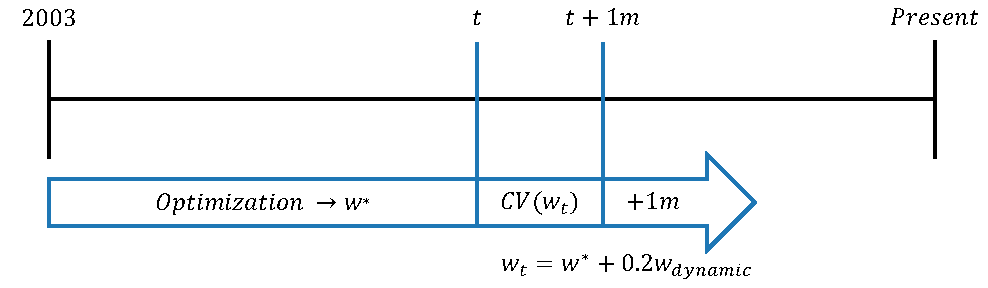
\includegraphics[width=\textwidth]{images/backtest_timeline.pdf}
    \end{center}
    \caption{\textbf{Iterative model performance validation methodology.}}
    \label{fig:backtest_timeline}
\end{figure}

The static threshold parameter $w^*$ itself is initially identified by evaluating a set of candidate values within the range $[0.6, 1.0]$ using incremental steps of $0.005$. For each threshold candidate, historical out-of-sample performance is evaluated to determine the combination yielding the highest product of market participation and active return. The threshold that maximizes this combined metric is chosen as the static threshold $w^*$.

This chapter established a comprehensive methodological framework for analyzing new issue premium in European investment-grade corporate bonds, progressing from data preprocessing through feature selection to model optimization and validation. The XGBoost-based approach, enhanced by ternary classification and hybrid threshold calibration, effectively captures complex relationships between bond characteristics and short-term performance. The resulting framework provides portfolio managers with a quantitative tool for systematic new issue evaluation, representing a significant advancement over traditional qualitative approaches and establishing the foundation for subsequent feature analysis and performance evaluation.
\chapter{Feature Research}
\label{ch:feature_research}

This chapter examines the determinants of NIP in EUR Investment Grade Corporate Bonds. The analysis identifies and evaluates features at both the microeconomic and macroeconomic levels that systematically predict the short-term outperformance of newly issued bonds. Building on established research in high-yield markets \parencite{Geerts2022PredictingYield}, this investigation adapts and extends these methodologies to the investment-grade segment, where the NIP phenomenon operates under different dynamics. Through rigorous statistical testing and feature importance measurements, a comprehensive set of predictive variables is developed to form the foundation of the predictive model. Statistical significance levels and detailed test results are provided in the Appendix Table \ref{tab:feature_t_statistics}.

\section{Microeconomic Features}

Microeconomic features capture bond-specific characteristics and issuer attributes that influence pricing dynamics and subsequent performance in the secondary market. These features reflect the fundamental risk-return properties of individual bonds and the information asymmetry between issuers and investors \parencite{Geerts2022PredictingYield}. The following sections analyze the most relevant microeconomic determinants of the new issue premium.

\subsection{First-Time Issuer}
Investors need to allocate research capacity to familiarize themselves with the risks and opportunities associated with first-time issuers. This additional effort often translates into a premium in the primary market. First-time issuers must compensate investors for the uncertainty and information asymmetry inherent in the absence of a trading history \parencite{Geerts2022PredictingYield}. Empirical evidence from the EUR investment-grade bond market confirms this hypothesis. When examining new issuances in a binary fashion (first-time vs. seasoned issuers), a significant first-time issuer premium emerges:

$$\text{FTI Premium} = E[XR]_{\text{first-time}} - E[XR]_{\text{seasoned}} \approx 34 \text{ basis points}$$

The strong contrast between the positive average excess return of first-time issuers (+23.94 bp) and the negative return of seasoned issuers (-10.23 bp) underscores the economic significance of this feature. Statistical analysis reveals strong significance at the 1\% level, confirming the robustness of the first-time issuer effect in predicting the new issue premium.

\begin{figure}[h]
    \begin{center}
        %% Creator: Matplotlib, PGF backend
%%
%% To include the figure in your LaTeX document, write
%%   \input{<filename>.pgf}
%%
%% Make sure the required packages are loaded in your preamble
%%   \usepackage{pgf}
%%
%% Also ensure that all the required font packages are loaded; for instance,
%% the lmodern package is sometimes necessary when using math font.
%%   \usepackage{lmodern}
%%
%% Figures using additional raster images can only be included by \input if
%% they are in the same directory as the main LaTeX file. For loading figures
%% from other directories you can use the `import` package
%%   \usepackage{import}
%%
%% and then include the figures with
%%   \import{<path to file>}{<filename>.pgf}
%%
%% Matplotlib used the following preamble
%%   \def\mathdefault#1{#1}
%%   \everymath=\expandafter{\the\everymath\displaystyle}
%%   \IfFileExists{scrextend.sty}{
%%     \usepackage[fontsize=10.000000pt]{scrextend}
%%   }{
%%     \renewcommand{\normalsize}{\fontsize{10.000000}{12.000000}\selectfont}
%%     \normalsize
%%   }
%%   \usepackage{amsmath}
%%   \usepackage{amssymb}
%%   \usepackage{mathpazo}
%%   \makeatletter\@ifpackageloaded{underscore}{}{\usepackage[strings]{underscore}}\makeatother
%%
\begingroup%
\makeatletter%
\begin{pgfpicture}%
\pgfpathrectangle{\pgfpointorigin}{\pgfqpoint{5.900000in}{2.000000in}}%
\pgfusepath{use as bounding box, clip}%
\begin{pgfscope}%
\pgfsetbuttcap%
\pgfsetmiterjoin%
\definecolor{currentfill}{rgb}{1.000000,1.000000,1.000000}%
\pgfsetfillcolor{currentfill}%
\pgfsetlinewidth{0.000000pt}%
\definecolor{currentstroke}{rgb}{1.000000,1.000000,1.000000}%
\pgfsetstrokecolor{currentstroke}%
\pgfsetdash{}{0pt}%
\pgfpathmoveto{\pgfqpoint{0.000000in}{0.000000in}}%
\pgfpathlineto{\pgfqpoint{5.900000in}{0.000000in}}%
\pgfpathlineto{\pgfqpoint{5.900000in}{2.000000in}}%
\pgfpathlineto{\pgfqpoint{0.000000in}{2.000000in}}%
\pgfpathlineto{\pgfqpoint{0.000000in}{0.000000in}}%
\pgfpathclose%
\pgfusepath{fill}%
\end{pgfscope}%
\begin{pgfscope}%
\pgfsetbuttcap%
\pgfsetmiterjoin%
\definecolor{currentfill}{rgb}{1.000000,1.000000,1.000000}%
\pgfsetfillcolor{currentfill}%
\pgfsetlinewidth{0.000000pt}%
\definecolor{currentstroke}{rgb}{0.000000,0.000000,0.000000}%
\pgfsetstrokecolor{currentstroke}%
\pgfsetstrokeopacity{0.000000}%
\pgfsetdash{}{0pt}%
\pgfpathmoveto{\pgfqpoint{0.737500in}{0.220000in}}%
\pgfpathlineto{\pgfqpoint{5.310000in}{0.220000in}}%
\pgfpathlineto{\pgfqpoint{5.310000in}{1.760000in}}%
\pgfpathlineto{\pgfqpoint{0.737500in}{1.760000in}}%
\pgfpathlineto{\pgfqpoint{0.737500in}{0.220000in}}%
\pgfpathclose%
\pgfusepath{fill}%
\end{pgfscope}%
\begin{pgfscope}%
\pgfpathrectangle{\pgfqpoint{0.737500in}{0.220000in}}{\pgfqpoint{4.572500in}{1.540000in}}%
\pgfusepath{clip}%
\pgfsetbuttcap%
\pgfsetmiterjoin%
\definecolor{currentfill}{rgb}{0.121569,0.466667,0.705882}%
\pgfsetfillcolor{currentfill}%
\pgfsetlinewidth{0.000000pt}%
\definecolor{currentstroke}{rgb}{0.000000,0.000000,0.000000}%
\pgfsetstrokecolor{currentstroke}%
\pgfsetstrokeopacity{0.000000}%
\pgfsetdash{}{0pt}%
\pgfpathmoveto{\pgfqpoint{0.945341in}{0.709106in}}%
\pgfpathlineto{\pgfqpoint{2.792816in}{0.709106in}}%
\pgfpathlineto{\pgfqpoint{2.792816in}{0.290000in}}%
\pgfpathlineto{\pgfqpoint{0.945341in}{0.290000in}}%
\pgfpathlineto{\pgfqpoint{0.945341in}{0.709106in}}%
\pgfpathclose%
\pgfusepath{fill}%
\end{pgfscope}%
\begin{pgfscope}%
\pgfpathrectangle{\pgfqpoint{0.737500in}{0.220000in}}{\pgfqpoint{4.572500in}{1.540000in}}%
\pgfusepath{clip}%
\pgfsetbuttcap%
\pgfsetmiterjoin%
\definecolor{currentfill}{rgb}{0.121569,0.466667,0.705882}%
\pgfsetfillcolor{currentfill}%
\pgfsetlinewidth{0.000000pt}%
\definecolor{currentstroke}{rgb}{0.000000,0.000000,0.000000}%
\pgfsetstrokecolor{currentstroke}%
\pgfsetstrokeopacity{0.000000}%
\pgfsetdash{}{0pt}%
\pgfpathmoveto{\pgfqpoint{3.254684in}{0.709106in}}%
\pgfpathlineto{\pgfqpoint{5.102159in}{0.709106in}}%
\pgfpathlineto{\pgfqpoint{5.102159in}{1.690000in}}%
\pgfpathlineto{\pgfqpoint{3.254684in}{1.690000in}}%
\pgfpathlineto{\pgfqpoint{3.254684in}{0.709106in}}%
\pgfpathclose%
\pgfusepath{fill}%
\end{pgfscope}%
\begin{pgfscope}%
\pgfsetbuttcap%
\pgfsetroundjoin%
\definecolor{currentfill}{rgb}{0.000000,0.000000,0.000000}%
\pgfsetfillcolor{currentfill}%
\pgfsetlinewidth{0.803000pt}%
\definecolor{currentstroke}{rgb}{0.000000,0.000000,0.000000}%
\pgfsetstrokecolor{currentstroke}%
\pgfsetdash{}{0pt}%
\pgfsys@defobject{currentmarker}{\pgfqpoint{0.000000in}{-0.048611in}}{\pgfqpoint{0.000000in}{0.000000in}}{%
\pgfpathmoveto{\pgfqpoint{0.000000in}{0.000000in}}%
\pgfpathlineto{\pgfqpoint{0.000000in}{-0.048611in}}%
\pgfusepath{stroke,fill}%
}%
\begin{pgfscope}%
\pgfsys@transformshift{1.869078in}{0.220000in}%
\pgfsys@useobject{currentmarker}{}%
\end{pgfscope}%
\end{pgfscope}%
\begin{pgfscope}%
\definecolor{textcolor}{rgb}{0.000000,0.000000,0.000000}%
\pgfsetstrokecolor{textcolor}%
\pgfsetfillcolor{textcolor}%
\pgftext[x=1.869078in,y=0.122778in,,top]{\color{textcolor}{\rmfamily\fontsize{10.000000}{12.000000}\selectfont\catcode`\^=\active\def^{\ifmmode\sp\else\^{}\fi}\catcode`\%=\active\def%{\%}Seasoned Issuer}}%
\end{pgfscope}%
\begin{pgfscope}%
\pgfsetbuttcap%
\pgfsetroundjoin%
\definecolor{currentfill}{rgb}{0.000000,0.000000,0.000000}%
\pgfsetfillcolor{currentfill}%
\pgfsetlinewidth{0.803000pt}%
\definecolor{currentstroke}{rgb}{0.000000,0.000000,0.000000}%
\pgfsetstrokecolor{currentstroke}%
\pgfsetdash{}{0pt}%
\pgfsys@defobject{currentmarker}{\pgfqpoint{0.000000in}{-0.048611in}}{\pgfqpoint{0.000000in}{0.000000in}}{%
\pgfpathmoveto{\pgfqpoint{0.000000in}{0.000000in}}%
\pgfpathlineto{\pgfqpoint{0.000000in}{-0.048611in}}%
\pgfusepath{stroke,fill}%
}%
\begin{pgfscope}%
\pgfsys@transformshift{4.178422in}{0.220000in}%
\pgfsys@useobject{currentmarker}{}%
\end{pgfscope}%
\end{pgfscope}%
\begin{pgfscope}%
\definecolor{textcolor}{rgb}{0.000000,0.000000,0.000000}%
\pgfsetstrokecolor{textcolor}%
\pgfsetfillcolor{textcolor}%
\pgftext[x=4.178422in,y=0.122778in,,top]{\color{textcolor}{\rmfamily\fontsize{10.000000}{12.000000}\selectfont\catcode`\^=\active\def^{\ifmmode\sp\else\^{}\fi}\catcode`\%=\active\def%{\%}First Time Issuer}}%
\end{pgfscope}%
\begin{pgfscope}%
\definecolor{textcolor}{rgb}{0.000000,0.000000,0.000000}%
\pgfsetstrokecolor{textcolor}%
\pgfsetfillcolor{textcolor}%
\pgftext[x=3.023750in,y=-0.073123in,,top]{\color{textcolor}{\rmfamily\fontsize{10.000000}{12.000000}\selectfont\catcode`\^=\active\def^{\ifmmode\sp\else\^{}\fi}\catcode`\%=\active\def%{\%}Issuer Type}}%
\end{pgfscope}%
\begin{pgfscope}%
\pgfsetbuttcap%
\pgfsetroundjoin%
\definecolor{currentfill}{rgb}{0.000000,0.000000,0.000000}%
\pgfsetfillcolor{currentfill}%
\pgfsetlinewidth{0.803000pt}%
\definecolor{currentstroke}{rgb}{0.000000,0.000000,0.000000}%
\pgfsetstrokecolor{currentstroke}%
\pgfsetdash{}{0pt}%
\pgfsys@defobject{currentmarker}{\pgfqpoint{-0.048611in}{0.000000in}}{\pgfqpoint{-0.000000in}{0.000000in}}{%
\pgfpathmoveto{\pgfqpoint{-0.000000in}{0.000000in}}%
\pgfpathlineto{\pgfqpoint{-0.048611in}{0.000000in}}%
\pgfusepath{stroke,fill}%
}%
\begin{pgfscope}%
\pgfsys@transformshift{0.737500in}{0.299335in}%
\pgfsys@useobject{currentmarker}{}%
\end{pgfscope}%
\end{pgfscope}%
\begin{pgfscope}%
\definecolor{textcolor}{rgb}{0.000000,0.000000,0.000000}%
\pgfsetstrokecolor{textcolor}%
\pgfsetfillcolor{textcolor}%
\pgftext[x=0.385418in, y=0.248745in, left, base]{\color{textcolor}{\rmfamily\fontsize{10.000000}{12.000000}\selectfont\catcode`\^=\active\def^{\ifmmode\sp\else\^{}\fi}\catcode`\%=\active\def%{\%}$\mathdefault{\ensuremath{-}10}$}}%
\end{pgfscope}%
\begin{pgfscope}%
\pgfsetbuttcap%
\pgfsetroundjoin%
\definecolor{currentfill}{rgb}{0.000000,0.000000,0.000000}%
\pgfsetfillcolor{currentfill}%
\pgfsetlinewidth{0.803000pt}%
\definecolor{currentstroke}{rgb}{0.000000,0.000000,0.000000}%
\pgfsetstrokecolor{currentstroke}%
\pgfsetdash{}{0pt}%
\pgfsys@defobject{currentmarker}{\pgfqpoint{-0.048611in}{0.000000in}}{\pgfqpoint{-0.000000in}{0.000000in}}{%
\pgfpathmoveto{\pgfqpoint{-0.000000in}{0.000000in}}%
\pgfpathlineto{\pgfqpoint{-0.048611in}{0.000000in}}%
\pgfusepath{stroke,fill}%
}%
\begin{pgfscope}%
\pgfsys@transformshift{0.737500in}{0.709106in}%
\pgfsys@useobject{currentmarker}{}%
\end{pgfscope}%
\end{pgfscope}%
\begin{pgfscope}%
\definecolor{textcolor}{rgb}{0.000000,0.000000,0.000000}%
\pgfsetstrokecolor{textcolor}%
\pgfsetfillcolor{textcolor}%
\pgftext[x=0.570833in, y=0.658516in, left, base]{\color{textcolor}{\rmfamily\fontsize{10.000000}{12.000000}\selectfont\catcode`\^=\active\def^{\ifmmode\sp\else\^{}\fi}\catcode`\%=\active\def%{\%}$\mathdefault{0}$}}%
\end{pgfscope}%
\begin{pgfscope}%
\pgfsetbuttcap%
\pgfsetroundjoin%
\definecolor{currentfill}{rgb}{0.000000,0.000000,0.000000}%
\pgfsetfillcolor{currentfill}%
\pgfsetlinewidth{0.803000pt}%
\definecolor{currentstroke}{rgb}{0.000000,0.000000,0.000000}%
\pgfsetstrokecolor{currentstroke}%
\pgfsetdash{}{0pt}%
\pgfsys@defobject{currentmarker}{\pgfqpoint{-0.048611in}{0.000000in}}{\pgfqpoint{-0.000000in}{0.000000in}}{%
\pgfpathmoveto{\pgfqpoint{-0.000000in}{0.000000in}}%
\pgfpathlineto{\pgfqpoint{-0.048611in}{0.000000in}}%
\pgfusepath{stroke,fill}%
}%
\begin{pgfscope}%
\pgfsys@transformshift{0.737500in}{1.118877in}%
\pgfsys@useobject{currentmarker}{}%
\end{pgfscope}%
\end{pgfscope}%
\begin{pgfscope}%
\definecolor{textcolor}{rgb}{0.000000,0.000000,0.000000}%
\pgfsetstrokecolor{textcolor}%
\pgfsetfillcolor{textcolor}%
\pgftext[x=0.501389in, y=1.068287in, left, base]{\color{textcolor}{\rmfamily\fontsize{10.000000}{12.000000}\selectfont\catcode`\^=\active\def^{\ifmmode\sp\else\^{}\fi}\catcode`\%=\active\def%{\%}$\mathdefault{10}$}}%
\end{pgfscope}%
\begin{pgfscope}%
\pgfsetbuttcap%
\pgfsetroundjoin%
\definecolor{currentfill}{rgb}{0.000000,0.000000,0.000000}%
\pgfsetfillcolor{currentfill}%
\pgfsetlinewidth{0.803000pt}%
\definecolor{currentstroke}{rgb}{0.000000,0.000000,0.000000}%
\pgfsetstrokecolor{currentstroke}%
\pgfsetdash{}{0pt}%
\pgfsys@defobject{currentmarker}{\pgfqpoint{-0.048611in}{0.000000in}}{\pgfqpoint{-0.000000in}{0.000000in}}{%
\pgfpathmoveto{\pgfqpoint{-0.000000in}{0.000000in}}%
\pgfpathlineto{\pgfqpoint{-0.048611in}{0.000000in}}%
\pgfusepath{stroke,fill}%
}%
\begin{pgfscope}%
\pgfsys@transformshift{0.737500in}{1.528648in}%
\pgfsys@useobject{currentmarker}{}%
\end{pgfscope}%
\end{pgfscope}%
\begin{pgfscope}%
\definecolor{textcolor}{rgb}{0.000000,0.000000,0.000000}%
\pgfsetstrokecolor{textcolor}%
\pgfsetfillcolor{textcolor}%
\pgftext[x=0.501389in, y=1.478058in, left, base]{\color{textcolor}{\rmfamily\fontsize{10.000000}{12.000000}\selectfont\catcode`\^=\active\def^{\ifmmode\sp\else\^{}\fi}\catcode`\%=\active\def%{\%}$\mathdefault{20}$}}%
\end{pgfscope}%
\begin{pgfscope}%
\definecolor{textcolor}{rgb}{0.000000,0.000000,0.000000}%
\pgfsetstrokecolor{textcolor}%
\pgfsetfillcolor{textcolor}%
\pgftext[x=0.329863in,y=0.990000in,,bottom,rotate=90.000000]{\color{textcolor}{\rmfamily\fontsize{10.000000}{12.000000}\selectfont\catcode`\^=\active\def^{\ifmmode\sp\else\^{}\fi}\catcode`\%=\active\def%{\%}E[xr] (bp)}}%
\end{pgfscope}%
\begin{pgfscope}%
\pgfsetrectcap%
\pgfsetmiterjoin%
\pgfsetlinewidth{0.803000pt}%
\definecolor{currentstroke}{rgb}{0.000000,0.000000,0.000000}%
\pgfsetstrokecolor{currentstroke}%
\pgfsetdash{}{0pt}%
\pgfpathmoveto{\pgfqpoint{0.737500in}{0.220000in}}%
\pgfpathlineto{\pgfqpoint{0.737500in}{1.760000in}}%
\pgfusepath{stroke}%
\end{pgfscope}%
\begin{pgfscope}%
\pgfsetrectcap%
\pgfsetmiterjoin%
\pgfsetlinewidth{0.803000pt}%
\definecolor{currentstroke}{rgb}{0.000000,0.000000,0.000000}%
\pgfsetstrokecolor{currentstroke}%
\pgfsetdash{}{0pt}%
\pgfpathmoveto{\pgfqpoint{5.310000in}{0.220000in}}%
\pgfpathlineto{\pgfqpoint{5.310000in}{1.760000in}}%
\pgfusepath{stroke}%
\end{pgfscope}%
\begin{pgfscope}%
\pgfsetrectcap%
\pgfsetmiterjoin%
\pgfsetlinewidth{0.803000pt}%
\definecolor{currentstroke}{rgb}{0.000000,0.000000,0.000000}%
\pgfsetstrokecolor{currentstroke}%
\pgfsetdash{}{0pt}%
\pgfpathmoveto{\pgfqpoint{0.737500in}{0.220000in}}%
\pgfpathlineto{\pgfqpoint{5.310000in}{0.220000in}}%
\pgfusepath{stroke}%
\end{pgfscope}%
\begin{pgfscope}%
\pgfsetrectcap%
\pgfsetmiterjoin%
\pgfsetlinewidth{0.803000pt}%
\definecolor{currentstroke}{rgb}{0.000000,0.000000,0.000000}%
\pgfsetstrokecolor{currentstroke}%
\pgfsetdash{}{0pt}%
\pgfpathmoveto{\pgfqpoint{0.737500in}{1.760000in}}%
\pgfpathlineto{\pgfqpoint{5.310000in}{1.760000in}}%
\pgfusepath{stroke}%
\end{pgfscope}%
\end{pgfpicture}%
\makeatother%
\endgroup%

    \end{center}
    \caption{Expected Excess Returns by Issuer Type: Comparison of First-Time Versus Seasoned Issuers}
    \label{fig:fti}
\end{figure}

\subsection{Credit Risk Indicators}

\subsubsection{Coupon}
The coupon rate represents both the periodic interest payment to bondholders and serves as a proxy for credit risk. Higher coupons often signal elevated risk profiles, limiting the potential investor base \parencite{Geerts2022PredictingYield}. The relationship between coupon rates and excess returns was found to be statistically significant at the 5\% level. Interestingly, the relationship does not appear strictly monotonic when analyzed categorically. Bonds in the lowest- and highest-coupon quintiles tend to outperform those in middle quintiles. This nonlinear pattern suggests that factors beyond simple risk compensation may be at play, possibly including liquidity considerations or market segmentation effects.

\subsubsection{Z-Spread}
The Z-spread represents the constant yield spread over the zero-coupon Treasury yield curve required to discount a bond's cash flows to match its current market price. It provides a more comprehensive risk assessment than nominal spreads by accounting for the entire payment structure of the bond between different maturities \parencite[pp. 816 - 818]{Fabozzi2021TheEdition}. Due to the inconsistent availability of Z-spread data, an approximation was used:

$$Z \approx I = \text{YTM} - s_T$$

Where $I$ is the I-spread, YTM is the yield to maturity and $s_T$ is the linearly interpolated swap rate based on maturity. The yield to maturity itself was approximated as:

\begin{align}
\text{ytm} &\approx \frac{2(c+ \frac{100-p}{T})}{100+p} \\
\text{where} \quad p &: \text{Issue price} \nonumber\\
c &: \text{Coupon} \nonumber\\
T &: \text{Maturity} \nonumber
\end{align}

Two derived Z-spread features were analyzed:

\begin{enumerate}
    \item Z-spread rank among sector peers
    \item Distance to benchmark spread curve, defined as:
    $$\Delta Z = Z - Z_B(d)$$
    where $d$ is the estimated spread duration
\end{enumerate}

The Z-spread feature demonstrated strong statistical significance at the 1\% level, with the Z-spread ranked in sector also showing significance. The spread premium exhibits an interesting pattern when plotted against excess returns by quintiles. Bonds in the middle (third) quintile showed the highest excess returns (+8.87 bp), while those in the lowest quintile significantly underperformed (-25.32 bp).

\begin{figure}[h]
    \begin{center}
        %% Creator: Matplotlib, PGF backend
%%
%% To include the figure in your LaTeX document, write
%%   \input{<filename>.pgf}
%%
%% Make sure the required packages are loaded in your preamble
%%   \usepackage{pgf}
%%
%% Also ensure that all the required font packages are loaded; for instance,
%% the lmodern package is sometimes necessary when using math font.
%%   \usepackage{lmodern}
%%
%% Figures using additional raster images can only be included by \input if
%% they are in the same directory as the main LaTeX file. For loading figures
%% from other directories you can use the `import` package
%%   \usepackage{import}
%%
%% and then include the figures with
%%   \import{<path to file>}{<filename>.pgf}
%%
%% Matplotlib used the following preamble
%%   \def\mathdefault#1{#1}
%%   \everymath=\expandafter{\the\everymath\displaystyle}
%%   \IfFileExists{scrextend.sty}{
%%     \usepackage[fontsize=10.000000pt]{scrextend}
%%   }{
%%     \renewcommand{\normalsize}{\fontsize{10.000000}{12.000000}\selectfont}
%%     \normalsize
%%   }
%%   \usepackage{amsmath}
%%   \usepackage{amssymb}
%%   \usepackage{mathpazo}
%%   \makeatletter\@ifpackageloaded{underscore}{}{\usepackage[strings]{underscore}}\makeatother
%%
\begingroup%
\makeatletter%
\begin{pgfpicture}%
\pgfpathrectangle{\pgfpointorigin}{\pgfqpoint{5.900000in}{2.000000in}}%
\pgfusepath{use as bounding box, clip}%
\begin{pgfscope}%
\pgfsetbuttcap%
\pgfsetmiterjoin%
\definecolor{currentfill}{rgb}{1.000000,1.000000,1.000000}%
\pgfsetfillcolor{currentfill}%
\pgfsetlinewidth{0.000000pt}%
\definecolor{currentstroke}{rgb}{1.000000,1.000000,1.000000}%
\pgfsetstrokecolor{currentstroke}%
\pgfsetdash{}{0pt}%
\pgfpathmoveto{\pgfqpoint{0.000000in}{0.000000in}}%
\pgfpathlineto{\pgfqpoint{5.900000in}{0.000000in}}%
\pgfpathlineto{\pgfqpoint{5.900000in}{2.000000in}}%
\pgfpathlineto{\pgfqpoint{0.000000in}{2.000000in}}%
\pgfpathlineto{\pgfqpoint{0.000000in}{0.000000in}}%
\pgfpathclose%
\pgfusepath{fill}%
\end{pgfscope}%
\begin{pgfscope}%
\pgfsetbuttcap%
\pgfsetmiterjoin%
\definecolor{currentfill}{rgb}{1.000000,1.000000,1.000000}%
\pgfsetfillcolor{currentfill}%
\pgfsetlinewidth{0.000000pt}%
\definecolor{currentstroke}{rgb}{0.000000,0.000000,0.000000}%
\pgfsetstrokecolor{currentstroke}%
\pgfsetstrokeopacity{0.000000}%
\pgfsetdash{}{0pt}%
\pgfpathmoveto{\pgfqpoint{0.737500in}{0.220000in}}%
\pgfpathlineto{\pgfqpoint{5.310000in}{0.220000in}}%
\pgfpathlineto{\pgfqpoint{5.310000in}{1.760000in}}%
\pgfpathlineto{\pgfqpoint{0.737500in}{1.760000in}}%
\pgfpathlineto{\pgfqpoint{0.737500in}{0.220000in}}%
\pgfpathclose%
\pgfusepath{fill}%
\end{pgfscope}%
\begin{pgfscope}%
\pgfpathrectangle{\pgfqpoint{0.737500in}{0.220000in}}{\pgfqpoint{4.572500in}{1.540000in}}%
\pgfusepath{clip}%
\pgfsetbuttcap%
\pgfsetmiterjoin%
\definecolor{currentfill}{rgb}{0.121569,0.466667,0.705882}%
\pgfsetfillcolor{currentfill}%
\pgfsetlinewidth{0.000000pt}%
\definecolor{currentstroke}{rgb}{0.000000,0.000000,0.000000}%
\pgfsetstrokecolor{currentstroke}%
\pgfsetstrokeopacity{0.000000}%
\pgfsetdash{}{0pt}%
\pgfpathmoveto{\pgfqpoint{0.945341in}{1.326894in}}%
\pgfpathlineto{\pgfqpoint{1.638144in}{1.326894in}}%
\pgfpathlineto{\pgfqpoint{1.638144in}{0.290000in}}%
\pgfpathlineto{\pgfqpoint{0.945341in}{0.290000in}}%
\pgfpathlineto{\pgfqpoint{0.945341in}{1.326894in}}%
\pgfpathclose%
\pgfusepath{fill}%
\end{pgfscope}%
\begin{pgfscope}%
\pgfpathrectangle{\pgfqpoint{0.737500in}{0.220000in}}{\pgfqpoint{4.572500in}{1.540000in}}%
\pgfusepath{clip}%
\pgfsetbuttcap%
\pgfsetmiterjoin%
\definecolor{currentfill}{rgb}{0.121569,0.466667,0.705882}%
\pgfsetfillcolor{currentfill}%
\pgfsetlinewidth{0.000000pt}%
\definecolor{currentstroke}{rgb}{0.000000,0.000000,0.000000}%
\pgfsetstrokecolor{currentstroke}%
\pgfsetstrokeopacity{0.000000}%
\pgfsetdash{}{0pt}%
\pgfpathmoveto{\pgfqpoint{1.811345in}{1.326894in}}%
\pgfpathlineto{\pgfqpoint{2.504148in}{1.326894in}}%
\pgfpathlineto{\pgfqpoint{2.504148in}{0.668120in}}%
\pgfpathlineto{\pgfqpoint{1.811345in}{0.668120in}}%
\pgfpathlineto{\pgfqpoint{1.811345in}{1.326894in}}%
\pgfpathclose%
\pgfusepath{fill}%
\end{pgfscope}%
\begin{pgfscope}%
\pgfpathrectangle{\pgfqpoint{0.737500in}{0.220000in}}{\pgfqpoint{4.572500in}{1.540000in}}%
\pgfusepath{clip}%
\pgfsetbuttcap%
\pgfsetmiterjoin%
\definecolor{currentfill}{rgb}{0.121569,0.466667,0.705882}%
\pgfsetfillcolor{currentfill}%
\pgfsetlinewidth{0.000000pt}%
\definecolor{currentstroke}{rgb}{0.000000,0.000000,0.000000}%
\pgfsetstrokecolor{currentstroke}%
\pgfsetstrokeopacity{0.000000}%
\pgfsetdash{}{0pt}%
\pgfpathmoveto{\pgfqpoint{2.677348in}{1.326894in}}%
\pgfpathlineto{\pgfqpoint{3.370152in}{1.326894in}}%
\pgfpathlineto{\pgfqpoint{3.370152in}{1.690000in}}%
\pgfpathlineto{\pgfqpoint{2.677348in}{1.690000in}}%
\pgfpathlineto{\pgfqpoint{2.677348in}{1.326894in}}%
\pgfpathclose%
\pgfusepath{fill}%
\end{pgfscope}%
\begin{pgfscope}%
\pgfpathrectangle{\pgfqpoint{0.737500in}{0.220000in}}{\pgfqpoint{4.572500in}{1.540000in}}%
\pgfusepath{clip}%
\pgfsetbuttcap%
\pgfsetmiterjoin%
\definecolor{currentfill}{rgb}{0.121569,0.466667,0.705882}%
\pgfsetfillcolor{currentfill}%
\pgfsetlinewidth{0.000000pt}%
\definecolor{currentstroke}{rgb}{0.000000,0.000000,0.000000}%
\pgfsetstrokecolor{currentstroke}%
\pgfsetstrokeopacity{0.000000}%
\pgfsetdash{}{0pt}%
\pgfpathmoveto{\pgfqpoint{3.543352in}{1.326894in}}%
\pgfpathlineto{\pgfqpoint{4.236155in}{1.326894in}}%
\pgfpathlineto{\pgfqpoint{4.236155in}{1.125643in}}%
\pgfpathlineto{\pgfqpoint{3.543352in}{1.125643in}}%
\pgfpathlineto{\pgfqpoint{3.543352in}{1.326894in}}%
\pgfpathclose%
\pgfusepath{fill}%
\end{pgfscope}%
\begin{pgfscope}%
\pgfpathrectangle{\pgfqpoint{0.737500in}{0.220000in}}{\pgfqpoint{4.572500in}{1.540000in}}%
\pgfusepath{clip}%
\pgfsetbuttcap%
\pgfsetmiterjoin%
\definecolor{currentfill}{rgb}{0.121569,0.466667,0.705882}%
\pgfsetfillcolor{currentfill}%
\pgfsetlinewidth{0.000000pt}%
\definecolor{currentstroke}{rgb}{0.000000,0.000000,0.000000}%
\pgfsetstrokecolor{currentstroke}%
\pgfsetstrokeopacity{0.000000}%
\pgfsetdash{}{0pt}%
\pgfpathmoveto{\pgfqpoint{4.409356in}{1.326894in}}%
\pgfpathlineto{\pgfqpoint{5.102159in}{1.326894in}}%
\pgfpathlineto{\pgfqpoint{5.102159in}{1.260851in}}%
\pgfpathlineto{\pgfqpoint{4.409356in}{1.260851in}}%
\pgfpathlineto{\pgfqpoint{4.409356in}{1.326894in}}%
\pgfpathclose%
\pgfusepath{fill}%
\end{pgfscope}%
\begin{pgfscope}%
\pgfsetbuttcap%
\pgfsetroundjoin%
\definecolor{currentfill}{rgb}{0.000000,0.000000,0.000000}%
\pgfsetfillcolor{currentfill}%
\pgfsetlinewidth{0.803000pt}%
\definecolor{currentstroke}{rgb}{0.000000,0.000000,0.000000}%
\pgfsetstrokecolor{currentstroke}%
\pgfsetdash{}{0pt}%
\pgfsys@defobject{currentmarker}{\pgfqpoint{0.000000in}{-0.048611in}}{\pgfqpoint{0.000000in}{0.000000in}}{%
\pgfpathmoveto{\pgfqpoint{0.000000in}{0.000000in}}%
\pgfpathlineto{\pgfqpoint{0.000000in}{-0.048611in}}%
\pgfusepath{stroke,fill}%
}%
\begin{pgfscope}%
\pgfsys@transformshift{1.291742in}{0.220000in}%
\pgfsys@useobject{currentmarker}{}%
\end{pgfscope}%
\end{pgfscope}%
\begin{pgfscope}%
\definecolor{textcolor}{rgb}{0.000000,0.000000,0.000000}%
\pgfsetstrokecolor{textcolor}%
\pgfsetfillcolor{textcolor}%
\pgftext[x=1.291742in,y=0.122778in,,top]{\color{textcolor}{\rmfamily\fontsize{10.000000}{12.000000}\selectfont\catcode`\^=\active\def^{\ifmmode\sp\else\^{}\fi}\catcode`\%=\active\def%{\%}$\mathdefault{1}$}}%
\end{pgfscope}%
\begin{pgfscope}%
\pgfsetbuttcap%
\pgfsetroundjoin%
\definecolor{currentfill}{rgb}{0.000000,0.000000,0.000000}%
\pgfsetfillcolor{currentfill}%
\pgfsetlinewidth{0.803000pt}%
\definecolor{currentstroke}{rgb}{0.000000,0.000000,0.000000}%
\pgfsetstrokecolor{currentstroke}%
\pgfsetdash{}{0pt}%
\pgfsys@defobject{currentmarker}{\pgfqpoint{0.000000in}{-0.048611in}}{\pgfqpoint{0.000000in}{0.000000in}}{%
\pgfpathmoveto{\pgfqpoint{0.000000in}{0.000000in}}%
\pgfpathlineto{\pgfqpoint{0.000000in}{-0.048611in}}%
\pgfusepath{stroke,fill}%
}%
\begin{pgfscope}%
\pgfsys@transformshift{2.157746in}{0.220000in}%
\pgfsys@useobject{currentmarker}{}%
\end{pgfscope}%
\end{pgfscope}%
\begin{pgfscope}%
\definecolor{textcolor}{rgb}{0.000000,0.000000,0.000000}%
\pgfsetstrokecolor{textcolor}%
\pgfsetfillcolor{textcolor}%
\pgftext[x=2.157746in,y=0.122778in,,top]{\color{textcolor}{\rmfamily\fontsize{10.000000}{12.000000}\selectfont\catcode`\^=\active\def^{\ifmmode\sp\else\^{}\fi}\catcode`\%=\active\def%{\%}$\mathdefault{2}$}}%
\end{pgfscope}%
\begin{pgfscope}%
\pgfsetbuttcap%
\pgfsetroundjoin%
\definecolor{currentfill}{rgb}{0.000000,0.000000,0.000000}%
\pgfsetfillcolor{currentfill}%
\pgfsetlinewidth{0.803000pt}%
\definecolor{currentstroke}{rgb}{0.000000,0.000000,0.000000}%
\pgfsetstrokecolor{currentstroke}%
\pgfsetdash{}{0pt}%
\pgfsys@defobject{currentmarker}{\pgfqpoint{0.000000in}{-0.048611in}}{\pgfqpoint{0.000000in}{0.000000in}}{%
\pgfpathmoveto{\pgfqpoint{0.000000in}{0.000000in}}%
\pgfpathlineto{\pgfqpoint{0.000000in}{-0.048611in}}%
\pgfusepath{stroke,fill}%
}%
\begin{pgfscope}%
\pgfsys@transformshift{3.023750in}{0.220000in}%
\pgfsys@useobject{currentmarker}{}%
\end{pgfscope}%
\end{pgfscope}%
\begin{pgfscope}%
\definecolor{textcolor}{rgb}{0.000000,0.000000,0.000000}%
\pgfsetstrokecolor{textcolor}%
\pgfsetfillcolor{textcolor}%
\pgftext[x=3.023750in,y=0.122778in,,top]{\color{textcolor}{\rmfamily\fontsize{10.000000}{12.000000}\selectfont\catcode`\^=\active\def^{\ifmmode\sp\else\^{}\fi}\catcode`\%=\active\def%{\%}$\mathdefault{3}$}}%
\end{pgfscope}%
\begin{pgfscope}%
\pgfsetbuttcap%
\pgfsetroundjoin%
\definecolor{currentfill}{rgb}{0.000000,0.000000,0.000000}%
\pgfsetfillcolor{currentfill}%
\pgfsetlinewidth{0.803000pt}%
\definecolor{currentstroke}{rgb}{0.000000,0.000000,0.000000}%
\pgfsetstrokecolor{currentstroke}%
\pgfsetdash{}{0pt}%
\pgfsys@defobject{currentmarker}{\pgfqpoint{0.000000in}{-0.048611in}}{\pgfqpoint{0.000000in}{0.000000in}}{%
\pgfpathmoveto{\pgfqpoint{0.000000in}{0.000000in}}%
\pgfpathlineto{\pgfqpoint{0.000000in}{-0.048611in}}%
\pgfusepath{stroke,fill}%
}%
\begin{pgfscope}%
\pgfsys@transformshift{3.889754in}{0.220000in}%
\pgfsys@useobject{currentmarker}{}%
\end{pgfscope}%
\end{pgfscope}%
\begin{pgfscope}%
\definecolor{textcolor}{rgb}{0.000000,0.000000,0.000000}%
\pgfsetstrokecolor{textcolor}%
\pgfsetfillcolor{textcolor}%
\pgftext[x=3.889754in,y=0.122778in,,top]{\color{textcolor}{\rmfamily\fontsize{10.000000}{12.000000}\selectfont\catcode`\^=\active\def^{\ifmmode\sp\else\^{}\fi}\catcode`\%=\active\def%{\%}$\mathdefault{4}$}}%
\end{pgfscope}%
\begin{pgfscope}%
\pgfsetbuttcap%
\pgfsetroundjoin%
\definecolor{currentfill}{rgb}{0.000000,0.000000,0.000000}%
\pgfsetfillcolor{currentfill}%
\pgfsetlinewidth{0.803000pt}%
\definecolor{currentstroke}{rgb}{0.000000,0.000000,0.000000}%
\pgfsetstrokecolor{currentstroke}%
\pgfsetdash{}{0pt}%
\pgfsys@defobject{currentmarker}{\pgfqpoint{0.000000in}{-0.048611in}}{\pgfqpoint{0.000000in}{0.000000in}}{%
\pgfpathmoveto{\pgfqpoint{0.000000in}{0.000000in}}%
\pgfpathlineto{\pgfqpoint{0.000000in}{-0.048611in}}%
\pgfusepath{stroke,fill}%
}%
\begin{pgfscope}%
\pgfsys@transformshift{4.755758in}{0.220000in}%
\pgfsys@useobject{currentmarker}{}%
\end{pgfscope}%
\end{pgfscope}%
\begin{pgfscope}%
\definecolor{textcolor}{rgb}{0.000000,0.000000,0.000000}%
\pgfsetstrokecolor{textcolor}%
\pgfsetfillcolor{textcolor}%
\pgftext[x=4.755758in,y=0.122778in,,top]{\color{textcolor}{\rmfamily\fontsize{10.000000}{12.000000}\selectfont\catcode`\^=\active\def^{\ifmmode\sp\else\^{}\fi}\catcode`\%=\active\def%{\%}$\mathdefault{5}$}}%
\end{pgfscope}%
\begin{pgfscope}%
\definecolor{textcolor}{rgb}{0.000000,0.000000,0.000000}%
\pgfsetstrokecolor{textcolor}%
\pgfsetfillcolor{textcolor}%
\pgftext[x=3.023750in,y=-0.073123in,,top]{\color{textcolor}{\rmfamily\fontsize{10.000000}{12.000000}\selectfont\catcode`\^=\active\def^{\ifmmode\sp\else\^{}\fi}\catcode`\%=\active\def%{\%}Z-spread distance quintile}}%
\end{pgfscope}%
\begin{pgfscope}%
\pgfsetbuttcap%
\pgfsetroundjoin%
\definecolor{currentfill}{rgb}{0.000000,0.000000,0.000000}%
\pgfsetfillcolor{currentfill}%
\pgfsetlinewidth{0.803000pt}%
\definecolor{currentstroke}{rgb}{0.000000,0.000000,0.000000}%
\pgfsetstrokecolor{currentstroke}%
\pgfsetdash{}{0pt}%
\pgfsys@defobject{currentmarker}{\pgfqpoint{-0.048611in}{0.000000in}}{\pgfqpoint{-0.000000in}{0.000000in}}{%
\pgfpathmoveto{\pgfqpoint{-0.000000in}{0.000000in}}%
\pgfpathlineto{\pgfqpoint{-0.048611in}{0.000000in}}%
\pgfusepath{stroke,fill}%
}%
\begin{pgfscope}%
\pgfsys@transformshift{0.737500in}{0.507819in}%
\pgfsys@useobject{currentmarker}{}%
\end{pgfscope}%
\end{pgfscope}%
\begin{pgfscope}%
\definecolor{textcolor}{rgb}{0.000000,0.000000,0.000000}%
\pgfsetstrokecolor{textcolor}%
\pgfsetfillcolor{textcolor}%
\pgftext[x=0.385418in, y=0.457230in, left, base]{\color{textcolor}{\rmfamily\fontsize{10.000000}{12.000000}\selectfont\catcode`\^=\active\def^{\ifmmode\sp\else\^{}\fi}\catcode`\%=\active\def%{\%}$\mathdefault{\ensuremath{-}20}$}}%
\end{pgfscope}%
\begin{pgfscope}%
\pgfsetbuttcap%
\pgfsetroundjoin%
\definecolor{currentfill}{rgb}{0.000000,0.000000,0.000000}%
\pgfsetfillcolor{currentfill}%
\pgfsetlinewidth{0.803000pt}%
\definecolor{currentstroke}{rgb}{0.000000,0.000000,0.000000}%
\pgfsetstrokecolor{currentstroke}%
\pgfsetdash{}{0pt}%
\pgfsys@defobject{currentmarker}{\pgfqpoint{-0.048611in}{0.000000in}}{\pgfqpoint{-0.000000in}{0.000000in}}{%
\pgfpathmoveto{\pgfqpoint{-0.000000in}{0.000000in}}%
\pgfpathlineto{\pgfqpoint{-0.048611in}{0.000000in}}%
\pgfusepath{stroke,fill}%
}%
\begin{pgfscope}%
\pgfsys@transformshift{0.737500in}{0.917357in}%
\pgfsys@useobject{currentmarker}{}%
\end{pgfscope}%
\end{pgfscope}%
\begin{pgfscope}%
\definecolor{textcolor}{rgb}{0.000000,0.000000,0.000000}%
\pgfsetstrokecolor{textcolor}%
\pgfsetfillcolor{textcolor}%
\pgftext[x=0.385418in, y=0.866767in, left, base]{\color{textcolor}{\rmfamily\fontsize{10.000000}{12.000000}\selectfont\catcode`\^=\active\def^{\ifmmode\sp\else\^{}\fi}\catcode`\%=\active\def%{\%}$\mathdefault{\ensuremath{-}10}$}}%
\end{pgfscope}%
\begin{pgfscope}%
\pgfsetbuttcap%
\pgfsetroundjoin%
\definecolor{currentfill}{rgb}{0.000000,0.000000,0.000000}%
\pgfsetfillcolor{currentfill}%
\pgfsetlinewidth{0.803000pt}%
\definecolor{currentstroke}{rgb}{0.000000,0.000000,0.000000}%
\pgfsetstrokecolor{currentstroke}%
\pgfsetdash{}{0pt}%
\pgfsys@defobject{currentmarker}{\pgfqpoint{-0.048611in}{0.000000in}}{\pgfqpoint{-0.000000in}{0.000000in}}{%
\pgfpathmoveto{\pgfqpoint{-0.000000in}{0.000000in}}%
\pgfpathlineto{\pgfqpoint{-0.048611in}{0.000000in}}%
\pgfusepath{stroke,fill}%
}%
\begin{pgfscope}%
\pgfsys@transformshift{0.737500in}{1.326894in}%
\pgfsys@useobject{currentmarker}{}%
\end{pgfscope}%
\end{pgfscope}%
\begin{pgfscope}%
\definecolor{textcolor}{rgb}{0.000000,0.000000,0.000000}%
\pgfsetstrokecolor{textcolor}%
\pgfsetfillcolor{textcolor}%
\pgftext[x=0.570833in, y=1.276305in, left, base]{\color{textcolor}{\rmfamily\fontsize{10.000000}{12.000000}\selectfont\catcode`\^=\active\def^{\ifmmode\sp\else\^{}\fi}\catcode`\%=\active\def%{\%}$\mathdefault{0}$}}%
\end{pgfscope}%
\begin{pgfscope}%
\pgfsetbuttcap%
\pgfsetroundjoin%
\definecolor{currentfill}{rgb}{0.000000,0.000000,0.000000}%
\pgfsetfillcolor{currentfill}%
\pgfsetlinewidth{0.803000pt}%
\definecolor{currentstroke}{rgb}{0.000000,0.000000,0.000000}%
\pgfsetstrokecolor{currentstroke}%
\pgfsetdash{}{0pt}%
\pgfsys@defobject{currentmarker}{\pgfqpoint{-0.048611in}{0.000000in}}{\pgfqpoint{-0.000000in}{0.000000in}}{%
\pgfpathmoveto{\pgfqpoint{-0.000000in}{0.000000in}}%
\pgfpathlineto{\pgfqpoint{-0.048611in}{0.000000in}}%
\pgfusepath{stroke,fill}%
}%
\begin{pgfscope}%
\pgfsys@transformshift{0.737500in}{1.736432in}%
\pgfsys@useobject{currentmarker}{}%
\end{pgfscope}%
\end{pgfscope}%
\begin{pgfscope}%
\definecolor{textcolor}{rgb}{0.000000,0.000000,0.000000}%
\pgfsetstrokecolor{textcolor}%
\pgfsetfillcolor{textcolor}%
\pgftext[x=0.501389in, y=1.685842in, left, base]{\color{textcolor}{\rmfamily\fontsize{10.000000}{12.000000}\selectfont\catcode`\^=\active\def^{\ifmmode\sp\else\^{}\fi}\catcode`\%=\active\def%{\%}$\mathdefault{10}$}}%
\end{pgfscope}%
\begin{pgfscope}%
\definecolor{textcolor}{rgb}{0.000000,0.000000,0.000000}%
\pgfsetstrokecolor{textcolor}%
\pgfsetfillcolor{textcolor}%
\pgftext[x=0.329863in,y=0.990000in,,bottom,rotate=90.000000]{\color{textcolor}{\rmfamily\fontsize{10.000000}{12.000000}\selectfont\catcode`\^=\active\def^{\ifmmode\sp\else\^{}\fi}\catcode`\%=\active\def%{\%}E[xr] (bp)}}%
\end{pgfscope}%
\begin{pgfscope}%
\pgfsetrectcap%
\pgfsetmiterjoin%
\pgfsetlinewidth{0.803000pt}%
\definecolor{currentstroke}{rgb}{0.000000,0.000000,0.000000}%
\pgfsetstrokecolor{currentstroke}%
\pgfsetdash{}{0pt}%
\pgfpathmoveto{\pgfqpoint{0.737500in}{0.220000in}}%
\pgfpathlineto{\pgfqpoint{0.737500in}{1.760000in}}%
\pgfusepath{stroke}%
\end{pgfscope}%
\begin{pgfscope}%
\pgfsetrectcap%
\pgfsetmiterjoin%
\pgfsetlinewidth{0.803000pt}%
\definecolor{currentstroke}{rgb}{0.000000,0.000000,0.000000}%
\pgfsetstrokecolor{currentstroke}%
\pgfsetdash{}{0pt}%
\pgfpathmoveto{\pgfqpoint{5.310000in}{0.220000in}}%
\pgfpathlineto{\pgfqpoint{5.310000in}{1.760000in}}%
\pgfusepath{stroke}%
\end{pgfscope}%
\begin{pgfscope}%
\pgfsetrectcap%
\pgfsetmiterjoin%
\pgfsetlinewidth{0.803000pt}%
\definecolor{currentstroke}{rgb}{0.000000,0.000000,0.000000}%
\pgfsetstrokecolor{currentstroke}%
\pgfsetdash{}{0pt}%
\pgfpathmoveto{\pgfqpoint{0.737500in}{0.220000in}}%
\pgfpathlineto{\pgfqpoint{5.310000in}{0.220000in}}%
\pgfusepath{stroke}%
\end{pgfscope}%
\begin{pgfscope}%
\pgfsetrectcap%
\pgfsetmiterjoin%
\pgfsetlinewidth{0.803000pt}%
\definecolor{currentstroke}{rgb}{0.000000,0.000000,0.000000}%
\pgfsetstrokecolor{currentstroke}%
\pgfsetdash{}{0pt}%
\pgfpathmoveto{\pgfqpoint{0.737500in}{1.760000in}}%
\pgfpathlineto{\pgfqpoint{5.310000in}{1.760000in}}%
\pgfusepath{stroke}%
\end{pgfscope}%
\end{pgfpicture}%
\makeatother%
\endgroup%

    \end{center}
    \caption{Expected Excess Returns Across Z-Spread Distance Quintiles Note. Returns measured in basis points (bp).}
    \label{fig:z_premium}
\end{figure}

This nonmonotonic relationship aligns with recent research by \textcite{Dickerson2024FactorDelays}, who found that bonds with extremely wide spreads tend to underperform relative to moderately high-spread peers in the near term. This may occur because "cheap" high-spread issues carry elevated downgrade risk and lower liquidity, eroding their short-term return advantage.

\subsubsection{Credit Rating}
Credit ratings provide standardized assessments of issuer default risk \parencite[pp. 26 - 28]{Fabozzi2021TheEdition}. Analysis of the EUR investment-grade market reveals that credit rating is a significant predictor of excess returns at the 1\% level.

The relationship between credit rating and excess returns shows that bonds at the lower end of investment grade (BBB- category) tend to offer higher excess returns compared to higher-rated issues. This pattern reflects the risk premium investors demand for holding bonds closer to the investment-grade/high-yield boundary, where the consequences of potential downgrades are most severe.

\subsection{Macaulay Duration}
Macaulay Duration captures the weighted average time until a bond's cash flows are received, measuring a bond's sensitivity to interest rate changes. When credit spreads compress, the duration effect mechanically increases bond prices: the greater the duration, the larger this effect \parencite[pp. 118 - 123]{Fabozzi2021TheEdition}.

The Macaulay Duration was calculated using the formula:

\begin{align}
MD &= \frac{\sum_{t=1}^{n} t \cdot CF_t \cdot (1 + \text{ytm})^{-t}}{\sum_{t=1}^{n} CF_t \cdot (1 + \text{ytm})^{-t}} \\
\text{where} \quad t &: \text{Time to cash flow} \nonumber\\
CF_t &: \text{Cash flow at time $t$} \nonumber\\
\text{ytm} &: \text{Yield to maturity} \nonumber\\
n &: \text{Number of periods} \nonumber
\end{align}

Assuming a negative change in spread $\Delta s < 0$, the expected price change $E[\%\Delta P] = -D \cdot \Delta s$ is positively related to duration. Statistical analysis revealed significance at the 5\% level, and a generally monotonic relationship was observed between the duration quintiles and excess returns, with longer-duration bonds providing higher excess returns.

\subsection{Liquidity Metrics}
Bond liquidity is an important determinant of investor demand and subsequent price performance. Following \textcite{Hotchkiss2002TheAnalysis}, who identified the outstanding absolute par value as a critical determinant of liquidity, the size of the issue was incorporated to determine the liquidity score. Statistical analysis showed a significant negative correlation between issue size and excess returns, confirming the expectation that smaller-sized issues demand a liquidity premium. A composite liquidity score was developed, based on issue size and bid-ask spread:

$$\text{Liquidity Score} = \frac{\ln(\text{Issue Size})}{\text{Bid-Ask Spread}}$$

This metric captures nonlinear liquidity effects through logarithmic size scaling while inversely weighting transaction costs. This approach is validated by \textcite{Reichenbacher2018Size-AdaptedImplications}, who demonstrate that size-adapted liquidity measures significantly improve explanatory power in asset pricing models. The liquidity score exhibited statistical significance at the 5\% level and showed a distinctive inverted U-shaped pattern when plotted against excess returns. Bonds in the lowest liquidity quintile significantly underperformed, while those in moderate liquidity quintiles (quintiles 2 and 3) exhibited the highest positive returns.

\subsection{Price at Issuance}
In the investment grade market, bonds issued at a significant discount typically signal a stressed environment where the underwriter is "sweetening" the offer to attract investors. This implies an additional premium to compensate for perceived risks \parencite{Geerts2022PredictingYield}.

The analysis revealed a strong negative information coefficient (IC) between the price and excess returns, with a significant t-statistic at the 1\% level. Bonds in the lowest price quintile (largest discount) exhibited significantly better short-term excess returns (+12.33 bp) compared to bonds in the highest price quintile (-37.54 bp).

\subsection{Bond Seniority}
Bond seniority represents the claim priority in the capital structure and directly impacts recovery rates in default scenarios \parencite[pp. 682 - 683]{Fabozzi2021TheEdition}. To analyze the contribution of seniority to excess returns, bonds were categorized into five mutually exclusive seniority-based risk categories: Senior Secured, Senior Unsecured, Senior Preferred, Subordinated, and Junior Subordinated.

The analysis revealed that Senior Preferred bonds exhibit the most negative expected excess returns (-44.32 bp), while Junior Subordinated bonds command the highest positive premium (+4.70 bp). Interestingly, Senior Secured bonds also display negative expected excess returns (-14.35 bp), contrary to what might be expected from their top position in the capital structure. Senior Unsecured bonds demonstrated the strongest feature importance by leading the permutation importance ranking.

\subsection{Geographic Region}
Regional factors can introduce market segmentation effects that influence the pricing and performance of new issues \parencite{Geerts2022PredictingYield}. The analysis investigated two aspects of geographic influence:

\begin{enumerate}
    \item Region of issuance (US vs. Europe)
    \item Country of risk exposure (US, EUR, UK, Other)
\end{enumerate}

Regression analysis of the region of issuance against excess returns revealed a significant positive information coefficient for US-issued bonds compared to European-issued bonds. The t-statistic indicates statistical significance at the 1\% level.

When examining the country of risk exposure, the US risk exposure contributed positively to excess returns, while the European risk exposure contributed negatively.

\section{Macroeconomic Features}

Macroeconomic features capture broader market conditions that influence investor sentiment, risk appetite, and capital flows. These systematic factors provide an essential context for predicting the short-term performance of new bond issues in varying market environments \parencite{Geerts2022PredictingYield}. The following sections analyze the most relevant macroeconomic determinants of the new issue premium.

\subsection{January Effect}
The January effect is a well-documented calendar anomaly in financial markets, where securities tend to exhibit stronger performance in January compared to other months \parencite{Nisar2021MunichArchive}. For corporate bonds, this effect has specific underpinnings related to the market structure and investor behavior.

Investors typically build cash reserves during the last two weeks of December due to multiple factors: coupon payments, bond redemptions, reduced primary market activity, and limited secondary market liquidity. When the new year begins, issuers tend to tap the primary market while investors actively deploy accumulated cash, often increasing risk allocations as the calendar resets for performance measurement \parencite{Nisar2021MunichArchive}.

The analysis defined the January effect as a binary characteristic, assigning 1 to bonds issued in December or January and 0 otherwise. Statistical testing revealed significance at the 5\% level, with bonds issued during this period experiencing approximately 1.89 basis points higher excess returns compared to bonds issued in other months.

$$\text{January Premium} = E[XR]_{\text{Jan/Dec}} - E[XR]_{\text{other months}} \approx 1.89 \text{ basis points}$$

\subsection{Consumer Consumption Index}

The European Consumer Consumption Index serves as a proxy for economic health and consumer spending patterns. Statistical analysis confirmed this hypothesis, with consumption showing a significant negative relationship with excess returns at the 1\% level.

The categorical analysis demonstrated a clear pattern: bonds issued during periods of low consumption (first quintile) showed moderate negative returns (-5.51 bp), while those issued during the highest consumption periods (fifth quintile) experienced the most negative excess returns (-21.26 bp). Notably, bonds issued during the second quintile of consumption exhibited positive excess returns (+5.18 bp), creating a nonmonotonic relationship.

\begin{figure}[h]
    \begin{center}
        %% Creator: Matplotlib, PGF backend
%%
%% To include the figure in your LaTeX document, write
%%   \input{<filename>.pgf}
%%
%% Make sure the required packages are loaded in your preamble
%%   \usepackage{pgf}
%%
%% Also ensure that all the required font packages are loaded; for instance,
%% the lmodern package is sometimes necessary when using math font.
%%   \usepackage{lmodern}
%%
%% Figures using additional raster images can only be included by \input if
%% they are in the same directory as the main LaTeX file. For loading figures
%% from other directories you can use the `import` package
%%   \usepackage{import}
%%
%% and then include the figures with
%%   \import{<path to file>}{<filename>.pgf}
%%
%% Matplotlib used the following preamble
%%   \def\mathdefault#1{#1}
%%   \everymath=\expandafter{\the\everymath\displaystyle}
%%   \IfFileExists{scrextend.sty}{
%%     \usepackage[fontsize=10.000000pt]{scrextend}
%%   }{
%%     \renewcommand{\normalsize}{\fontsize{10.000000}{12.000000}\selectfont}
%%     \normalsize
%%   }
%%   \usepackage{amsmath}
%%   \usepackage{amssymb}
%%   \usepackage{mathpazo}
%%   \makeatletter\@ifpackageloaded{underscore}{}{\usepackage[strings]{underscore}}\makeatother
%%
\begingroup%
\makeatletter%
\begin{pgfpicture}%
\pgfpathrectangle{\pgfpointorigin}{\pgfqpoint{5.900000in}{2.000000in}}%
\pgfusepath{use as bounding box, clip}%
\begin{pgfscope}%
\pgfsetbuttcap%
\pgfsetmiterjoin%
\definecolor{currentfill}{rgb}{1.000000,1.000000,1.000000}%
\pgfsetfillcolor{currentfill}%
\pgfsetlinewidth{0.000000pt}%
\definecolor{currentstroke}{rgb}{1.000000,1.000000,1.000000}%
\pgfsetstrokecolor{currentstroke}%
\pgfsetdash{}{0pt}%
\pgfpathmoveto{\pgfqpoint{0.000000in}{0.000000in}}%
\pgfpathlineto{\pgfqpoint{5.900000in}{0.000000in}}%
\pgfpathlineto{\pgfqpoint{5.900000in}{2.000000in}}%
\pgfpathlineto{\pgfqpoint{0.000000in}{2.000000in}}%
\pgfpathlineto{\pgfqpoint{0.000000in}{0.000000in}}%
\pgfpathclose%
\pgfusepath{fill}%
\end{pgfscope}%
\begin{pgfscope}%
\pgfsetbuttcap%
\pgfsetmiterjoin%
\definecolor{currentfill}{rgb}{1.000000,1.000000,1.000000}%
\pgfsetfillcolor{currentfill}%
\pgfsetlinewidth{0.000000pt}%
\definecolor{currentstroke}{rgb}{0.000000,0.000000,0.000000}%
\pgfsetstrokecolor{currentstroke}%
\pgfsetstrokeopacity{0.000000}%
\pgfsetdash{}{0pt}%
\pgfpathmoveto{\pgfqpoint{0.737500in}{0.220000in}}%
\pgfpathlineto{\pgfqpoint{5.310000in}{0.220000in}}%
\pgfpathlineto{\pgfqpoint{5.310000in}{1.760000in}}%
\pgfpathlineto{\pgfqpoint{0.737500in}{1.760000in}}%
\pgfpathlineto{\pgfqpoint{0.737500in}{0.220000in}}%
\pgfpathclose%
\pgfusepath{fill}%
\end{pgfscope}%
\begin{pgfscope}%
\pgfpathrectangle{\pgfqpoint{0.737500in}{0.220000in}}{\pgfqpoint{4.572500in}{1.540000in}}%
\pgfusepath{clip}%
\pgfsetbuttcap%
\pgfsetmiterjoin%
\definecolor{currentfill}{rgb}{0.121569,0.466667,0.705882}%
\pgfsetfillcolor{currentfill}%
\pgfsetlinewidth{0.000000pt}%
\definecolor{currentstroke}{rgb}{0.000000,0.000000,0.000000}%
\pgfsetstrokecolor{currentstroke}%
\pgfsetstrokeopacity{0.000000}%
\pgfsetdash{}{0pt}%
\pgfpathmoveto{\pgfqpoint{0.945341in}{1.415858in}}%
\pgfpathlineto{\pgfqpoint{1.638144in}{1.415858in}}%
\pgfpathlineto{\pgfqpoint{1.638144in}{1.123999in}}%
\pgfpathlineto{\pgfqpoint{0.945341in}{1.123999in}}%
\pgfpathlineto{\pgfqpoint{0.945341in}{1.415858in}}%
\pgfpathclose%
\pgfusepath{fill}%
\end{pgfscope}%
\begin{pgfscope}%
\pgfpathrectangle{\pgfqpoint{0.737500in}{0.220000in}}{\pgfqpoint{4.572500in}{1.540000in}}%
\pgfusepath{clip}%
\pgfsetbuttcap%
\pgfsetmiterjoin%
\definecolor{currentfill}{rgb}{0.121569,0.466667,0.705882}%
\pgfsetfillcolor{currentfill}%
\pgfsetlinewidth{0.000000pt}%
\definecolor{currentstroke}{rgb}{0.000000,0.000000,0.000000}%
\pgfsetstrokecolor{currentstroke}%
\pgfsetstrokeopacity{0.000000}%
\pgfsetdash{}{0pt}%
\pgfpathmoveto{\pgfqpoint{1.811345in}{1.415858in}}%
\pgfpathlineto{\pgfqpoint{2.504148in}{1.415858in}}%
\pgfpathlineto{\pgfqpoint{2.504148in}{1.690000in}}%
\pgfpathlineto{\pgfqpoint{1.811345in}{1.690000in}}%
\pgfpathlineto{\pgfqpoint{1.811345in}{1.415858in}}%
\pgfpathclose%
\pgfusepath{fill}%
\end{pgfscope}%
\begin{pgfscope}%
\pgfpathrectangle{\pgfqpoint{0.737500in}{0.220000in}}{\pgfqpoint{4.572500in}{1.540000in}}%
\pgfusepath{clip}%
\pgfsetbuttcap%
\pgfsetmiterjoin%
\definecolor{currentfill}{rgb}{0.121569,0.466667,0.705882}%
\pgfsetfillcolor{currentfill}%
\pgfsetlinewidth{0.000000pt}%
\definecolor{currentstroke}{rgb}{0.000000,0.000000,0.000000}%
\pgfsetstrokecolor{currentstroke}%
\pgfsetstrokeopacity{0.000000}%
\pgfsetdash{}{0pt}%
\pgfpathmoveto{\pgfqpoint{2.677348in}{1.415858in}}%
\pgfpathlineto{\pgfqpoint{3.370152in}{1.415858in}}%
\pgfpathlineto{\pgfqpoint{3.370152in}{1.153195in}}%
\pgfpathlineto{\pgfqpoint{2.677348in}{1.153195in}}%
\pgfpathlineto{\pgfqpoint{2.677348in}{1.415858in}}%
\pgfpathclose%
\pgfusepath{fill}%
\end{pgfscope}%
\begin{pgfscope}%
\pgfpathrectangle{\pgfqpoint{0.737500in}{0.220000in}}{\pgfqpoint{4.572500in}{1.540000in}}%
\pgfusepath{clip}%
\pgfsetbuttcap%
\pgfsetmiterjoin%
\definecolor{currentfill}{rgb}{0.121569,0.466667,0.705882}%
\pgfsetfillcolor{currentfill}%
\pgfsetlinewidth{0.000000pt}%
\definecolor{currentstroke}{rgb}{0.000000,0.000000,0.000000}%
\pgfsetstrokecolor{currentstroke}%
\pgfsetstrokeopacity{0.000000}%
\pgfsetdash{}{0pt}%
\pgfpathmoveto{\pgfqpoint{3.543352in}{1.415858in}}%
\pgfpathlineto{\pgfqpoint{4.236155in}{1.415858in}}%
\pgfpathlineto{\pgfqpoint{4.236155in}{0.437639in}}%
\pgfpathlineto{\pgfqpoint{3.543352in}{0.437639in}}%
\pgfpathlineto{\pgfqpoint{3.543352in}{1.415858in}}%
\pgfpathclose%
\pgfusepath{fill}%
\end{pgfscope}%
\begin{pgfscope}%
\pgfpathrectangle{\pgfqpoint{0.737500in}{0.220000in}}{\pgfqpoint{4.572500in}{1.540000in}}%
\pgfusepath{clip}%
\pgfsetbuttcap%
\pgfsetmiterjoin%
\definecolor{currentfill}{rgb}{0.121569,0.466667,0.705882}%
\pgfsetfillcolor{currentfill}%
\pgfsetlinewidth{0.000000pt}%
\definecolor{currentstroke}{rgb}{0.000000,0.000000,0.000000}%
\pgfsetstrokecolor{currentstroke}%
\pgfsetstrokeopacity{0.000000}%
\pgfsetdash{}{0pt}%
\pgfpathmoveto{\pgfqpoint{4.409356in}{1.415858in}}%
\pgfpathlineto{\pgfqpoint{5.102159in}{1.415858in}}%
\pgfpathlineto{\pgfqpoint{5.102159in}{0.290000in}}%
\pgfpathlineto{\pgfqpoint{4.409356in}{0.290000in}}%
\pgfpathlineto{\pgfqpoint{4.409356in}{1.415858in}}%
\pgfpathclose%
\pgfusepath{fill}%
\end{pgfscope}%
\begin{pgfscope}%
\pgfsetbuttcap%
\pgfsetroundjoin%
\definecolor{currentfill}{rgb}{0.000000,0.000000,0.000000}%
\pgfsetfillcolor{currentfill}%
\pgfsetlinewidth{0.803000pt}%
\definecolor{currentstroke}{rgb}{0.000000,0.000000,0.000000}%
\pgfsetstrokecolor{currentstroke}%
\pgfsetdash{}{0pt}%
\pgfsys@defobject{currentmarker}{\pgfqpoint{0.000000in}{-0.048611in}}{\pgfqpoint{0.000000in}{0.000000in}}{%
\pgfpathmoveto{\pgfqpoint{0.000000in}{0.000000in}}%
\pgfpathlineto{\pgfqpoint{0.000000in}{-0.048611in}}%
\pgfusepath{stroke,fill}%
}%
\begin{pgfscope}%
\pgfsys@transformshift{1.291742in}{0.220000in}%
\pgfsys@useobject{currentmarker}{}%
\end{pgfscope}%
\end{pgfscope}%
\begin{pgfscope}%
\definecolor{textcolor}{rgb}{0.000000,0.000000,0.000000}%
\pgfsetstrokecolor{textcolor}%
\pgfsetfillcolor{textcolor}%
\pgftext[x=1.291742in,y=0.122778in,,top]{\color{textcolor}{\rmfamily\fontsize{10.000000}{12.000000}\selectfont\catcode`\^=\active\def^{\ifmmode\sp\else\^{}\fi}\catcode`\%=\active\def%{\%}$\mathdefault{1}$}}%
\end{pgfscope}%
\begin{pgfscope}%
\pgfsetbuttcap%
\pgfsetroundjoin%
\definecolor{currentfill}{rgb}{0.000000,0.000000,0.000000}%
\pgfsetfillcolor{currentfill}%
\pgfsetlinewidth{0.803000pt}%
\definecolor{currentstroke}{rgb}{0.000000,0.000000,0.000000}%
\pgfsetstrokecolor{currentstroke}%
\pgfsetdash{}{0pt}%
\pgfsys@defobject{currentmarker}{\pgfqpoint{0.000000in}{-0.048611in}}{\pgfqpoint{0.000000in}{0.000000in}}{%
\pgfpathmoveto{\pgfqpoint{0.000000in}{0.000000in}}%
\pgfpathlineto{\pgfqpoint{0.000000in}{-0.048611in}}%
\pgfusepath{stroke,fill}%
}%
\begin{pgfscope}%
\pgfsys@transformshift{2.157746in}{0.220000in}%
\pgfsys@useobject{currentmarker}{}%
\end{pgfscope}%
\end{pgfscope}%
\begin{pgfscope}%
\definecolor{textcolor}{rgb}{0.000000,0.000000,0.000000}%
\pgfsetstrokecolor{textcolor}%
\pgfsetfillcolor{textcolor}%
\pgftext[x=2.157746in,y=0.122778in,,top]{\color{textcolor}{\rmfamily\fontsize{10.000000}{12.000000}\selectfont\catcode`\^=\active\def^{\ifmmode\sp\else\^{}\fi}\catcode`\%=\active\def%{\%}$\mathdefault{2}$}}%
\end{pgfscope}%
\begin{pgfscope}%
\pgfsetbuttcap%
\pgfsetroundjoin%
\definecolor{currentfill}{rgb}{0.000000,0.000000,0.000000}%
\pgfsetfillcolor{currentfill}%
\pgfsetlinewidth{0.803000pt}%
\definecolor{currentstroke}{rgb}{0.000000,0.000000,0.000000}%
\pgfsetstrokecolor{currentstroke}%
\pgfsetdash{}{0pt}%
\pgfsys@defobject{currentmarker}{\pgfqpoint{0.000000in}{-0.048611in}}{\pgfqpoint{0.000000in}{0.000000in}}{%
\pgfpathmoveto{\pgfqpoint{0.000000in}{0.000000in}}%
\pgfpathlineto{\pgfqpoint{0.000000in}{-0.048611in}}%
\pgfusepath{stroke,fill}%
}%
\begin{pgfscope}%
\pgfsys@transformshift{3.023750in}{0.220000in}%
\pgfsys@useobject{currentmarker}{}%
\end{pgfscope}%
\end{pgfscope}%
\begin{pgfscope}%
\definecolor{textcolor}{rgb}{0.000000,0.000000,0.000000}%
\pgfsetstrokecolor{textcolor}%
\pgfsetfillcolor{textcolor}%
\pgftext[x=3.023750in,y=0.122778in,,top]{\color{textcolor}{\rmfamily\fontsize{10.000000}{12.000000}\selectfont\catcode`\^=\active\def^{\ifmmode\sp\else\^{}\fi}\catcode`\%=\active\def%{\%}$\mathdefault{3}$}}%
\end{pgfscope}%
\begin{pgfscope}%
\pgfsetbuttcap%
\pgfsetroundjoin%
\definecolor{currentfill}{rgb}{0.000000,0.000000,0.000000}%
\pgfsetfillcolor{currentfill}%
\pgfsetlinewidth{0.803000pt}%
\definecolor{currentstroke}{rgb}{0.000000,0.000000,0.000000}%
\pgfsetstrokecolor{currentstroke}%
\pgfsetdash{}{0pt}%
\pgfsys@defobject{currentmarker}{\pgfqpoint{0.000000in}{-0.048611in}}{\pgfqpoint{0.000000in}{0.000000in}}{%
\pgfpathmoveto{\pgfqpoint{0.000000in}{0.000000in}}%
\pgfpathlineto{\pgfqpoint{0.000000in}{-0.048611in}}%
\pgfusepath{stroke,fill}%
}%
\begin{pgfscope}%
\pgfsys@transformshift{3.889754in}{0.220000in}%
\pgfsys@useobject{currentmarker}{}%
\end{pgfscope}%
\end{pgfscope}%
\begin{pgfscope}%
\definecolor{textcolor}{rgb}{0.000000,0.000000,0.000000}%
\pgfsetstrokecolor{textcolor}%
\pgfsetfillcolor{textcolor}%
\pgftext[x=3.889754in,y=0.122778in,,top]{\color{textcolor}{\rmfamily\fontsize{10.000000}{12.000000}\selectfont\catcode`\^=\active\def^{\ifmmode\sp\else\^{}\fi}\catcode`\%=\active\def%{\%}$\mathdefault{4}$}}%
\end{pgfscope}%
\begin{pgfscope}%
\pgfsetbuttcap%
\pgfsetroundjoin%
\definecolor{currentfill}{rgb}{0.000000,0.000000,0.000000}%
\pgfsetfillcolor{currentfill}%
\pgfsetlinewidth{0.803000pt}%
\definecolor{currentstroke}{rgb}{0.000000,0.000000,0.000000}%
\pgfsetstrokecolor{currentstroke}%
\pgfsetdash{}{0pt}%
\pgfsys@defobject{currentmarker}{\pgfqpoint{0.000000in}{-0.048611in}}{\pgfqpoint{0.000000in}{0.000000in}}{%
\pgfpathmoveto{\pgfqpoint{0.000000in}{0.000000in}}%
\pgfpathlineto{\pgfqpoint{0.000000in}{-0.048611in}}%
\pgfusepath{stroke,fill}%
}%
\begin{pgfscope}%
\pgfsys@transformshift{4.755758in}{0.220000in}%
\pgfsys@useobject{currentmarker}{}%
\end{pgfscope}%
\end{pgfscope}%
\begin{pgfscope}%
\definecolor{textcolor}{rgb}{0.000000,0.000000,0.000000}%
\pgfsetstrokecolor{textcolor}%
\pgfsetfillcolor{textcolor}%
\pgftext[x=4.755758in,y=0.122778in,,top]{\color{textcolor}{\rmfamily\fontsize{10.000000}{12.000000}\selectfont\catcode`\^=\active\def^{\ifmmode\sp\else\^{}\fi}\catcode`\%=\active\def%{\%}$\mathdefault{5}$}}%
\end{pgfscope}%
\begin{pgfscope}%
\definecolor{textcolor}{rgb}{0.000000,0.000000,0.000000}%
\pgfsetstrokecolor{textcolor}%
\pgfsetfillcolor{textcolor}%
\pgftext[x=3.023750in,y=-0.073123in,,top]{\color{textcolor}{\rmfamily\fontsize{10.000000}{12.000000}\selectfont\catcode`\^=\active\def^{\ifmmode\sp\else\^{}\fi}\catcode`\%=\active\def%{\%}Consumption quintile}}%
\end{pgfscope}%
\begin{pgfscope}%
\pgfsetbuttcap%
\pgfsetroundjoin%
\definecolor{currentfill}{rgb}{0.000000,0.000000,0.000000}%
\pgfsetfillcolor{currentfill}%
\pgfsetlinewidth{0.803000pt}%
\definecolor{currentstroke}{rgb}{0.000000,0.000000,0.000000}%
\pgfsetstrokecolor{currentstroke}%
\pgfsetdash{}{0pt}%
\pgfsys@defobject{currentmarker}{\pgfqpoint{-0.048611in}{0.000000in}}{\pgfqpoint{-0.000000in}{0.000000in}}{%
\pgfpathmoveto{\pgfqpoint{-0.000000in}{0.000000in}}%
\pgfpathlineto{\pgfqpoint{-0.048611in}{0.000000in}}%
\pgfusepath{stroke,fill}%
}%
\begin{pgfscope}%
\pgfsys@transformshift{0.737500in}{0.356702in}%
\pgfsys@useobject{currentmarker}{}%
\end{pgfscope}%
\end{pgfscope}%
\begin{pgfscope}%
\definecolor{textcolor}{rgb}{0.000000,0.000000,0.000000}%
\pgfsetstrokecolor{textcolor}%
\pgfsetfillcolor{textcolor}%
\pgftext[x=0.385418in, y=0.306112in, left, base]{\color{textcolor}{\rmfamily\fontsize{10.000000}{12.000000}\selectfont\catcode`\^=\active\def^{\ifmmode\sp\else\^{}\fi}\catcode`\%=\active\def%{\%}$\mathdefault{\ensuremath{-}20}$}}%
\end{pgfscope}%
\begin{pgfscope}%
\pgfsetbuttcap%
\pgfsetroundjoin%
\definecolor{currentfill}{rgb}{0.000000,0.000000,0.000000}%
\pgfsetfillcolor{currentfill}%
\pgfsetlinewidth{0.803000pt}%
\definecolor{currentstroke}{rgb}{0.000000,0.000000,0.000000}%
\pgfsetstrokecolor{currentstroke}%
\pgfsetdash{}{0pt}%
\pgfsys@defobject{currentmarker}{\pgfqpoint{-0.048611in}{0.000000in}}{\pgfqpoint{-0.000000in}{0.000000in}}{%
\pgfpathmoveto{\pgfqpoint{-0.000000in}{0.000000in}}%
\pgfpathlineto{\pgfqpoint{-0.048611in}{0.000000in}}%
\pgfusepath{stroke,fill}%
}%
\begin{pgfscope}%
\pgfsys@transformshift{0.737500in}{0.886280in}%
\pgfsys@useobject{currentmarker}{}%
\end{pgfscope}%
\end{pgfscope}%
\begin{pgfscope}%
\definecolor{textcolor}{rgb}{0.000000,0.000000,0.000000}%
\pgfsetstrokecolor{textcolor}%
\pgfsetfillcolor{textcolor}%
\pgftext[x=0.385418in, y=0.835690in, left, base]{\color{textcolor}{\rmfamily\fontsize{10.000000}{12.000000}\selectfont\catcode`\^=\active\def^{\ifmmode\sp\else\^{}\fi}\catcode`\%=\active\def%{\%}$\mathdefault{\ensuremath{-}10}$}}%
\end{pgfscope}%
\begin{pgfscope}%
\pgfsetbuttcap%
\pgfsetroundjoin%
\definecolor{currentfill}{rgb}{0.000000,0.000000,0.000000}%
\pgfsetfillcolor{currentfill}%
\pgfsetlinewidth{0.803000pt}%
\definecolor{currentstroke}{rgb}{0.000000,0.000000,0.000000}%
\pgfsetstrokecolor{currentstroke}%
\pgfsetdash{}{0pt}%
\pgfsys@defobject{currentmarker}{\pgfqpoint{-0.048611in}{0.000000in}}{\pgfqpoint{-0.000000in}{0.000000in}}{%
\pgfpathmoveto{\pgfqpoint{-0.000000in}{0.000000in}}%
\pgfpathlineto{\pgfqpoint{-0.048611in}{0.000000in}}%
\pgfusepath{stroke,fill}%
}%
\begin{pgfscope}%
\pgfsys@transformshift{0.737500in}{1.415858in}%
\pgfsys@useobject{currentmarker}{}%
\end{pgfscope}%
\end{pgfscope}%
\begin{pgfscope}%
\definecolor{textcolor}{rgb}{0.000000,0.000000,0.000000}%
\pgfsetstrokecolor{textcolor}%
\pgfsetfillcolor{textcolor}%
\pgftext[x=0.570833in, y=1.365268in, left, base]{\color{textcolor}{\rmfamily\fontsize{10.000000}{12.000000}\selectfont\catcode`\^=\active\def^{\ifmmode\sp\else\^{}\fi}\catcode`\%=\active\def%{\%}$\mathdefault{0}$}}%
\end{pgfscope}%
\begin{pgfscope}%
\definecolor{textcolor}{rgb}{0.000000,0.000000,0.000000}%
\pgfsetstrokecolor{textcolor}%
\pgfsetfillcolor{textcolor}%
\pgftext[x=0.329863in,y=0.990000in,,bottom,rotate=90.000000]{\color{textcolor}{\rmfamily\fontsize{10.000000}{12.000000}\selectfont\catcode`\^=\active\def^{\ifmmode\sp\else\^{}\fi}\catcode`\%=\active\def%{\%}E[xr] (bp)}}%
\end{pgfscope}%
\begin{pgfscope}%
\pgfsetrectcap%
\pgfsetmiterjoin%
\pgfsetlinewidth{0.803000pt}%
\definecolor{currentstroke}{rgb}{0.000000,0.000000,0.000000}%
\pgfsetstrokecolor{currentstroke}%
\pgfsetdash{}{0pt}%
\pgfpathmoveto{\pgfqpoint{0.737500in}{0.220000in}}%
\pgfpathlineto{\pgfqpoint{0.737500in}{1.760000in}}%
\pgfusepath{stroke}%
\end{pgfscope}%
\begin{pgfscope}%
\pgfsetrectcap%
\pgfsetmiterjoin%
\pgfsetlinewidth{0.803000pt}%
\definecolor{currentstroke}{rgb}{0.000000,0.000000,0.000000}%
\pgfsetstrokecolor{currentstroke}%
\pgfsetdash{}{0pt}%
\pgfpathmoveto{\pgfqpoint{5.310000in}{0.220000in}}%
\pgfpathlineto{\pgfqpoint{5.310000in}{1.760000in}}%
\pgfusepath{stroke}%
\end{pgfscope}%
\begin{pgfscope}%
\pgfsetrectcap%
\pgfsetmiterjoin%
\pgfsetlinewidth{0.803000pt}%
\definecolor{currentstroke}{rgb}{0.000000,0.000000,0.000000}%
\pgfsetstrokecolor{currentstroke}%
\pgfsetdash{}{0pt}%
\pgfpathmoveto{\pgfqpoint{0.737500in}{0.220000in}}%
\pgfpathlineto{\pgfqpoint{5.310000in}{0.220000in}}%
\pgfusepath{stroke}%
\end{pgfscope}%
\begin{pgfscope}%
\pgfsetrectcap%
\pgfsetmiterjoin%
\pgfsetlinewidth{0.803000pt}%
\definecolor{currentstroke}{rgb}{0.000000,0.000000,0.000000}%
\pgfsetstrokecolor{currentstroke}%
\pgfsetdash{}{0pt}%
\pgfpathmoveto{\pgfqpoint{0.737500in}{1.760000in}}%
\pgfpathlineto{\pgfqpoint{5.310000in}{1.760000in}}%
\pgfusepath{stroke}%
\end{pgfscope}%
\end{pgfpicture}%
\makeatother%
\endgroup%

    \end{center}
    \caption{Expected Excess Returns Across Consumer Consumption Index Quintiles Note. Returns measured in basis points (bp).}
    \label{fig:consumption}
\end{figure}

\subsection{Market Volatility}
Market volatility, measured by the Euro Stoxx 50 Volatility Index, captures investor uncertainty and perception of risk. Volatility is often correlated with risk aversion, liquidity premiums, and flight-to-quality dynamics that can affect the pricing of new issues \parencite{Thank2004FlightRisk}.

The analysis revealed an interesting nonmonotonic relationship between volatility and excess returns. Bonds issued during periods of very low volatility (first quintile) experienced significantly negative excess returns, while those issued during periods of moderate volatility (second and third quintiles) showed better performance. Returns declined again for bonds issued during periods of high volatility. Although volatility did not show statistical significance for excess returns, it was significant for total returns at the 5\% level and demonstrated moderate permutation importance.

\subsection{Market Direction Indicators}
\subsubsection{European Investment Grade Market Direction}
The direction of the broader European investment grade market, measured as the 5-day trailing total return of the FTSE EU IG Corporate Bond Index, provides important context for the pricing of new issues and subsequent performance. The feature tests whether recent market momentum influences investor demand for new issues. Statistical analysis confirmed significance at the 1\% level for the relationship with total returns. When analyzed by quintiles, bonds issued after strongly positive market returns (fifth quintile) exhibited the most negative excess returns, while those issued after moderately positive returns (third quintile) performed better.

\subsubsection{European Equity Market Direction}
Similar to the direction of the bond market, the momentum of the equity market (measured as the 5-day trailing total return of the Euro Stoxx 50 index) captures a broader risk sentiment that may affect the pricing and performance of new issues. The feature was statistically significant at the 1\% level for total returns and was ranked in the upper quartile for permutation importance.

When plotted against excess-return quintiles, the direction of the equity market showed a pattern similar to the direction of the bond market: bonds issued after strongly positive equity market performance (fifth quintile) showed the worst excess returns, while those issued after moderately positive performance performed better.

\begin{figure}[h]
    \begin{center}
        %% Creator: Matplotlib, PGF backend
%%
%% To include the figure in your LaTeX document, write
%%   \input{<filename>.pgf}
%%
%% Make sure the required packages are loaded in your preamble
%%   \usepackage{pgf}
%%
%% Also ensure that all the required font packages are loaded; for instance,
%% the lmodern package is sometimes necessary when using math font.
%%   \usepackage{lmodern}
%%
%% Figures using additional raster images can only be included by \input if
%% they are in the same directory as the main LaTeX file. For loading figures
%% from other directories you can use the `import` package
%%   \usepackage{import}
%%
%% and then include the figures with
%%   \import{<path to file>}{<filename>.pgf}
%%
%% Matplotlib used the following preamble
%%   \def\mathdefault#1{#1}
%%   \everymath=\expandafter{\the\everymath\displaystyle}
%%   \IfFileExists{scrextend.sty}{
%%     \usepackage[fontsize=10.000000pt]{scrextend}
%%   }{
%%     \renewcommand{\normalsize}{\fontsize{10.000000}{12.000000}\selectfont}
%%     \normalsize
%%   }
%%   \usepackage{amsmath}
%%   \usepackage{amssymb}
%%   \usepackage{mathpazo}
%%   \makeatletter\@ifpackageloaded{underscore}{}{\usepackage[strings]{underscore}}\makeatother
%%
\begingroup%
\makeatletter%
\begin{pgfpicture}%
\pgfpathrectangle{\pgfpointorigin}{\pgfqpoint{5.320482in}{2.573490in}}%
\pgfusepath{use as bounding box, clip}%
\begin{pgfscope}%
\pgfsetbuttcap%
\pgfsetmiterjoin%
\definecolor{currentfill}{rgb}{1.000000,1.000000,1.000000}%
\pgfsetfillcolor{currentfill}%
\pgfsetlinewidth{0.000000pt}%
\definecolor{currentstroke}{rgb}{1.000000,1.000000,1.000000}%
\pgfsetstrokecolor{currentstroke}%
\pgfsetdash{}{0pt}%
\pgfpathmoveto{\pgfqpoint{0.000000in}{0.000000in}}%
\pgfpathlineto{\pgfqpoint{5.320482in}{0.000000in}}%
\pgfpathlineto{\pgfqpoint{5.320482in}{2.573490in}}%
\pgfpathlineto{\pgfqpoint{0.000000in}{2.573490in}}%
\pgfpathlineto{\pgfqpoint{0.000000in}{0.000000in}}%
\pgfpathclose%
\pgfusepath{fill}%
\end{pgfscope}%
\begin{pgfscope}%
\pgfsetbuttcap%
\pgfsetmiterjoin%
\definecolor{currentfill}{rgb}{1.000000,1.000000,1.000000}%
\pgfsetfillcolor{currentfill}%
\pgfsetlinewidth{0.000000pt}%
\definecolor{currentstroke}{rgb}{0.000000,0.000000,0.000000}%
\pgfsetstrokecolor{currentstroke}%
\pgfsetstrokeopacity{0.000000}%
\pgfsetdash{}{0pt}%
\pgfpathmoveto{\pgfqpoint{0.647983in}{0.882901in}}%
\pgfpathlineto{\pgfqpoint{5.220483in}{0.882901in}}%
\pgfpathlineto{\pgfqpoint{5.220483in}{2.422901in}}%
\pgfpathlineto{\pgfqpoint{0.647983in}{2.422901in}}%
\pgfpathlineto{\pgfqpoint{0.647983in}{0.882901in}}%
\pgfpathclose%
\pgfusepath{fill}%
\end{pgfscope}%
\begin{pgfscope}%
\pgfpathrectangle{\pgfqpoint{0.647983in}{0.882901in}}{\pgfqpoint{4.572500in}{1.540000in}}%
\pgfusepath{clip}%
\pgfsetbuttcap%
\pgfsetmiterjoin%
\definecolor{currentfill}{rgb}{0.121569,0.466667,0.705882}%
\pgfsetfillcolor{currentfill}%
\pgfsetlinewidth{0.000000pt}%
\definecolor{currentstroke}{rgb}{0.000000,0.000000,0.000000}%
\pgfsetstrokecolor{currentstroke}%
\pgfsetstrokeopacity{0.000000}%
\pgfsetdash{}{0pt}%
\pgfpathmoveto{\pgfqpoint{0.855823in}{2.422901in}}%
\pgfpathlineto{\pgfqpoint{1.202225in}{2.422901in}}%
\pgfpathlineto{\pgfqpoint{1.202225in}{1.966306in}}%
\pgfpathlineto{\pgfqpoint{0.855823in}{1.966306in}}%
\pgfpathlineto{\pgfqpoint{0.855823in}{2.422901in}}%
\pgfpathclose%
\pgfusepath{fill}%
\end{pgfscope}%
\begin{pgfscope}%
\pgfpathrectangle{\pgfqpoint{0.647983in}{0.882901in}}{\pgfqpoint{4.572500in}{1.540000in}}%
\pgfusepath{clip}%
\pgfsetbuttcap%
\pgfsetmiterjoin%
\definecolor{currentfill}{rgb}{0.121569,0.466667,0.705882}%
\pgfsetfillcolor{currentfill}%
\pgfsetlinewidth{0.000000pt}%
\definecolor{currentstroke}{rgb}{0.000000,0.000000,0.000000}%
\pgfsetstrokecolor{currentstroke}%
\pgfsetstrokeopacity{0.000000}%
\pgfsetdash{}{0pt}%
\pgfpathmoveto{\pgfqpoint{1.721827in}{2.422901in}}%
\pgfpathlineto{\pgfqpoint{2.068229in}{2.422901in}}%
\pgfpathlineto{\pgfqpoint{2.068229in}{1.830036in}}%
\pgfpathlineto{\pgfqpoint{1.721827in}{1.830036in}}%
\pgfpathlineto{\pgfqpoint{1.721827in}{2.422901in}}%
\pgfpathclose%
\pgfusepath{fill}%
\end{pgfscope}%
\begin{pgfscope}%
\pgfpathrectangle{\pgfqpoint{0.647983in}{0.882901in}}{\pgfqpoint{4.572500in}{1.540000in}}%
\pgfusepath{clip}%
\pgfsetbuttcap%
\pgfsetmiterjoin%
\definecolor{currentfill}{rgb}{0.121569,0.466667,0.705882}%
\pgfsetfillcolor{currentfill}%
\pgfsetlinewidth{0.000000pt}%
\definecolor{currentstroke}{rgb}{0.000000,0.000000,0.000000}%
\pgfsetstrokecolor{currentstroke}%
\pgfsetstrokeopacity{0.000000}%
\pgfsetdash{}{0pt}%
\pgfpathmoveto{\pgfqpoint{2.587831in}{2.422901in}}%
\pgfpathlineto{\pgfqpoint{2.934232in}{2.422901in}}%
\pgfpathlineto{\pgfqpoint{2.934232in}{1.932291in}}%
\pgfpathlineto{\pgfqpoint{2.587831in}{1.932291in}}%
\pgfpathlineto{\pgfqpoint{2.587831in}{2.422901in}}%
\pgfpathclose%
\pgfusepath{fill}%
\end{pgfscope}%
\begin{pgfscope}%
\pgfpathrectangle{\pgfqpoint{0.647983in}{0.882901in}}{\pgfqpoint{4.572500in}{1.540000in}}%
\pgfusepath{clip}%
\pgfsetbuttcap%
\pgfsetmiterjoin%
\definecolor{currentfill}{rgb}{0.121569,0.466667,0.705882}%
\pgfsetfillcolor{currentfill}%
\pgfsetlinewidth{0.000000pt}%
\definecolor{currentstroke}{rgb}{0.000000,0.000000,0.000000}%
\pgfsetstrokecolor{currentstroke}%
\pgfsetstrokeopacity{0.000000}%
\pgfsetdash{}{0pt}%
\pgfpathmoveto{\pgfqpoint{3.453835in}{2.422901in}}%
\pgfpathlineto{\pgfqpoint{3.800236in}{2.422901in}}%
\pgfpathlineto{\pgfqpoint{3.800236in}{1.867050in}}%
\pgfpathlineto{\pgfqpoint{3.453835in}{1.867050in}}%
\pgfpathlineto{\pgfqpoint{3.453835in}{2.422901in}}%
\pgfpathclose%
\pgfusepath{fill}%
\end{pgfscope}%
\begin{pgfscope}%
\pgfpathrectangle{\pgfqpoint{0.647983in}{0.882901in}}{\pgfqpoint{4.572500in}{1.540000in}}%
\pgfusepath{clip}%
\pgfsetbuttcap%
\pgfsetmiterjoin%
\definecolor{currentfill}{rgb}{0.121569,0.466667,0.705882}%
\pgfsetfillcolor{currentfill}%
\pgfsetlinewidth{0.000000pt}%
\definecolor{currentstroke}{rgb}{0.000000,0.000000,0.000000}%
\pgfsetstrokecolor{currentstroke}%
\pgfsetstrokeopacity{0.000000}%
\pgfsetdash{}{0pt}%
\pgfpathmoveto{\pgfqpoint{4.319839in}{2.422901in}}%
\pgfpathlineto{\pgfqpoint{4.666240in}{2.422901in}}%
\pgfpathlineto{\pgfqpoint{4.666240in}{0.956234in}}%
\pgfpathlineto{\pgfqpoint{4.319839in}{0.956234in}}%
\pgfpathlineto{\pgfqpoint{4.319839in}{2.422901in}}%
\pgfpathclose%
\pgfusepath{fill}%
\end{pgfscope}%
\begin{pgfscope}%
\pgfpathrectangle{\pgfqpoint{0.647983in}{0.882901in}}{\pgfqpoint{4.572500in}{1.540000in}}%
\pgfusepath{clip}%
\pgfsetbuttcap%
\pgfsetmiterjoin%
\definecolor{currentfill}{rgb}{1.000000,0.498039,0.054902}%
\pgfsetfillcolor{currentfill}%
\pgfsetlinewidth{0.000000pt}%
\definecolor{currentstroke}{rgb}{0.000000,0.000000,0.000000}%
\pgfsetstrokecolor{currentstroke}%
\pgfsetstrokeopacity{0.000000}%
\pgfsetdash{}{0pt}%
\pgfpathmoveto{\pgfqpoint{1.202225in}{2.422901in}}%
\pgfpathlineto{\pgfqpoint{1.548626in}{2.422901in}}%
\pgfpathlineto{\pgfqpoint{1.548626in}{2.318560in}}%
\pgfpathlineto{\pgfqpoint{1.202225in}{2.318560in}}%
\pgfpathlineto{\pgfqpoint{1.202225in}{2.422901in}}%
\pgfpathclose%
\pgfusepath{fill}%
\end{pgfscope}%
\begin{pgfscope}%
\pgfpathrectangle{\pgfqpoint{0.647983in}{0.882901in}}{\pgfqpoint{4.572500in}{1.540000in}}%
\pgfusepath{clip}%
\pgfsetbuttcap%
\pgfsetmiterjoin%
\definecolor{currentfill}{rgb}{1.000000,0.498039,0.054902}%
\pgfsetfillcolor{currentfill}%
\pgfsetlinewidth{0.000000pt}%
\definecolor{currentstroke}{rgb}{0.000000,0.000000,0.000000}%
\pgfsetstrokecolor{currentstroke}%
\pgfsetstrokeopacity{0.000000}%
\pgfsetdash{}{0pt}%
\pgfpathmoveto{\pgfqpoint{2.068229in}{2.422901in}}%
\pgfpathlineto{\pgfqpoint{2.414630in}{2.422901in}}%
\pgfpathlineto{\pgfqpoint{2.414630in}{1.939391in}}%
\pgfpathlineto{\pgfqpoint{2.068229in}{1.939391in}}%
\pgfpathlineto{\pgfqpoint{2.068229in}{2.422901in}}%
\pgfpathclose%
\pgfusepath{fill}%
\end{pgfscope}%
\begin{pgfscope}%
\pgfpathrectangle{\pgfqpoint{0.647983in}{0.882901in}}{\pgfqpoint{4.572500in}{1.540000in}}%
\pgfusepath{clip}%
\pgfsetbuttcap%
\pgfsetmiterjoin%
\definecolor{currentfill}{rgb}{1.000000,0.498039,0.054902}%
\pgfsetfillcolor{currentfill}%
\pgfsetlinewidth{0.000000pt}%
\definecolor{currentstroke}{rgb}{0.000000,0.000000,0.000000}%
\pgfsetstrokecolor{currentstroke}%
\pgfsetstrokeopacity{0.000000}%
\pgfsetdash{}{0pt}%
\pgfpathmoveto{\pgfqpoint{2.934232in}{2.422901in}}%
\pgfpathlineto{\pgfqpoint{3.280634in}{2.422901in}}%
\pgfpathlineto{\pgfqpoint{3.280634in}{1.885624in}}%
\pgfpathlineto{\pgfqpoint{2.934232in}{1.885624in}}%
\pgfpathlineto{\pgfqpoint{2.934232in}{2.422901in}}%
\pgfpathclose%
\pgfusepath{fill}%
\end{pgfscope}%
\begin{pgfscope}%
\pgfpathrectangle{\pgfqpoint{0.647983in}{0.882901in}}{\pgfqpoint{4.572500in}{1.540000in}}%
\pgfusepath{clip}%
\pgfsetbuttcap%
\pgfsetmiterjoin%
\definecolor{currentfill}{rgb}{1.000000,0.498039,0.054902}%
\pgfsetfillcolor{currentfill}%
\pgfsetlinewidth{0.000000pt}%
\definecolor{currentstroke}{rgb}{0.000000,0.000000,0.000000}%
\pgfsetstrokecolor{currentstroke}%
\pgfsetstrokeopacity{0.000000}%
\pgfsetdash{}{0pt}%
\pgfpathmoveto{\pgfqpoint{3.800236in}{2.422901in}}%
\pgfpathlineto{\pgfqpoint{4.146638in}{2.422901in}}%
\pgfpathlineto{\pgfqpoint{4.146638in}{1.836993in}}%
\pgfpathlineto{\pgfqpoint{3.800236in}{1.836993in}}%
\pgfpathlineto{\pgfqpoint{3.800236in}{2.422901in}}%
\pgfpathclose%
\pgfusepath{fill}%
\end{pgfscope}%
\begin{pgfscope}%
\pgfpathrectangle{\pgfqpoint{0.647983in}{0.882901in}}{\pgfqpoint{4.572500in}{1.540000in}}%
\pgfusepath{clip}%
\pgfsetbuttcap%
\pgfsetmiterjoin%
\definecolor{currentfill}{rgb}{1.000000,0.498039,0.054902}%
\pgfsetfillcolor{currentfill}%
\pgfsetlinewidth{0.000000pt}%
\definecolor{currentstroke}{rgb}{0.000000,0.000000,0.000000}%
\pgfsetstrokecolor{currentstroke}%
\pgfsetstrokeopacity{0.000000}%
\pgfsetdash{}{0pt}%
\pgfpathmoveto{\pgfqpoint{4.666240in}{2.422901in}}%
\pgfpathlineto{\pgfqpoint{5.012642in}{2.422901in}}%
\pgfpathlineto{\pgfqpoint{5.012642in}{1.564302in}}%
\pgfpathlineto{\pgfqpoint{4.666240in}{1.564302in}}%
\pgfpathlineto{\pgfqpoint{4.666240in}{2.422901in}}%
\pgfpathclose%
\pgfusepath{fill}%
\end{pgfscope}%
\begin{pgfscope}%
\pgfsetbuttcap%
\pgfsetroundjoin%
\definecolor{currentfill}{rgb}{0.000000,0.000000,0.000000}%
\pgfsetfillcolor{currentfill}%
\pgfsetlinewidth{0.803000pt}%
\definecolor{currentstroke}{rgb}{0.000000,0.000000,0.000000}%
\pgfsetstrokecolor{currentstroke}%
\pgfsetdash{}{0pt}%
\pgfsys@defobject{currentmarker}{\pgfqpoint{0.000000in}{-0.048611in}}{\pgfqpoint{0.000000in}{0.000000in}}{%
\pgfpathmoveto{\pgfqpoint{0.000000in}{0.000000in}}%
\pgfpathlineto{\pgfqpoint{0.000000in}{-0.048611in}}%
\pgfusepath{stroke,fill}%
}%
\begin{pgfscope}%
\pgfsys@transformshift{1.202225in}{0.882901in}%
\pgfsys@useobject{currentmarker}{}%
\end{pgfscope}%
\end{pgfscope}%
\begin{pgfscope}%
\definecolor{textcolor}{rgb}{0.000000,0.000000,0.000000}%
\pgfsetstrokecolor{textcolor}%
\pgfsetfillcolor{textcolor}%
\pgftext[x=1.202225in,y=0.785679in,,top]{\color{textcolor}{\rmfamily\fontsize{10.000000}{12.000000}\selectfont\catcode`\^=\active\def^{\ifmmode\sp\else\^{}\fi}\catcode`\%=\active\def%{\%}1}}%
\end{pgfscope}%
\begin{pgfscope}%
\pgfsetbuttcap%
\pgfsetroundjoin%
\definecolor{currentfill}{rgb}{0.000000,0.000000,0.000000}%
\pgfsetfillcolor{currentfill}%
\pgfsetlinewidth{0.803000pt}%
\definecolor{currentstroke}{rgb}{0.000000,0.000000,0.000000}%
\pgfsetstrokecolor{currentstroke}%
\pgfsetdash{}{0pt}%
\pgfsys@defobject{currentmarker}{\pgfqpoint{0.000000in}{-0.048611in}}{\pgfqpoint{0.000000in}{0.000000in}}{%
\pgfpathmoveto{\pgfqpoint{0.000000in}{0.000000in}}%
\pgfpathlineto{\pgfqpoint{0.000000in}{-0.048611in}}%
\pgfusepath{stroke,fill}%
}%
\begin{pgfscope}%
\pgfsys@transformshift{2.068229in}{0.882901in}%
\pgfsys@useobject{currentmarker}{}%
\end{pgfscope}%
\end{pgfscope}%
\begin{pgfscope}%
\definecolor{textcolor}{rgb}{0.000000,0.000000,0.000000}%
\pgfsetstrokecolor{textcolor}%
\pgfsetfillcolor{textcolor}%
\pgftext[x=2.068229in,y=0.785679in,,top]{\color{textcolor}{\rmfamily\fontsize{10.000000}{12.000000}\selectfont\catcode`\^=\active\def^{\ifmmode\sp\else\^{}\fi}\catcode`\%=\active\def%{\%}2}}%
\end{pgfscope}%
\begin{pgfscope}%
\pgfsetbuttcap%
\pgfsetroundjoin%
\definecolor{currentfill}{rgb}{0.000000,0.000000,0.000000}%
\pgfsetfillcolor{currentfill}%
\pgfsetlinewidth{0.803000pt}%
\definecolor{currentstroke}{rgb}{0.000000,0.000000,0.000000}%
\pgfsetstrokecolor{currentstroke}%
\pgfsetdash{}{0pt}%
\pgfsys@defobject{currentmarker}{\pgfqpoint{0.000000in}{-0.048611in}}{\pgfqpoint{0.000000in}{0.000000in}}{%
\pgfpathmoveto{\pgfqpoint{0.000000in}{0.000000in}}%
\pgfpathlineto{\pgfqpoint{0.000000in}{-0.048611in}}%
\pgfusepath{stroke,fill}%
}%
\begin{pgfscope}%
\pgfsys@transformshift{2.934232in}{0.882901in}%
\pgfsys@useobject{currentmarker}{}%
\end{pgfscope}%
\end{pgfscope}%
\begin{pgfscope}%
\definecolor{textcolor}{rgb}{0.000000,0.000000,0.000000}%
\pgfsetstrokecolor{textcolor}%
\pgfsetfillcolor{textcolor}%
\pgftext[x=2.934232in,y=0.785679in,,top]{\color{textcolor}{\rmfamily\fontsize{10.000000}{12.000000}\selectfont\catcode`\^=\active\def^{\ifmmode\sp\else\^{}\fi}\catcode`\%=\active\def%{\%}3}}%
\end{pgfscope}%
\begin{pgfscope}%
\pgfsetbuttcap%
\pgfsetroundjoin%
\definecolor{currentfill}{rgb}{0.000000,0.000000,0.000000}%
\pgfsetfillcolor{currentfill}%
\pgfsetlinewidth{0.803000pt}%
\definecolor{currentstroke}{rgb}{0.000000,0.000000,0.000000}%
\pgfsetstrokecolor{currentstroke}%
\pgfsetdash{}{0pt}%
\pgfsys@defobject{currentmarker}{\pgfqpoint{0.000000in}{-0.048611in}}{\pgfqpoint{0.000000in}{0.000000in}}{%
\pgfpathmoveto{\pgfqpoint{0.000000in}{0.000000in}}%
\pgfpathlineto{\pgfqpoint{0.000000in}{-0.048611in}}%
\pgfusepath{stroke,fill}%
}%
\begin{pgfscope}%
\pgfsys@transformshift{3.800236in}{0.882901in}%
\pgfsys@useobject{currentmarker}{}%
\end{pgfscope}%
\end{pgfscope}%
\begin{pgfscope}%
\definecolor{textcolor}{rgb}{0.000000,0.000000,0.000000}%
\pgfsetstrokecolor{textcolor}%
\pgfsetfillcolor{textcolor}%
\pgftext[x=3.800236in,y=0.785679in,,top]{\color{textcolor}{\rmfamily\fontsize{10.000000}{12.000000}\selectfont\catcode`\^=\active\def^{\ifmmode\sp\else\^{}\fi}\catcode`\%=\active\def%{\%}4}}%
\end{pgfscope}%
\begin{pgfscope}%
\pgfsetbuttcap%
\pgfsetroundjoin%
\definecolor{currentfill}{rgb}{0.000000,0.000000,0.000000}%
\pgfsetfillcolor{currentfill}%
\pgfsetlinewidth{0.803000pt}%
\definecolor{currentstroke}{rgb}{0.000000,0.000000,0.000000}%
\pgfsetstrokecolor{currentstroke}%
\pgfsetdash{}{0pt}%
\pgfsys@defobject{currentmarker}{\pgfqpoint{0.000000in}{-0.048611in}}{\pgfqpoint{0.000000in}{0.000000in}}{%
\pgfpathmoveto{\pgfqpoint{0.000000in}{0.000000in}}%
\pgfpathlineto{\pgfqpoint{0.000000in}{-0.048611in}}%
\pgfusepath{stroke,fill}%
}%
\begin{pgfscope}%
\pgfsys@transformshift{4.666240in}{0.882901in}%
\pgfsys@useobject{currentmarker}{}%
\end{pgfscope}%
\end{pgfscope}%
\begin{pgfscope}%
\definecolor{textcolor}{rgb}{0.000000,0.000000,0.000000}%
\pgfsetstrokecolor{textcolor}%
\pgfsetfillcolor{textcolor}%
\pgftext[x=4.666240in,y=0.785679in,,top]{\color{textcolor}{\rmfamily\fontsize{10.000000}{12.000000}\selectfont\catcode`\^=\active\def^{\ifmmode\sp\else\^{}\fi}\catcode`\%=\active\def%{\%}5}}%
\end{pgfscope}%
\begin{pgfscope}%
\definecolor{textcolor}{rgb}{0.000000,0.000000,0.000000}%
\pgfsetstrokecolor{textcolor}%
\pgfsetfillcolor{textcolor}%
\pgftext[x=2.934233in,y=0.589778in,,top]{\color{textcolor}{\rmfamily\fontsize{10.000000}{12.000000}\selectfont\catcode`\^=\active\def^{\ifmmode\sp\else\^{}\fi}\catcode`\%=\active\def%{\%}European market direction quintile}}%
\end{pgfscope}%
\begin{pgfscope}%
\pgfsetbuttcap%
\pgfsetroundjoin%
\definecolor{currentfill}{rgb}{0.000000,0.000000,0.000000}%
\pgfsetfillcolor{currentfill}%
\pgfsetlinewidth{0.803000pt}%
\definecolor{currentstroke}{rgb}{0.000000,0.000000,0.000000}%
\pgfsetstrokecolor{currentstroke}%
\pgfsetdash{}{0pt}%
\pgfsys@defobject{currentmarker}{\pgfqpoint{-0.048611in}{0.000000in}}{\pgfqpoint{-0.000000in}{0.000000in}}{%
\pgfpathmoveto{\pgfqpoint{-0.000000in}{0.000000in}}%
\pgfpathlineto{\pgfqpoint{-0.048611in}{0.000000in}}%
\pgfusepath{stroke,fill}%
}%
\begin{pgfscope}%
\pgfsys@transformshift{0.647983in}{1.048548in}%
\pgfsys@useobject{currentmarker}{}%
\end{pgfscope}%
\end{pgfscope}%
\begin{pgfscope}%
\definecolor{textcolor}{rgb}{0.000000,0.000000,0.000000}%
\pgfsetstrokecolor{textcolor}%
\pgfsetfillcolor{textcolor}%
\pgftext[x=0.295901in, y=0.997959in, left, base]{\color{textcolor}{\rmfamily\fontsize{10.000000}{12.000000}\selectfont\catcode`\^=\active\def^{\ifmmode\sp\else\^{}\fi}\catcode`\%=\active\def%{\%}$\mathdefault{\ensuremath{-}15}$}}%
\end{pgfscope}%
\begin{pgfscope}%
\pgfsetbuttcap%
\pgfsetroundjoin%
\definecolor{currentfill}{rgb}{0.000000,0.000000,0.000000}%
\pgfsetfillcolor{currentfill}%
\pgfsetlinewidth{0.803000pt}%
\definecolor{currentstroke}{rgb}{0.000000,0.000000,0.000000}%
\pgfsetstrokecolor{currentstroke}%
\pgfsetdash{}{0pt}%
\pgfsys@defobject{currentmarker}{\pgfqpoint{-0.048611in}{0.000000in}}{\pgfqpoint{-0.000000in}{0.000000in}}{%
\pgfpathmoveto{\pgfqpoint{-0.000000in}{0.000000in}}%
\pgfpathlineto{\pgfqpoint{-0.048611in}{0.000000in}}%
\pgfusepath{stroke,fill}%
}%
\begin{pgfscope}%
\pgfsys@transformshift{0.647983in}{1.506666in}%
\pgfsys@useobject{currentmarker}{}%
\end{pgfscope}%
\end{pgfscope}%
\begin{pgfscope}%
\definecolor{textcolor}{rgb}{0.000000,0.000000,0.000000}%
\pgfsetstrokecolor{textcolor}%
\pgfsetfillcolor{textcolor}%
\pgftext[x=0.295901in, y=1.456076in, left, base]{\color{textcolor}{\rmfamily\fontsize{10.000000}{12.000000}\selectfont\catcode`\^=\active\def^{\ifmmode\sp\else\^{}\fi}\catcode`\%=\active\def%{\%}$\mathdefault{\ensuremath{-}10}$}}%
\end{pgfscope}%
\begin{pgfscope}%
\pgfsetbuttcap%
\pgfsetroundjoin%
\definecolor{currentfill}{rgb}{0.000000,0.000000,0.000000}%
\pgfsetfillcolor{currentfill}%
\pgfsetlinewidth{0.803000pt}%
\definecolor{currentstroke}{rgb}{0.000000,0.000000,0.000000}%
\pgfsetstrokecolor{currentstroke}%
\pgfsetdash{}{0pt}%
\pgfsys@defobject{currentmarker}{\pgfqpoint{-0.048611in}{0.000000in}}{\pgfqpoint{-0.000000in}{0.000000in}}{%
\pgfpathmoveto{\pgfqpoint{-0.000000in}{0.000000in}}%
\pgfpathlineto{\pgfqpoint{-0.048611in}{0.000000in}}%
\pgfusepath{stroke,fill}%
}%
\begin{pgfscope}%
\pgfsys@transformshift{0.647983in}{1.964783in}%
\pgfsys@useobject{currentmarker}{}%
\end{pgfscope}%
\end{pgfscope}%
\begin{pgfscope}%
\definecolor{textcolor}{rgb}{0.000000,0.000000,0.000000}%
\pgfsetstrokecolor{textcolor}%
\pgfsetfillcolor{textcolor}%
\pgftext[x=0.365345in, y=1.914194in, left, base]{\color{textcolor}{\rmfamily\fontsize{10.000000}{12.000000}\selectfont\catcode`\^=\active\def^{\ifmmode\sp\else\^{}\fi}\catcode`\%=\active\def%{\%}$\mathdefault{\ensuremath{-}5}$}}%
\end{pgfscope}%
\begin{pgfscope}%
\pgfsetbuttcap%
\pgfsetroundjoin%
\definecolor{currentfill}{rgb}{0.000000,0.000000,0.000000}%
\pgfsetfillcolor{currentfill}%
\pgfsetlinewidth{0.803000pt}%
\definecolor{currentstroke}{rgb}{0.000000,0.000000,0.000000}%
\pgfsetstrokecolor{currentstroke}%
\pgfsetdash{}{0pt}%
\pgfsys@defobject{currentmarker}{\pgfqpoint{-0.048611in}{0.000000in}}{\pgfqpoint{-0.000000in}{0.000000in}}{%
\pgfpathmoveto{\pgfqpoint{-0.000000in}{0.000000in}}%
\pgfpathlineto{\pgfqpoint{-0.048611in}{0.000000in}}%
\pgfusepath{stroke,fill}%
}%
\begin{pgfscope}%
\pgfsys@transformshift{0.647983in}{2.422901in}%
\pgfsys@useobject{currentmarker}{}%
\end{pgfscope}%
\end{pgfscope}%
\begin{pgfscope}%
\definecolor{textcolor}{rgb}{0.000000,0.000000,0.000000}%
\pgfsetstrokecolor{textcolor}%
\pgfsetfillcolor{textcolor}%
\pgftext[x=0.481316in, y=2.372311in, left, base]{\color{textcolor}{\rmfamily\fontsize{10.000000}{12.000000}\selectfont\catcode`\^=\active\def^{\ifmmode\sp\else\^{}\fi}\catcode`\%=\active\def%{\%}$\mathdefault{0}$}}%
\end{pgfscope}%
\begin{pgfscope}%
\definecolor{textcolor}{rgb}{0.000000,0.000000,0.000000}%
\pgfsetstrokecolor{textcolor}%
\pgfsetfillcolor{textcolor}%
\pgftext[x=0.240345in,y=1.652901in,,bottom,rotate=90.000000]{\color{textcolor}{\rmfamily\fontsize{10.000000}{12.000000}\selectfont\catcode`\^=\active\def^{\ifmmode\sp\else\^{}\fi}\catcode`\%=\active\def%{\%}E[xr] (bp)}}%
\end{pgfscope}%
\begin{pgfscope}%
\pgfsetrectcap%
\pgfsetmiterjoin%
\pgfsetlinewidth{0.803000pt}%
\definecolor{currentstroke}{rgb}{0.000000,0.000000,0.000000}%
\pgfsetstrokecolor{currentstroke}%
\pgfsetdash{}{0pt}%
\pgfpathmoveto{\pgfqpoint{0.647983in}{0.882901in}}%
\pgfpathlineto{\pgfqpoint{0.647983in}{2.422901in}}%
\pgfusepath{stroke}%
\end{pgfscope}%
\begin{pgfscope}%
\pgfsetrectcap%
\pgfsetmiterjoin%
\pgfsetlinewidth{0.803000pt}%
\definecolor{currentstroke}{rgb}{0.000000,0.000000,0.000000}%
\pgfsetstrokecolor{currentstroke}%
\pgfsetdash{}{0pt}%
\pgfpathmoveto{\pgfqpoint{5.220483in}{0.882901in}}%
\pgfpathlineto{\pgfqpoint{5.220483in}{2.422901in}}%
\pgfusepath{stroke}%
\end{pgfscope}%
\begin{pgfscope}%
\pgfsetrectcap%
\pgfsetmiterjoin%
\pgfsetlinewidth{0.803000pt}%
\definecolor{currentstroke}{rgb}{0.000000,0.000000,0.000000}%
\pgfsetstrokecolor{currentstroke}%
\pgfsetdash{}{0pt}%
\pgfpathmoveto{\pgfqpoint{0.647983in}{0.882901in}}%
\pgfpathlineto{\pgfqpoint{5.220483in}{0.882901in}}%
\pgfusepath{stroke}%
\end{pgfscope}%
\begin{pgfscope}%
\pgfsetrectcap%
\pgfsetmiterjoin%
\pgfsetlinewidth{0.803000pt}%
\definecolor{currentstroke}{rgb}{0.000000,0.000000,0.000000}%
\pgfsetstrokecolor{currentstroke}%
\pgfsetdash{}{0pt}%
\pgfpathmoveto{\pgfqpoint{0.647983in}{2.422901in}}%
\pgfpathlineto{\pgfqpoint{5.220483in}{2.422901in}}%
\pgfusepath{stroke}%
\end{pgfscope}%
\begin{pgfscope}%
\pgfsetbuttcap%
\pgfsetmiterjoin%
\definecolor{currentfill}{rgb}{1.000000,1.000000,1.000000}%
\pgfsetfillcolor{currentfill}%
\pgfsetfillopacity{0.800000}%
\pgfsetlinewidth{1.003750pt}%
\definecolor{currentstroke}{rgb}{0.800000,0.800000,0.800000}%
\pgfsetstrokecolor{currentstroke}%
\pgfsetstrokeopacity{0.800000}%
\pgfsetdash{}{0pt}%
\pgfpathmoveto{\pgfqpoint{1.408481in}{0.100000in}}%
\pgfpathlineto{\pgfqpoint{4.459984in}{0.100000in}}%
\pgfpathquadraticcurveto{\pgfqpoint{4.487762in}{0.100000in}}{\pgfqpoint{4.487762in}{0.127778in}}%
\pgfpathlineto{\pgfqpoint{4.487762in}{0.323679in}}%
\pgfpathquadraticcurveto{\pgfqpoint{4.487762in}{0.351456in}}{\pgfqpoint{4.459984in}{0.351456in}}%
\pgfpathlineto{\pgfqpoint{1.408481in}{0.351456in}}%
\pgfpathquadraticcurveto{\pgfqpoint{1.380703in}{0.351456in}}{\pgfqpoint{1.380703in}{0.323679in}}%
\pgfpathlineto{\pgfqpoint{1.380703in}{0.127778in}}%
\pgfpathquadraticcurveto{\pgfqpoint{1.380703in}{0.100000in}}{\pgfqpoint{1.408481in}{0.100000in}}%
\pgfpathlineto{\pgfqpoint{1.408481in}{0.100000in}}%
\pgfpathclose%
\pgfusepath{stroke,fill}%
\end{pgfscope}%
\begin{pgfscope}%
\pgfsetbuttcap%
\pgfsetmiterjoin%
\definecolor{currentfill}{rgb}{0.121569,0.466667,0.705882}%
\pgfsetfillcolor{currentfill}%
\pgfsetlinewidth{0.000000pt}%
\definecolor{currentstroke}{rgb}{0.000000,0.000000,0.000000}%
\pgfsetstrokecolor{currentstroke}%
\pgfsetstrokeopacity{0.000000}%
\pgfsetdash{}{0pt}%
\pgfpathmoveto{\pgfqpoint{1.436259in}{0.194722in}}%
\pgfpathlineto{\pgfqpoint{1.714036in}{0.194722in}}%
\pgfpathlineto{\pgfqpoint{1.714036in}{0.291944in}}%
\pgfpathlineto{\pgfqpoint{1.436259in}{0.291944in}}%
\pgfpathlineto{\pgfqpoint{1.436259in}{0.194722in}}%
\pgfpathclose%
\pgfusepath{fill}%
\end{pgfscope}%
\begin{pgfscope}%
\definecolor{textcolor}{rgb}{0.000000,0.000000,0.000000}%
\pgfsetstrokecolor{textcolor}%
\pgfsetfillcolor{textcolor}%
\pgftext[x=1.825147in,y=0.194722in,left,base]{\color{textcolor}{\rmfamily\fontsize{10.000000}{12.000000}\selectfont\catcode`\^=\active\def^{\ifmmode\sp\else\^{}\fi}\catcode`\%=\active\def%{\%}Equity}}%
\end{pgfscope}%
\begin{pgfscope}%
\pgfsetbuttcap%
\pgfsetmiterjoin%
\definecolor{currentfill}{rgb}{1.000000,0.498039,0.054902}%
\pgfsetfillcolor{currentfill}%
\pgfsetlinewidth{0.000000pt}%
\definecolor{currentstroke}{rgb}{0.000000,0.000000,0.000000}%
\pgfsetstrokecolor{currentstroke}%
\pgfsetstrokeopacity{0.000000}%
\pgfsetdash{}{0pt}%
\pgfpathmoveto{\pgfqpoint{2.512225in}{0.194722in}}%
\pgfpathlineto{\pgfqpoint{2.790003in}{0.194722in}}%
\pgfpathlineto{\pgfqpoint{2.790003in}{0.291944in}}%
\pgfpathlineto{\pgfqpoint{2.512225in}{0.291944in}}%
\pgfpathlineto{\pgfqpoint{2.512225in}{0.194722in}}%
\pgfpathclose%
\pgfusepath{fill}%
\end{pgfscope}%
\begin{pgfscope}%
\definecolor{textcolor}{rgb}{0.000000,0.000000,0.000000}%
\pgfsetstrokecolor{textcolor}%
\pgfsetfillcolor{textcolor}%
\pgftext[x=2.901114in,y=0.194722in,left,base]{\color{textcolor}{\rmfamily\fontsize{10.000000}{12.000000}\selectfont\catcode`\^=\active\def^{\ifmmode\sp\else\^{}\fi}\catcode`\%=\active\def%{\%}Investment Grade Credit}}%
\end{pgfscope}%
\end{pgfpicture}%
\makeatother%
\endgroup%

    \end{center}
    \caption{Expected Excess Returns Across European Market Direction Quintiles for Equity and Investment-Grade Credit Markets Note. Returns measured in basis points (bp).}
    \label{fig:eu_direction}
\end{figure}

\subsection{Inflation Indicators}
The analysis incorporated an inflation feature based on European inflation metrics to capture macroeconomic conditions that influence interest rates, risk premiums, and investor sentiment. Statistical analysis confirmed significance at the 1\% level, with pronounced effects on excess returns.

Bonds issued during periods of low inflation (first quintile) exhibited positive excess returns, while those issued during high inflation periods (fifth quintile) showed significantly negative excess returns. This pattern is consistent with economic theory, since high inflation generally corresponds to monetary tightening, rising yields, and underperformance of fixed-income securities \parencite{Ngaruiya2016InfluenceSecurities}.

\section{Features Removed from the Model}

Several features were evaluated, but not included in the final model, due to statistical insignificance, low importance of the features, or potential for overfitting.

\subsection{Microeconomic Features}

\begin{itemize}
    \item \textbf{Average Issuer Coupon}: While providing a meaningful comparison of issuer cost of funding relative to market averages, this feature showed neither statistical significance nor strong feature importance, suggesting limited incremental value beyond the direct coupon feature.
    \item \textbf{Z-Distance}: Despite its theoretical foundation, the distance to the benchmark spread curve demonstrated weaker predictive power compared to other spread-related metrics, likely due to noisy estimations in thinly traded sector segments.
    \item \textbf{Subordinated Seniority Categories}: The hot encoded features for the subordinated and junior subordinated bonds were removed because of statistical insignificance and low permutation importance, with their information likely captured by other seniority categories and credit risk metrics.
    \item \textbf{Region UK}: The UK region category showed weak statistical significance and low permutation importance, suggesting limited relevance to predict excess returns in the predominantly EUR-focused dataset.
\end{itemize}

\subsection{Macroeconomic Features}

\begin{itemize}
    \item \textbf{Consumer Confidence}: Unlike consumption metrics, confidence indicators showed neither statistical relevance nor strong feature importance, suggesting that actual economic activity (consumption) provides more predictive signal than sentiment measures.
    \item \textbf{Quiet Period Issuance}: This feature attempted to capture the premium associated with bonds that "open up" the market after periods of low issuance. Despite theoretical support from high-yield research \parencite{Geerts2022PredictingYield}, it did not demonstrate statistical significance in the chosen universe.
\end{itemize}

The exclusion of these features resulted in a more parsimonious model with 21 features, improving generalization capabilities while maintaining strong predictive performance. The final feature set represents a balanced combination of micro and macrodeterminants that effectively capture both issuer-specific characteristics and broader market conditions that influence the new issue premium in the EUR investment grade corporate bond market.
\chapter{Results}
\label{ch:results}

This chapter presents the empirical findings of the XGBoost-based predictive model for identifying new issue premium opportunities in European investment-grade corporate bonds. The analysis encompasses model training performance, out-of-sample validation results, and comprehensive backtest outcomes over the evaluation period from January 2024 through April 2025. The results demonstrate the model's capacity to systematically identify outperforming bond issuances while providing meaningful economic value through enhanced portfolio selection.

\section{Model Performance and Learning Dynamics}

The XGBoost classifier underwent comprehensive training and validation using the expanding-window cross-validation methodology. Figure \ref{fig:learning_curve} illustrates the model's learning progression across different training set sizes, revealing important insights into the algorithm's behavior and generalization capabilities.

\begin{figure}[h]
    \begin{center}
        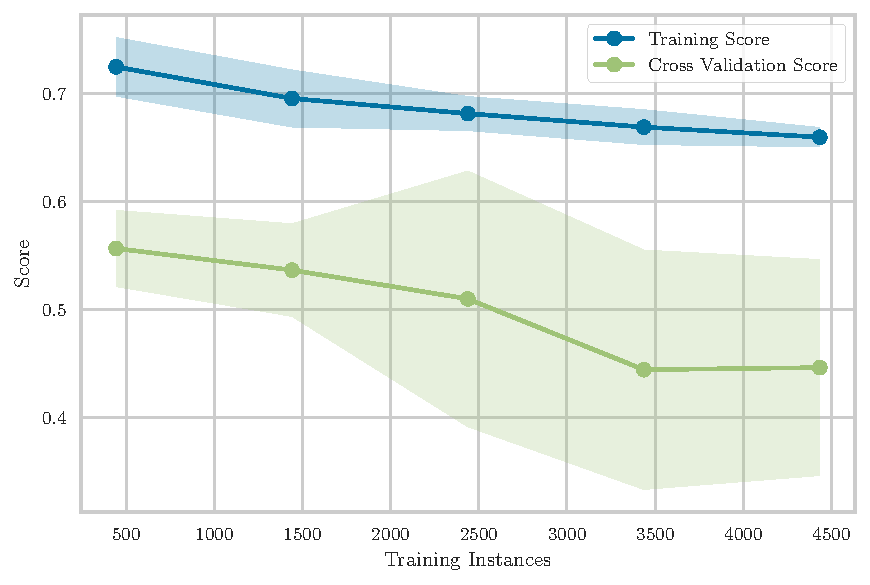
\includegraphics[width=\textwidth]{images/learning_curve.pdf}
    \end{center}
    \caption{Learning Curves for XGBoost Classifier Showing Training and Cross-Validation Performance Across Dataset Sizes}
    \label{fig:learning_curve}
\end{figure}

The learning curve demonstrates fundamental aspects of the model's predictive capacity and its ability to generalize to unseen data. The training score, representing the model's performance on the data used for parameter estimation, begins at approximately 87\% accuracy for smaller datasets and stabilizes around 70\% as the training set expands to include the full historical sample of over 4,500 observations. The cross-validation score, which measures the model's performance on held-out data not used during training, provides a more conservative and realistic assessment of predictive capability (Harrison, 2023). This cross-validation approach involves systematically withholding portions of the data during training and evaluating performance on these unseen observations, thereby providing an unbiased estimate of how the model will perform on future, unknown bond issuances.

The cross-validation score exhibits a trajectory starting near 53\% and converging toward 43\% for larger training sets. This performance pattern reveals several critical aspects of the model's behavior. The approximately 25 basis point gap between training and validation performance indicates the presence of some overfitting, which is expected given the complexity of financial relationships and the relatively modest dataset size. However, the convergence of both curves at larger sample sizes demonstrates that the model successfully captures systematic patterns in the data rather than merely memorizing noise. The cross-validation performance of 43\% represents a meaningful improvement over random classification (33\% for the ternary framework), confirming the model's ability to extract predictive signal from the identified features.

The stabilization of both learning curves suggests that additional training data would yield diminishing returns in terms of improved predictive accuracy. This plateau indicates that the model has successfully identified the maximum extractable signal from the current feature set and that further performance improvements would likely require either additional predictive variables or alternative modeling approaches.

\section{Classification Results and Investment Outcomes}

The model's practical utility emerges through its classification performance and resulting investment outcomes. The confusion matrix presented in Figure \ref{fig:confusion_matrix} illustrates the model's classification decisions across 1,776 bond evaluations during the backtest period.

\begin{figure}[h]
    \begin{center}
        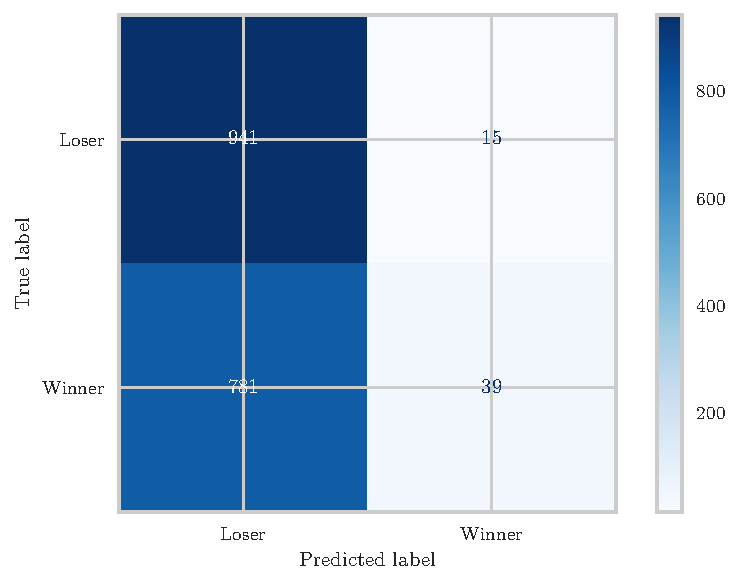
\includegraphics[width=\textwidth]{images/confusion_matrix.pdf}
    \end{center}
    \caption{Confusion Matrix for Overall Backtest Period Showing Predicted Versus Actual Bond Classifications}
    \label{fig:confusion_matrix}
\end{figure}

The confusion matrix reveals the model's highly conservative approach to winner identification, consistent with the optimization objective that prioritizes precision over recall. Of the bonds evaluated, the model classified 1,700 as likely underperformers and only 76 as potential outperformers. This extreme selectivity reflects both the challenge of identifying genuine new issue premium opportunities in the investment-grade market and the deliberate optimization toward the highest-conviction selections.

The precision metrics provide particularly relevant insights for practical implementation. The model achieves 72\% precision in identifying winners, meaning that approximately seven out of ten bonds predicted to outperform actually do so. This level of accuracy represents substantial value for portfolio managers, as it significantly exceeds the market's natural success rate. The model demonstrates 55\% precision in identifying losers, with a weighted average precision of 63\% across both classifications.

The recall patterns highlight the model's extremely selective criteria, achieving 98\% recall for losers but only 7\% recall for winners. This highly asymmetric performance reflects the optimization framework's emphasis on minimizing false positives in winner selection, as incorrectly selected bonds impose direct costs on portfolio performance. The low recall for winners represents a deliberate trade-off inherent in the threshold optimization process rather than a fundamental limitation of the model's predictive capability.

Table \ref{tab:backtest_performance} summarizes the key investment performance metrics over the full evaluation period, demonstrating the economic value generated by the model's selective approach.

\begin{table}[htbp]
\centering
\caption{Investment Performance Metrics for New Issue Premium Strategy}
\label{tab:backtest_performance}
\begin{tabular}{lc}
\hline
\textbf{Performance Metric} & \textbf{Full Period} \\
\hline
Average Active Return (RA) & 36 bp \\
Average Market Participation (MP) & 4.5\% \\
Optimization Objective (MP $\times$ RA) & 1.6 \\
Average Selected Bond Return & 21 bp \\
\hline
\end{tabular}
\end{table}

The active return of 36 basis points represents the core measure of the model's economic value, quantifying the average outperformance of the model-selected portfolio relative to an equal-weighted benchmark comprising all new issuances during the evaluation period. Given the five-day investment horizon, this 36 basis point premium represents substantial value that compounds significantly over multiple investment cycles. The market participation rate of 4.5\% demonstrates the model's highly selective approach, participating in fewer than one out of every twenty new issuances while concentrating investments in the highest-conviction opportunities.

The temporal performance analysis, illustrated in Figure \ref{fig:monthly_performance}, reveals the consistency of the model's outperformance across different market environments. The strategy demonstrates sustained outperformance across most months, with particularly strong results during periods of market stress, notably achieving nearly 100 basis points of return during November 2024 compared to negative market averages.

\begin{figure}[h]
    \begin{center}
        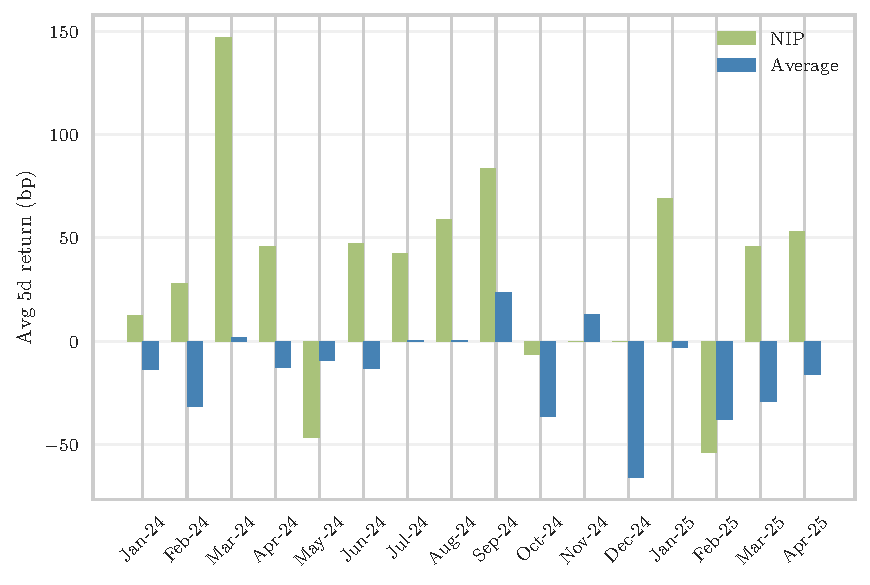
\includegraphics[width=\textwidth]{images/monthly_comparison.pdf}
    \end{center}
    \caption{Monthly Performance Comparison: New Issue Premium Strategy Versus Market Average Returns (January 2024 - April 2025) Note. Returns measured in basis points (bp).}
    \label{fig:monthly_performance}
\end{figure}

This temporal consistency supports the robustness of the underlying feature relationships, suggesting that the model captures systematic patterns in new issue pricing that persist across varying market cycles rather than relying on specific market conditions or temporary anomalies. The optimization objective of 1.6, calculated as the product of market participation and active return, provides a composite measure of the strategy's risk-adjusted performance, representing a meaningful improvement over passive participation in the new issue market.

\section{Risk-Adjusted Performance Analysis}

The model's investment strategy demonstrates strong risk-adjusted characteristics that enhance its practical utility for institutional implementation. Table \ref{tab:risk_metrics} presents comprehensive risk and performance statistics over the evaluation period.

\begin{table}[htbp]
\centering
\caption{Risk-Adjusted Performance Statistics for Investment Strategy}
\label{tab:risk_metrics}
\begin{tabular}{lc}
\hline
\textbf{Risk Metric} & \textbf{Value} \\
\hline
Average Monthly Return & 36 bp \\
Return Volatility & 44 bp \\
Sharpe-like Ratio & 0.81 \\
Maximum Drawdown & -47 bp \\
Win Rate & 75\% \\
Best Monthly Performance & 147 bp \\
Worst Monthly Performance & -47 bp \\
Market Outperformance Rate & 81\% \\
\hline
\end{tabular}
\end{table}

The strategy's Sharpe-like ratio of 0.81 indicates strong risk-adjusted returns, demonstrating that the 36 basis point average monthly active return is achieved with reasonable volatility of 44 basis points. This risk-return profile compares favorably to many traditional fixed-income strategies, particularly considering the concentrated nature of the portfolio selections. The 75\% win rate, with positive performance in 12 out of 16 months, provides evidence of consistent value generation rather than dependence on occasional large gains.

The maximum drawdown of 47 basis points, occurring during the worst-performing month, represents a moderate downside risk that aligns with the strategy's conservative selection criteria. The asymmetric return distribution, with average positive monthly returns of 54 basis points compared to average negative returns of 18 basis points, demonstrates the model's ability to capture significant upside while limiting downside exposure. The 81\% market outperformance rate confirms that the strategy generates positive active returns in the vast majority of evaluation periods.

\section{Practical Implementation and Strategic Considerations}

The model's extremely conservative winner identification approach provides multiple layers of risk management that enhance its practical utility for institutional investors. The 72\% precision in winner selection minimizes false positive classifications, reducing the likelihood of investing in bonds that may underperform due to unidentified risk factors. The 4.5\% market participation rate significantly concentrates investments in the highest-conviction opportunities while maintaining sufficient selectivity for institutional quality requirements.

The 36 basis point active return, when considered within the context of typical institutional new issue investment frequencies, represents substantial value creation potential. For portfolio managers regularly participating in the primary bond market, this level of outperformance contributes meaningfully to overall portfolio returns while preserving capital efficiency through highly selective deployment. The systematic, data-driven approach provides a quantitative framework that complements traditional qualitative analysis methods, enabling portfolio managers to process multiple risk factors simultaneously and weight them according to their predictive importance.

The combination of strong risk-adjusted returns (Sharpe-like ratio of 0.81) and high market outperformance rate (81\%) supports integration into existing fixed-income investment processes as a specialized alpha-generation tool. However, successful implementation requires recognition that the model serves as a systematic enhancement to traditional analysis rather than a standalone investment solution. The extremely concentrated selection approach (4.5\% participation) necessitates integration within broader portfolio strategies to maintain adequate diversification and capital deployment efficiency.

\section{Model Limitations and Optimization Trade-offs}

The model's performance characteristics reflect deliberate optimization choices rather than fundamental limitations in predictive capability. The 7\% recall rate for winners, while appearing very low in isolation, results from the threshold parameter $w$ optimization process that maximizes the investment objective function $MP \times RA$. The model possesses the capability to identify a significantly higher proportion of actual winners by adjusting this threshold toward greater inclusivity, but such adjustments would necessarily reduce precision and overall economic value. The current configuration represents the optimal balance between market participation and active return, deliberately sacrificing recall to maximize the practical utility of the investment strategy.

The 43\% cross-validation accuracy, though superior to random classification, reflects the inherent difficulty of predicting short-term bond price movements in liquid, efficiently-traded markets rather than inadequacies in the modeling approach. This performance level demonstrates that systematic patterns exist in new issue pricing, even within the constraints of market efficiency, and that quantitative methods can successfully extract economic value from these patterns.

The temporal concentration of the backtest period provides recent and relevant market conditions but limits assessment of model performance across different credit cycles and interest rate environments. Extended evaluation periods incorporating various market regimes would enhance confidence in the model's robustness, though the consistent performance across the available evaluation period suggests reasonable stability in the underlying relationships.

The model's reliance on historical feature relationships assumes persistence of identified patterns in future market conditions. While changes in market structure, investor behavior, or regulatory environment could potentially impact effectiveness, the economic intuition underlying the selected features and the demonstrated consistency of outperformance provide reasonable confidence in the model's continued utility for enhancing new issue investment decisions in the European investment-grade corporate bond market.
\chapter{Conclusion}
\label{ch:conclusion}

\section{Summary of Findings}

This research demonstrates that machine learning algorithms can effectively predict short-term outperformance of European investment grade corporate bonds using variables available at issuance. The XGBoost classifier achieved 72\% precision in identifying outperforming bonds while maintaining a conservative market participation rate of 4.5\%. These results indicate that systematic patterns exist in the pricing of new issues that can be exploited through quantitative methods, even within relatively efficient markets. When implemented as an investment strategy during the evaluation period from January 2024 through April 2025, the model generated an average active return of 36 basis points over five-day investment horizons with a Sharpe-like ratio of 0.81 and a 75\% win rate.

The results confirm the economic importance of several features in predicting new-issue premium opportunities. First-time issuers demonstrated significantly higher excess returns compared to seasoned issuers, supporting the existence of an information asymmetry premium. The Z-spread metrics, the maturity of the bonds, and macroeconomic factors such as inflation and the direction of the market also showed strong predictive power. The model's success in translating these complex, multidimensional relationships into actionable investment signals demonstrates the viability of machine learning approaches for enhancing traditional fixed-income selection methodologies.

\section{Limitations and Future Research}

The performance characteristics of the model reflect deliberate optimization choices rather than fundamental limitations in predictive capability. The 7\% recall rate for winners, while very low in isolation, is the result of the threshold parameter optimization process that maximizes the investment objective function $MP \times RA$. The model possesses the capability to identify a significantly higher proportion of actual winners by adjusting this threshold toward greater inclusivity, but such adjustments would necessarily reduce precision and overall economic value.

The 43\% cross-validation accuracy, though superior to random classification, reflects the inherent difficulty of predicting short-term bond price movements in liquid, efficiently traded markets. This performance level demonstrates that while systematic patterns exist in new-issue pricing, substantial unpredictability remains that cannot be captured through currently available features. Although market sentiment indicators were incorporated into the present analysis, future research could benefit from access to order book dynamics during the issuance process, which were not accessible through the Refinitiv database utilized in this study. Such data could potentially provide valuable insights into demand patterns and pricing pressure that are not captured by currently available features.

Although the current evaluation period (16 months) provides valuable insight into the model's performance, extending the backtest horizon would offer additional validation across different market environments. However, such extensions face practical challenges due to the temporal distribution bias in available bond data, with significantly more observations concentrated in recent years, as shown in Figure 3.1. This characteristic of the data makes historically extensive backtests challenging with conventional data sources. Future research could leverage specialized financial data platforms such as Bloomberg to access more complete historical bond records, potentially enabling a comprehensive performance assessment across multiple credit cycles and interest rate environments. Despite these constraints, the consistent performance observed in varying monthly conditions within the evaluation period suggests promising robustness.

The model's reliance on historical feature relationships assumes persistence of identified patterns in future market conditions. While changes in market structure, investor behavior, or regulatory environment could potentially impact effectiveness, the economic intuition underlying the selected features provides reasonable confidence in their continued relevance. However, future research should investigate the stability of these relationships over extended periods of time and across different market environments.

\section{Addressing Potential Concerns}

Critics may question whether the observed outperformance reflects genuine alpha generation or simply compensation for unidentified risk factors not captured in the model. The relatively modest dataset size (7,320 bonds) could suggest limitations in the model's ability to fully differentiate signal from noise in bond performance data.

Moreover, skeptics might argue that market efficiency should eventually eliminate exploitable patterns as they become widely recognized. If the new-issue premium represents a persistent anomaly, its continued existence seems to contradict efficient market assumptions, raising questions about its sustainability as an investment strategy.

From a practical implementation perspective, the model's focus on a short-term investment horizon (five days) could potentially conflict with syndicate banks' preferences for allocating new issues to investors with longer-term holding intentions. Syndicate desks may gradually favor buyers who demonstrate commitment to holding positions beyond the immediate post-issuance period. However, even if such allocation challenges emerge, the model's predictive capabilities remain valuable: the identified bonds could simply be held for longer periods, albeit with potentially different return profiles than those observed in the five-day window.

On the other hand, the new issue premium likely persists precisely because of structural market factors that resist arbitrage. The inherent information asymmetry between issuers and investors, combined with liquidity considerations and investor behavior patterns, creates persistent pricing inefficiencies that cannot be easily eliminated. The model's strong risk-adjusted performance metrics and high win rate suggest that the identified patterns reflect genuine structural market characteristics rather than statistical artifacts.

Furthermore, the highly selective approach of the model (4. 5\% market participation) creates natural barriers to the limitations of the capacity of the strategy. Even if widely adopted, the approach would impact only a small fraction of the market, allowing the premium to persist. The model effectively serves as a systematic enhancement to traditional analysis rather than a replacement, complementing existing investment processes with quantitative insights that human analysts might overlook.

In conclusion, this research demonstrates that machine learning can meaningfully enhance investment decision making in European investment-grade corporate bond markets. By systematically identifying high-precision new-issue premium opportunities, the approach offers portfolio managers a valuable tool for alpha generation while maintaining appropriate risk controls. Although limitations exist, the results establish a compelling foundation for integrating quantitative methods into fixed-income investment processes, potentially transforming how portfolio managers approach the evaluation and selection of new issues.

% ------------------
% |    Appendix    |
% ------------------
\appendix
\pagenumbering{Roman}
\setcounter{page}{1}
\chapter{Appendix}

\section{Spearman Correlation Heatmap}
\addcontentsline{toc}{section}{Spearman Correlation Heatmap}

\begin{center}
\begin{minipage}{\textwidth}
    \centering
    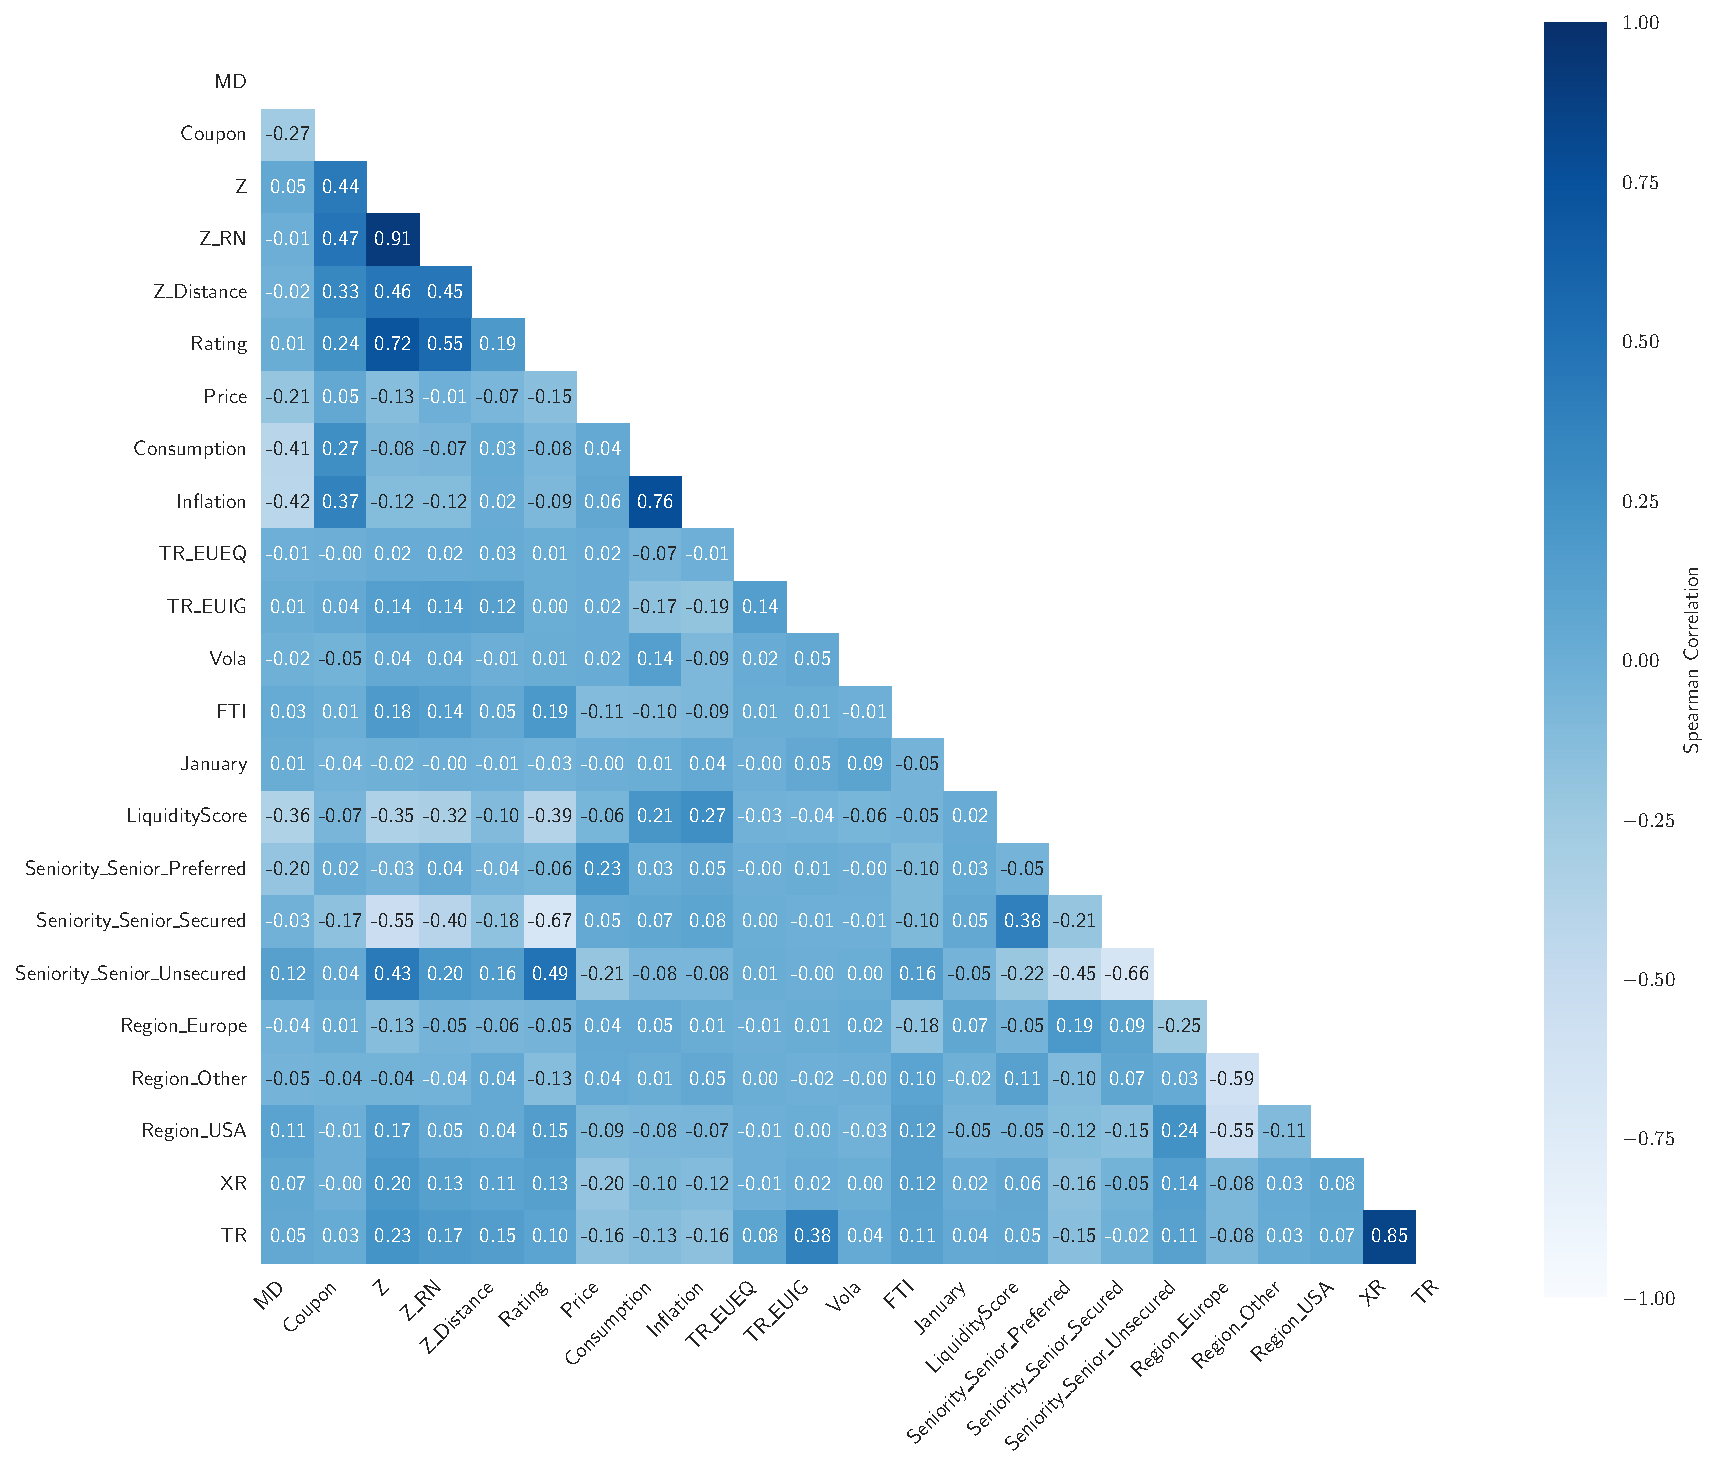
\includegraphics[width=\textwidth]{images/correlation_heatmap.pdf}
    \captionof{figure}{Spearman Correlation Matrix for Model Features and Dependent Variables}
    \label{fig:correlation_heatmap}
\end{minipage}
\end{center}

\section{Feature t-statistics Heatmap}
\addcontentsline{toc}{section}{Feature t-statistics Heatmap}

\vspace{1em}

\begin{center}
\begin{minipage}{\textwidth}
    \centering
    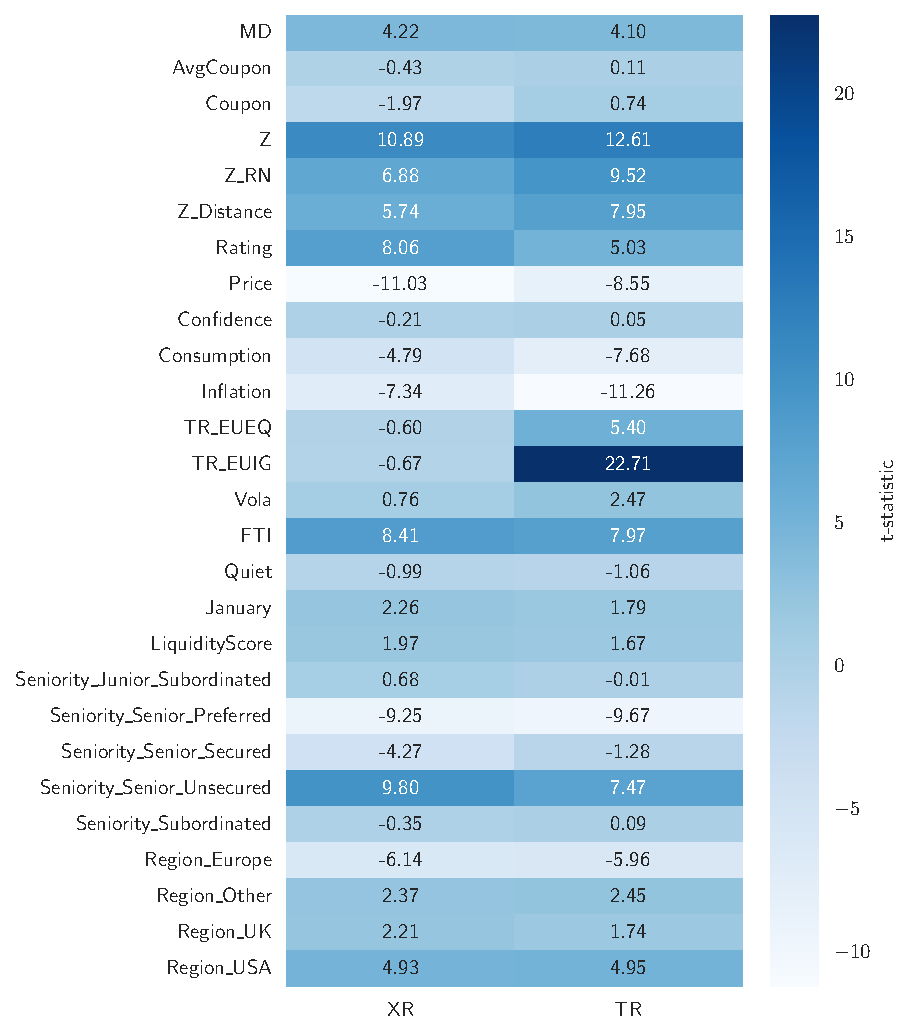
\includegraphics[width=\textwidth]{images/feature_t_statistics.pdf}
    \captionof{figure}{Feature Importance T-Statistics Heatmap for Excess Return (XR) and Total Return (TR) Models}
    \label{fig:feature_tstat}
\end{minipage}
\end{center}


\section{Feature t-statistics Table}
\addcontentsline{toc}{section}{Feature t-statistics Heatmap Table}

\begin{center}
\begin{minipage}{\textwidth}
    \centering
    \small
    \begin{tabular}{lcccccc}
    \toprule
    \textbf{Feature} & \textbf{t\_XR} & \textbf{p\_XR} & \textbf{Sig\_XR} & \textbf{t\_TR} & \textbf{p\_TR} & \textbf{Sig\_TR} \\
    \midrule
    MD & 4.2249 & <0.0001 & *** & 4.0987 & <0.0001 & *** \\
    AvgCoupon & -0.4263 & 0.6699 &  & 0.1096 & 0.9127 &  \\
    Coupon & -1.9663 & 0.0493 & ** & 0.7352 & 0.4622 &  \\
    Z & 10.8945 & <0.0001 & *** & 12.6075 & <0.0001 & *** \\
    Z\_RN & 6.8803 & <0.0001 & *** & 9.5164 & <0.0001 & *** \\
    Z\_Distance & 5.7363 & <0.0001 & *** & 7.9503 & <0.0001 & *** \\
    Rating & 8.0607 & <0.0001 & *** & 5.0331 & <0.0001 & *** \\
    Price & -11.0253 & <0.0001 & *** & -8.5452 & <0.0001 & *** \\
    Confidence & -0.2129 & 0.8314 &  & 0.0523 & 0.9583 &  \\
    Consumption & -4.7937 & <0.0001 & *** & -7.6849 & <0.0001 & *** \\
    Inflation & -7.3394 & <0.0001 & *** & -11.2597 & <0.0001 & *** \\
    TR\_EUEQ & -0.5987 & 0.5494 &  & 5.4030 & <0.0001 & *** \\
    TR\_EUIG & -0.6750 & 0.4997 &  & 22.7080 & <0.0001 & *** \\
    Vola & 0.7550 & 0.4503 &  & 2.4747 & 0.0134 & ** \\
    FTI & 8.4112 & <0.0001 & *** & 7.9678 & <0.0001 & *** \\
    Quiet & -0.9908 & 0.3218 &  & -1.0583 & 0.2899 &  \\
    January & 2.2591 & 0.0239 & ** & 1.7878 & 0.0739 & * \\
    LiquidityScore & 1.9743 & 0.0484 & ** & 1.6710 & 0.0948 & * \\
    Seniority\_Junior\_Subordinated & 0.6799 & 0.4966 &  & -0.0060 & 0.9952 &  \\
    Seniority\_Senior\_Preferred & -9.2537 & <0.0001 & *** & -9.6705 & <0.0001 & *** \\
    Seniority\_Senior\_Secured & -4.2747 & <0.0001 & *** & -1.2762 & 0.2019 &  \\
    Seniority\_Senior\_Unsecured & 9.8046 & <0.0001 & *** & 7.4691 & <0.0001 & *** \\
    Seniority\_Subordinated & -0.3460 & 0.7294 &  & 0.0862 & 0.9313 &  \\
    Region\_Europe & -6.1352 & <0.0001 & *** & -5.9560 & <0.0001 & *** \\
    Region\_Other & 2.3687 & 0.0179 & ** & 2.4531 & 0.0142 & ** \\
    Region\_UK & 2.2089 & 0.0272 & ** & 1.7426 & 0.0815 & * \\
    Region\_USA & 4.9261 & <0.0001 & *** & 4.9462 & <0.0001 & *** \\
    \bottomrule
    \end{tabular}
    \captionof{table}{Statistical Significance Tests for Model Features Across Excess Return and Total Return Datasets Note.}
    \caption*{\textit{Significance:} * $p<0.10$, ** $p<0.05$, *** $p<0.01$}
    \label{tab:feature_t_statistics}
\end{minipage}
\end{center}

\section{Feature Importance Plot}
\addcontentsline{toc}{section}{Feature Importance Plot}

\begin{center}
\begin{minipage}{\textwidth}
    \centering
    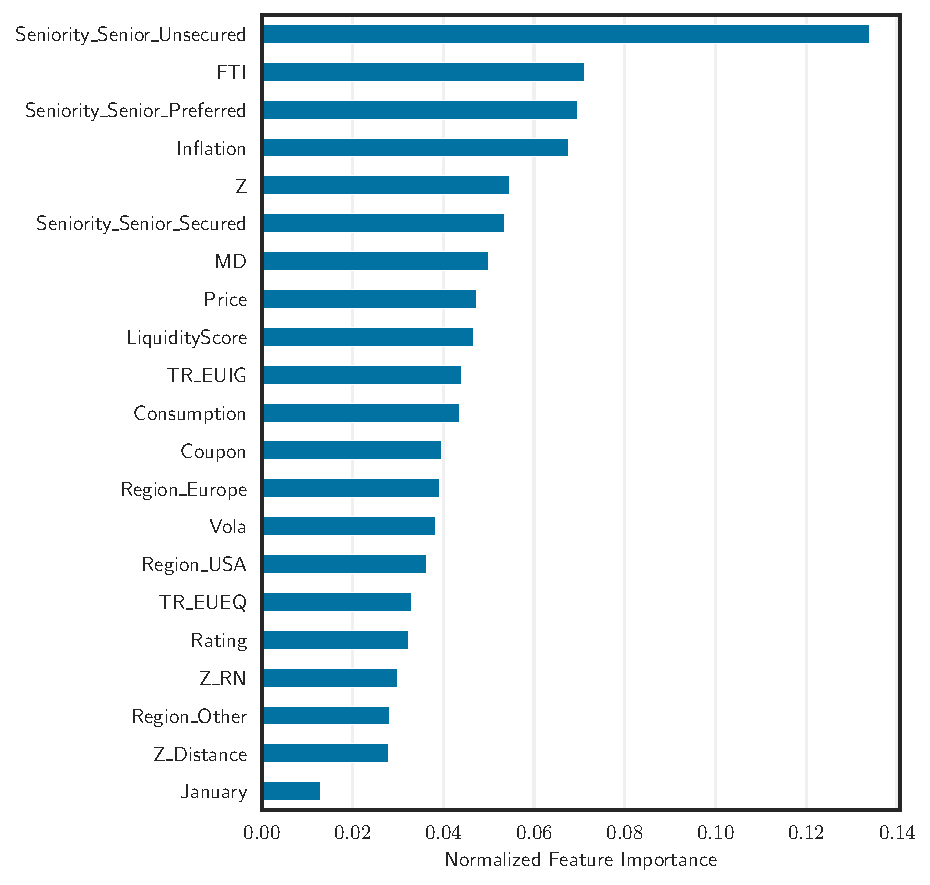
\includegraphics[width=\textwidth]{images/feature_importance.pdf}
    \captionof{figure}{Normalized Feature Importance Rankings from XGBoost Classifier}
    \label{fig:feature_importance}
\end{minipage}
\end{center}

% ----------------------
% |    Bibliography    |
% ----------------------
\printbibliography[title=References]

% ----------------------
% |    Declarations    |
% ----------------------
\chapter*{AI Declaration}
\thispagestyle{empty}

This bachelor thesis was completed with the assistance of several artificial intelligence tools that supported different aspects of the research and writing process. The primary tools employed were ChatGPT in two versions (o3 for conceptual explanations and idea generation, o4-mini-high for coding assistance), Claude AI (Sonnet 3.7) and Quilbot for language enhancement, and Elicit and Perplexity (Pro) for academic source identification.

These tools served distinct functions throughout the thesis development. ChatGPT o3 helped clarify complex theoretical concepts and generate initial ideas during the early research phases. The o4-mini-high variant proved helpful for debugging code. Claude AI and Quilbot enhanced the clarity and academic tone of written content. Elicit and Perplexity Pro accelerated the literature review process by identifying relevant academic papers and sources more efficiently than traditional database searches alone.

The integration of these AI tools significantly enhanced productivity across multiple dimensions of the research process. Coding efficiency improved substantially through automated error identification and debugging assistance, reducing the time required for technical implementation. Source identification became considerably faster, particularly for discovering interdisciplinary connections and recent publications that might have been overlooked through conventional search methods.

However, the experience also revealed important limitations that required careful oversight. AI tools occasionally suggested irrelevant sources that needed independent verification before incorporation into the research. More significantly, the tools demonstrated limited utility for highly specialized tasks, particularly data extraction procedures requiring specific API implementations. These technical limitations became apparent when addressing novel methodological requirements that fell outside the scope of the AI systems' training data.
\chapter*{Affidavit}
\thispagestyle{empty}

I hereby declare that I have written this thesis on my own and with no other help than the literature and other supportive material listed in the appendix. Citations of sentences and parts of sentences are declared as such, while other imitations are clearly marked and linked to original sources with regard to the extent and intention of the statements made. This thesis has never been handed in to any examination authority before and it is also not yet published.

\vspace{1cm}

\noindent
Vallendar, May 23, 2025

\vspace{1cm}

\noindent
Lukas Jonathan Michael

\vspace{1cm}

\noindent
\begin{minipage}{0.45\textwidth}
\centering
Place, Date \\[1.5cm]
\rule{4cm}{0.4pt}
\end{minipage}
\hfill
\begin{minipage}{0.45\textwidth}
\centering
Signature \\[1.5cm]
\rule{4cm}{0.4pt}
\end{minipage}

\end{document}